%!TEX program = xelatex

\documentclass[UTF8]{ctexart}
\usepackage{ctex}

\CTEXsetup[format={\Large\bfseries}]{section}

\usepackage[version=3]{mhchem} % Package for chemical equation typesetting
\usepackage{siunitx} % Provides the \SI{}{} and \si{} command for typesetting SI units
\usepackage{graphicx} % Required for the inclusion of images
\graphicspath{{assets/}}
\usepackage{natbib} % Required to change bibliography style to APA
\usepackage{amsmath} % Required for some math elements 
\usepackage{amssymb}
\usepackage[hidelinks]{hyperref}
\usepackage{makecell} % 3 Packages for flexible tabular
\usepackage{multirow}
\usepackage{multicol}

\usepackage{pdfpages}  % include pdf pages for original data etc.

\usepackage{geometry}% 版面大小
\geometry{a4paper,scale=0.7}

\usepackage{fontspec}

\setCJKfamilyfont{hwxk}{STXingkai}% 字体
\newcommand{\hwxk}{\CJKfamily{hwxk}}

\usepackage{fancyhdr}% 页眉页脚
\fancypagestyle{EE_Digital1Exp_template}{
    \fancyhead[L]{\Large {\hwxk 南京大学电子科学与工程学院}}
    \fancyhead[R]{数字系统1实验报告}
    \fancyfoot[c]{- \thepage \ -}
    \renewcommand\footrulewidth{0pt}
}

% 4级目录
\setcounter{secnumdepth}{4}
\setcounter{tocdepth}{4}

\usepackage{graphicx} % Packages for figures
\usepackage{caption2}
\usepackage{subfigure}
\usepackage{float}


%设置图片、表格编号
\renewcommand{\thetable}{\thesubsection{}-\arabic{table}}
\renewcommand{\thefigure}{\thesubsection{}-\arabic{figure}}
\renewcommand{\thefigure}{\thesubsection{}-\arabic{equation}}
\usepackage{amsmath}
\numberwithin{figure}{subsection}
\numberwithin{table}{subsection}
\numberwithin{equation}{subsection}

\setlength\parindent{6pt} % Removes all indentation from paragraphs

\renewcommand{\labelenumi}{\alph{enumi}.} % Make numbering in the enumerate environment by letter rather than number (e.g. section 6)

%\usepackage{times} % Uncomment to use the Times New Roman font

%----------------------------------------------------------------------------------------
%	DOCUMENT INFORMATION
%----------------------------------------------------------------------------------------

\title{\textbf{实验2\ 计数器}} % Title

\author{电子科学与工程学院 刘时宜 201180078} % Author name

\date{} % Date for the report

\begin{document}

\pagestyle{EE_Digital1Exp_template}

\maketitle % Insert the title, author and date

\begin{center}
    \begin{tabular}{l r}
    实验日期: & 2021年11月23日 \\ % Date the experiment was performed
    指导老师: & 高健 % Instructor/supervisor
    \end{tabular}
    \par 点击目录、书签栏、以及行文中的图表标号的均可跳转至相应页面
    \end{center}
    
% If you wish to include an abstract, uncomment the lines below
% \begin{abstract}
% Abstract text
% \end{abstract}

\tableofcontents

\section{实验目的}
\begin{enumerate}
    \item 验证计数器工作原理
    \item 利用已有计数器模块设计实现其他进制的计数器模块
    \item 利用计数器设计实现秒表
\end{enumerate}

\section{实验仪器与主要器材}
\begin{center}
    \begin{tabular}{ll}
        \textbf{仪器:} & \\
        Basys3 FPGA 开发板 & 1台\\
        KEYSIGHT DSOX1102AG 示波器 & 1台\\
        示波器高频探头 & 1套\\
        ROGOL DM3068 万用表 & 1台\\
        \textbf{软件:} & \\
        Multisim & 14.1 \\
        Digilent Adept & 2.19.2 \\
        Vivado & 2015.4 \\
        \textbf{耗材:} & \\
        导线 & 若干 \\
    \end{tabular}
\end{center}

\section{实验原理}
\par 计数器在数字系统中广泛使用,可以用于对时钟脉冲计数、分频、定时、进行数学运算等。
\par 计数器种类繁多。如果按照计数器中的触发器是否同时翻转分类,可以将计数器分为同步式和异步式两种。同步计数器中,当时钟脉冲输入时触发器的翻转同时发生,而在异步计数器中,触发器的翻转又先后,不是同时发生的。
\par 如果按照计数过程中数字的增减分类,可以分为加法计数器、减法计数器以及可逆计数器。随着计数脉冲的不断输入而作递增的计数器称为加法计数器,作递减计数的称为减法计数器,可增可减的称为可逆计数器。
\par 本实验中用到的计数器多为异步加法计数器。

\section{实验过程}
\subsection{十进制加法计数器}
开发板连接至电脑后下载已经编译好的十进制计数器bit流文件。
\par 将\(SW_0\)、\(SW_1\)开关均拨至断开位置,观察计数器数字缓慢变化。将\(SW_1\)闭合,使用示波器观察计数器各输出引脚波形。
\subsubsection{实验结果}
\(SW_0 = SW_1 = 0\)时,时钟周期为\SI{0.75}{\Hz},计数器数字缓慢变化。观察到十进制计数器共有10个稳态,分别显示数字\(0\sim 9\),如图\ref{10counter_slow}所示。

\begin{figure}[H]
    \centering
    \subfigure[0]{
    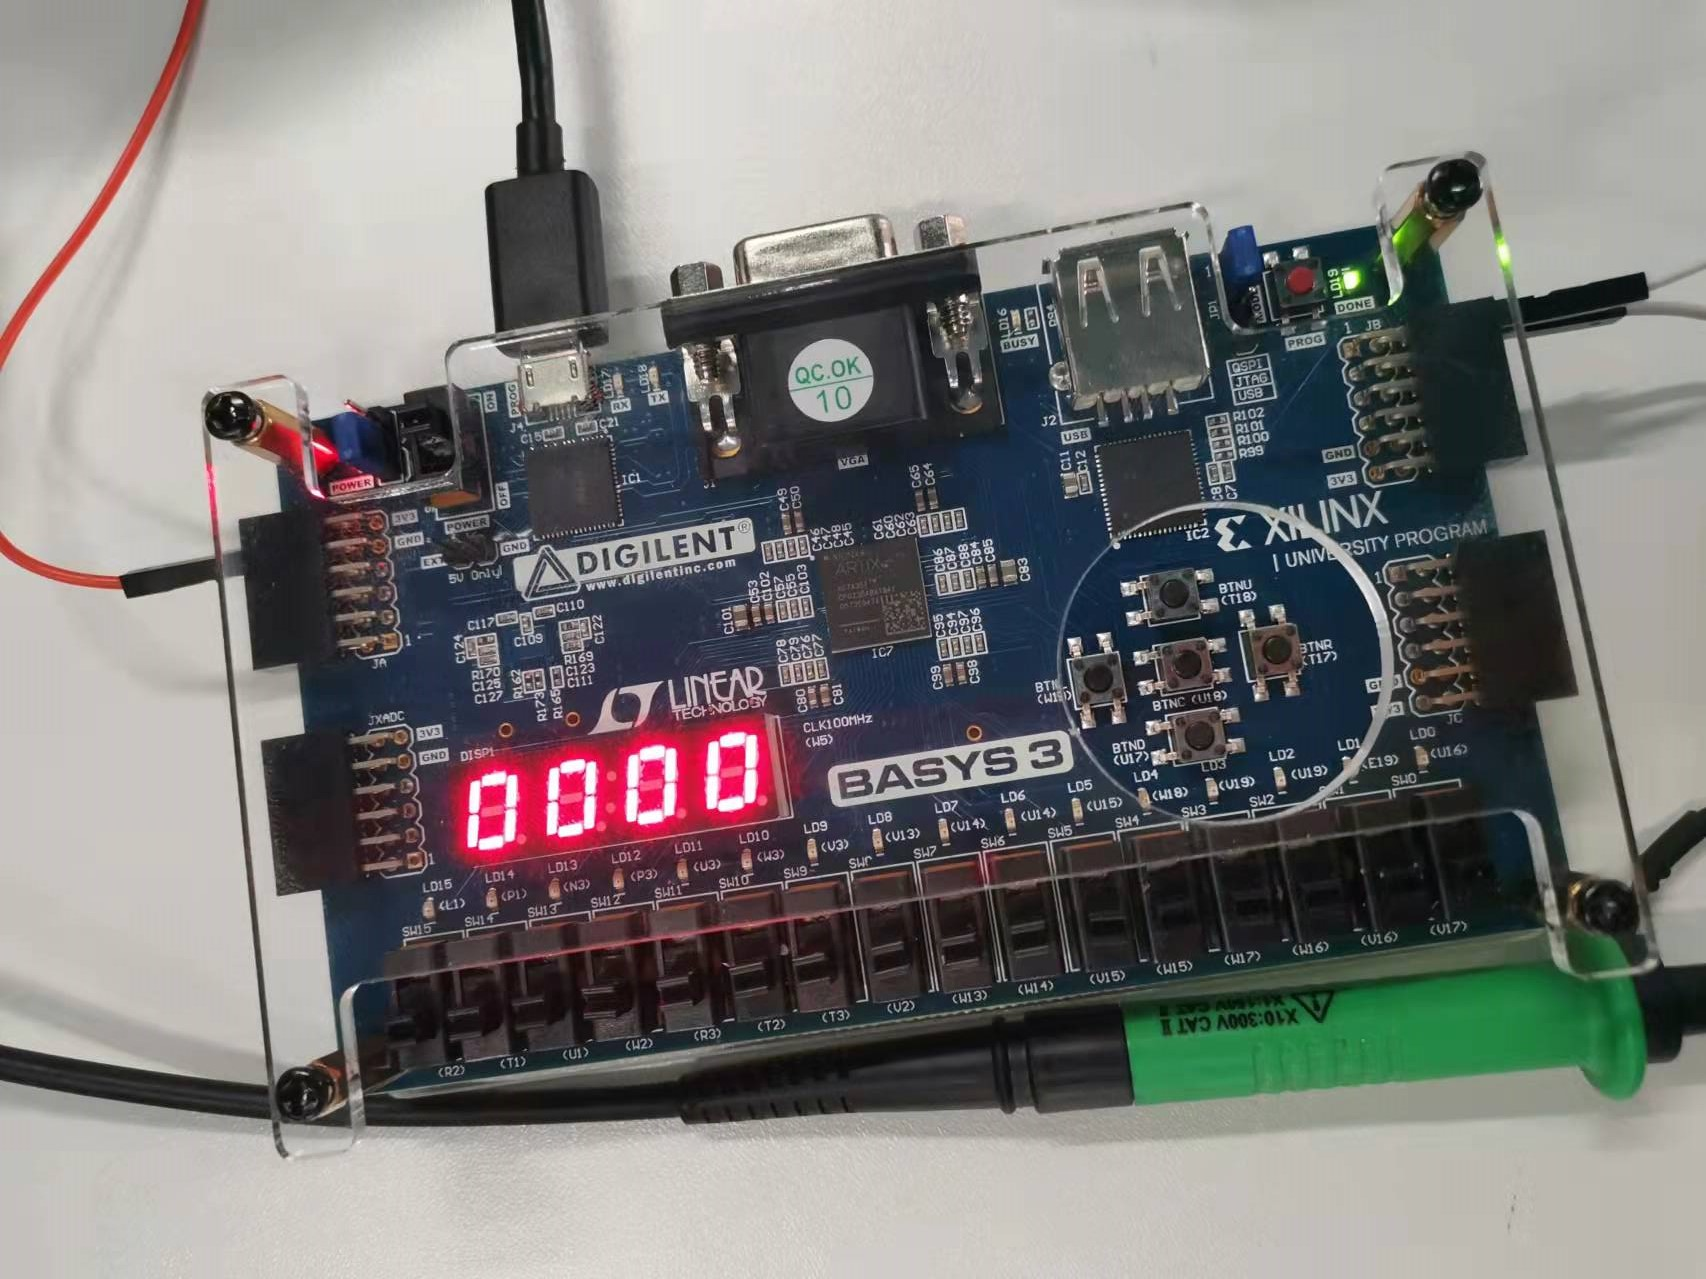
\includegraphics[width=0.3\textwidth]{original pic/0.jpg}}
    \subfigure[1]{
    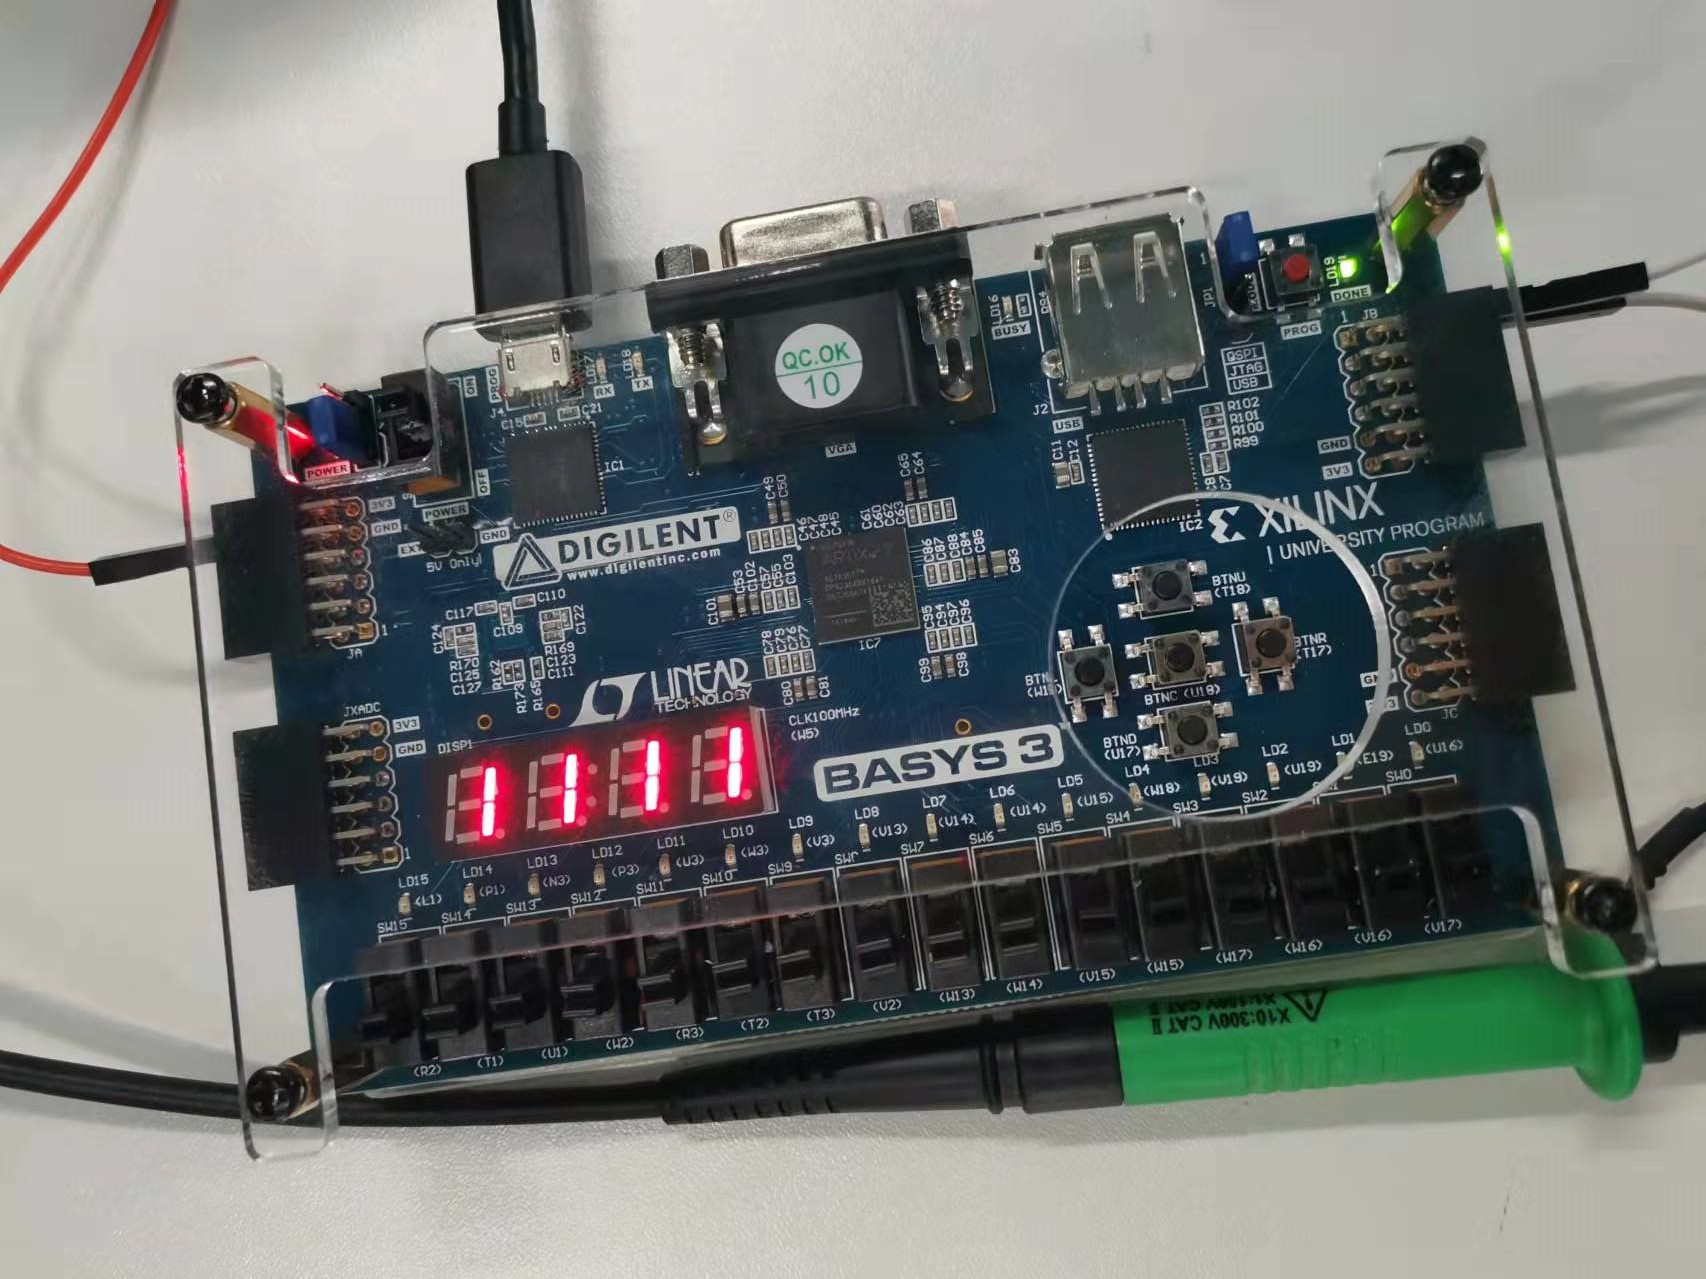
\includegraphics[width=0.3\textwidth]{original pic/1.jpg}}
    \subfigure[2]{
    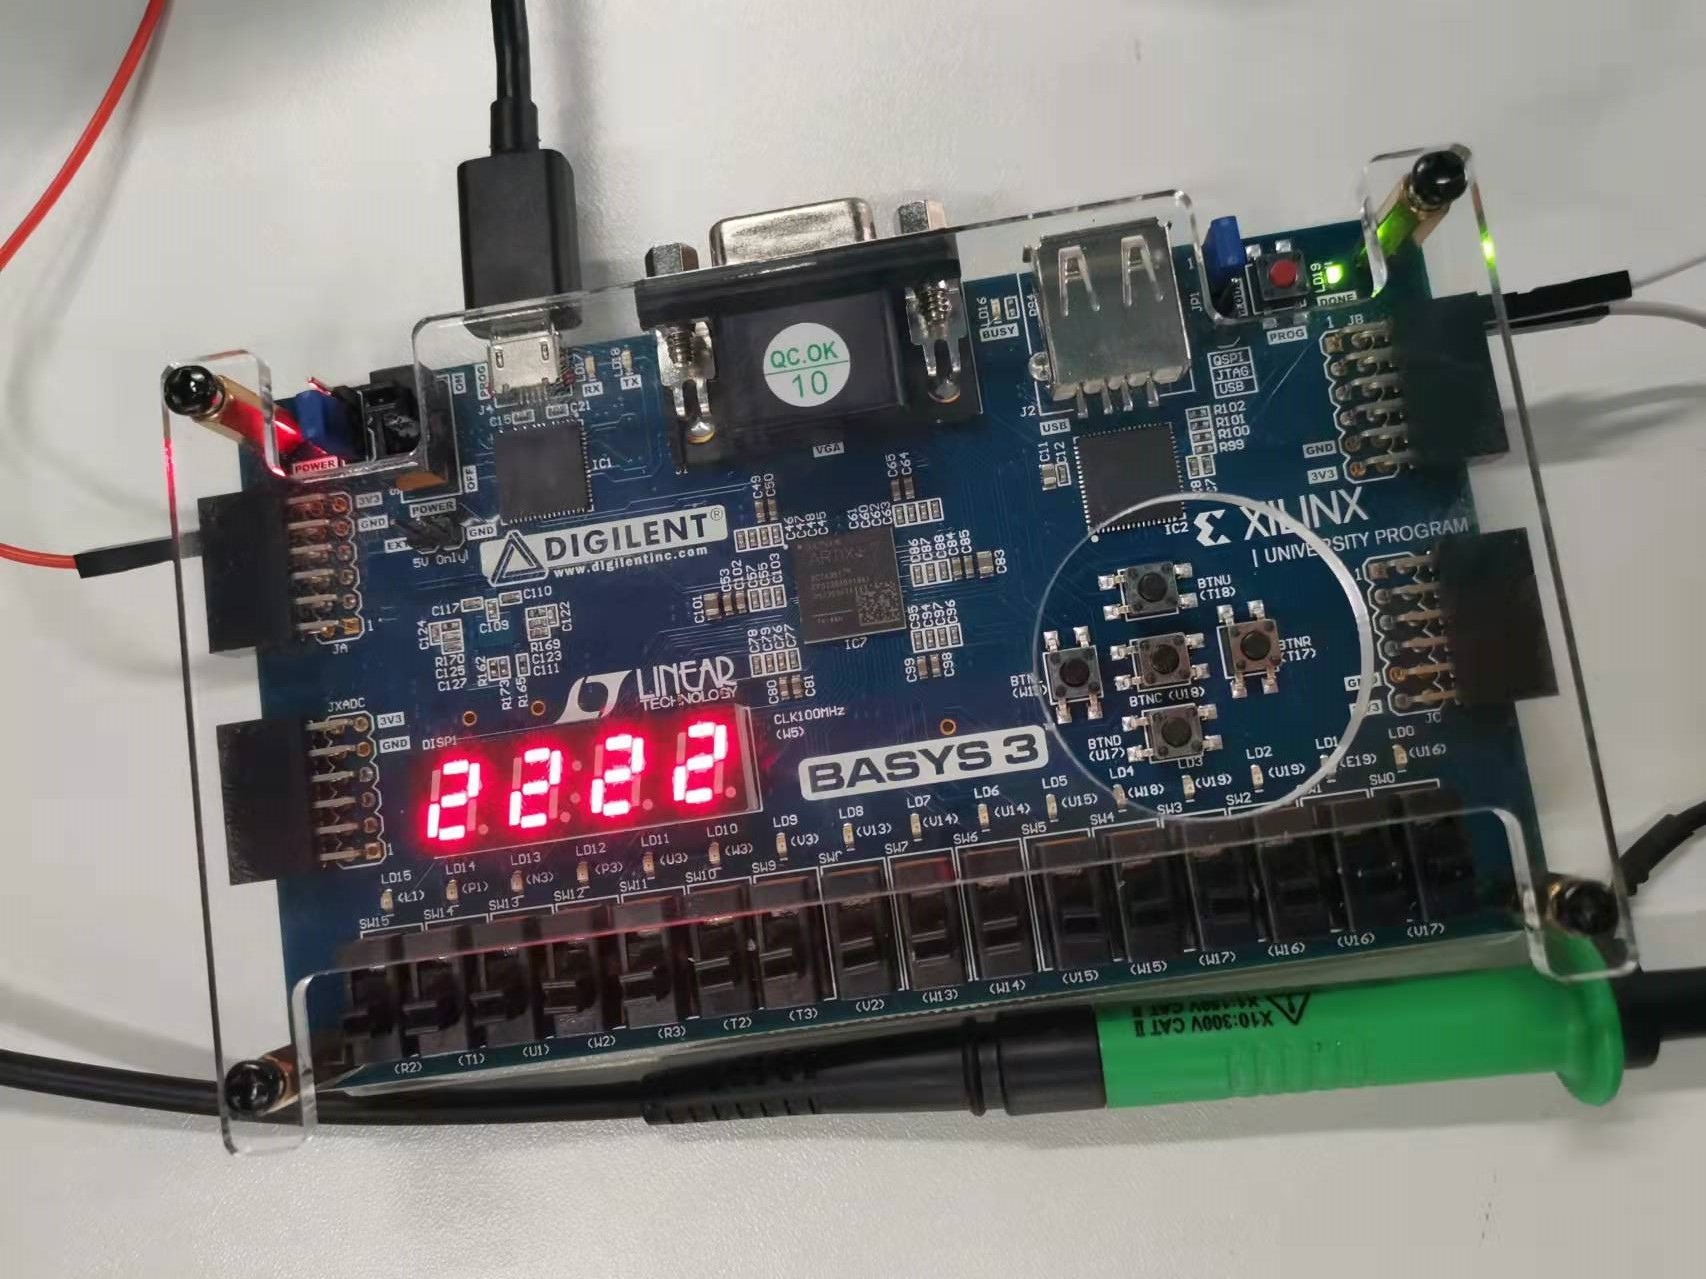
\includegraphics[width=0.3\textwidth]{original pic/2.jpg}}
    \subfigure[3]{
    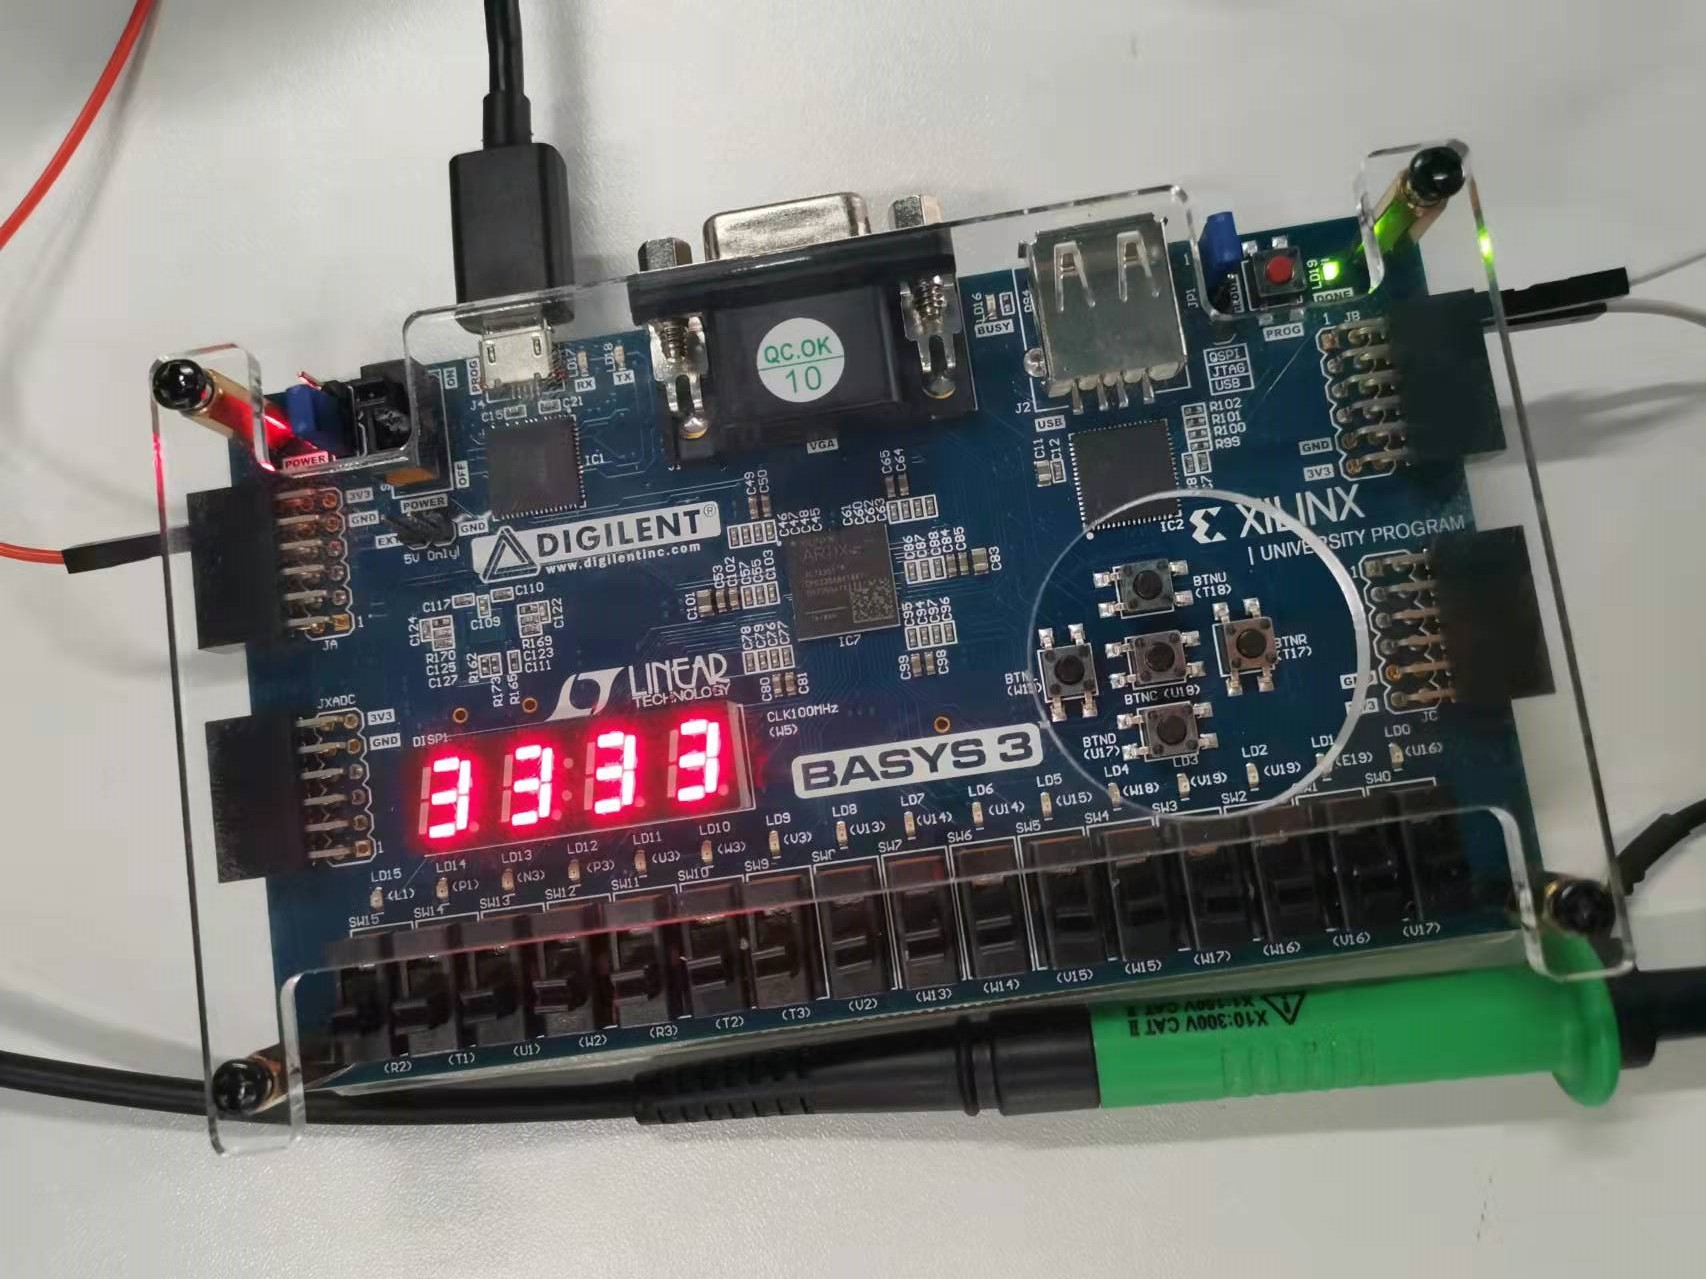
\includegraphics[width=0.3\textwidth]{original pic/3.jpg}}
    \subfigure[4]{
    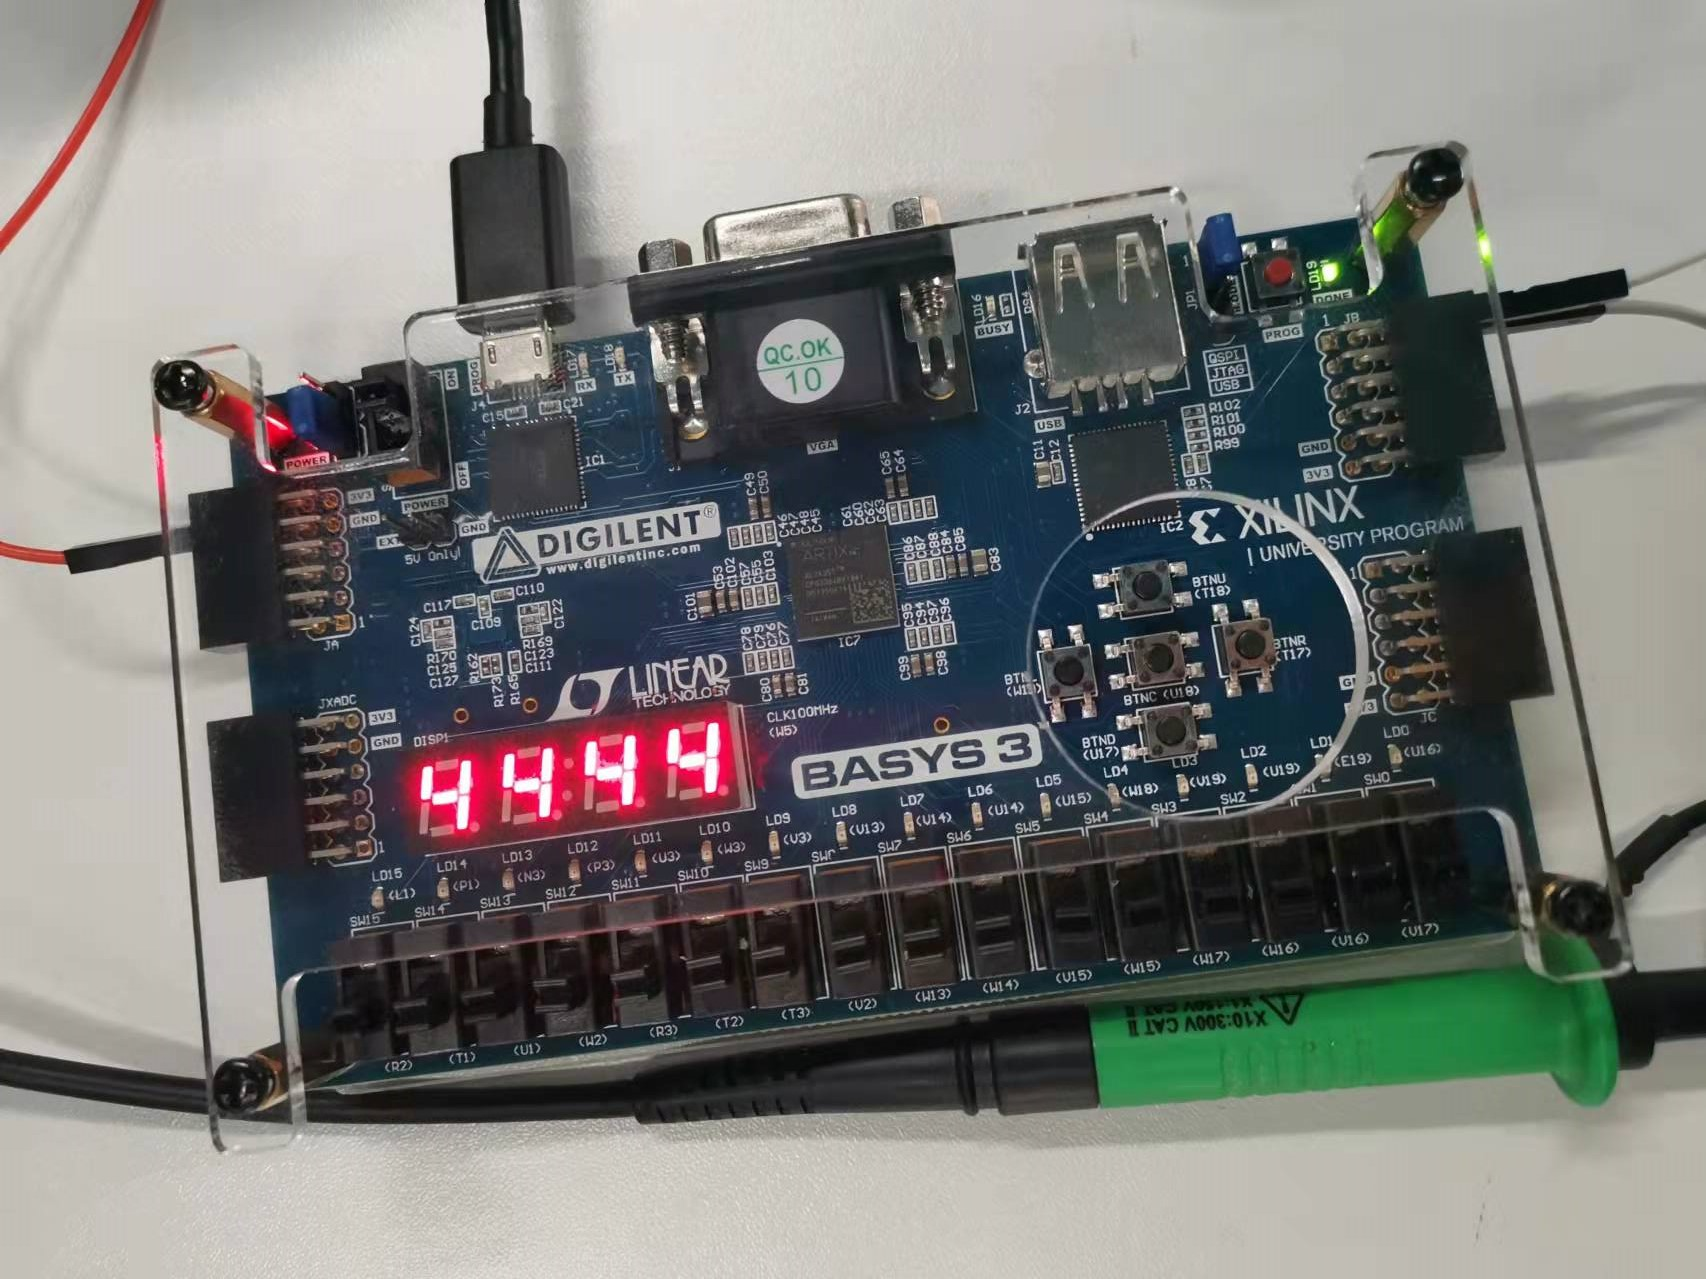
\includegraphics[width=0.3\textwidth]{original pic/4.jpg}}
    \subfigure[5]{
    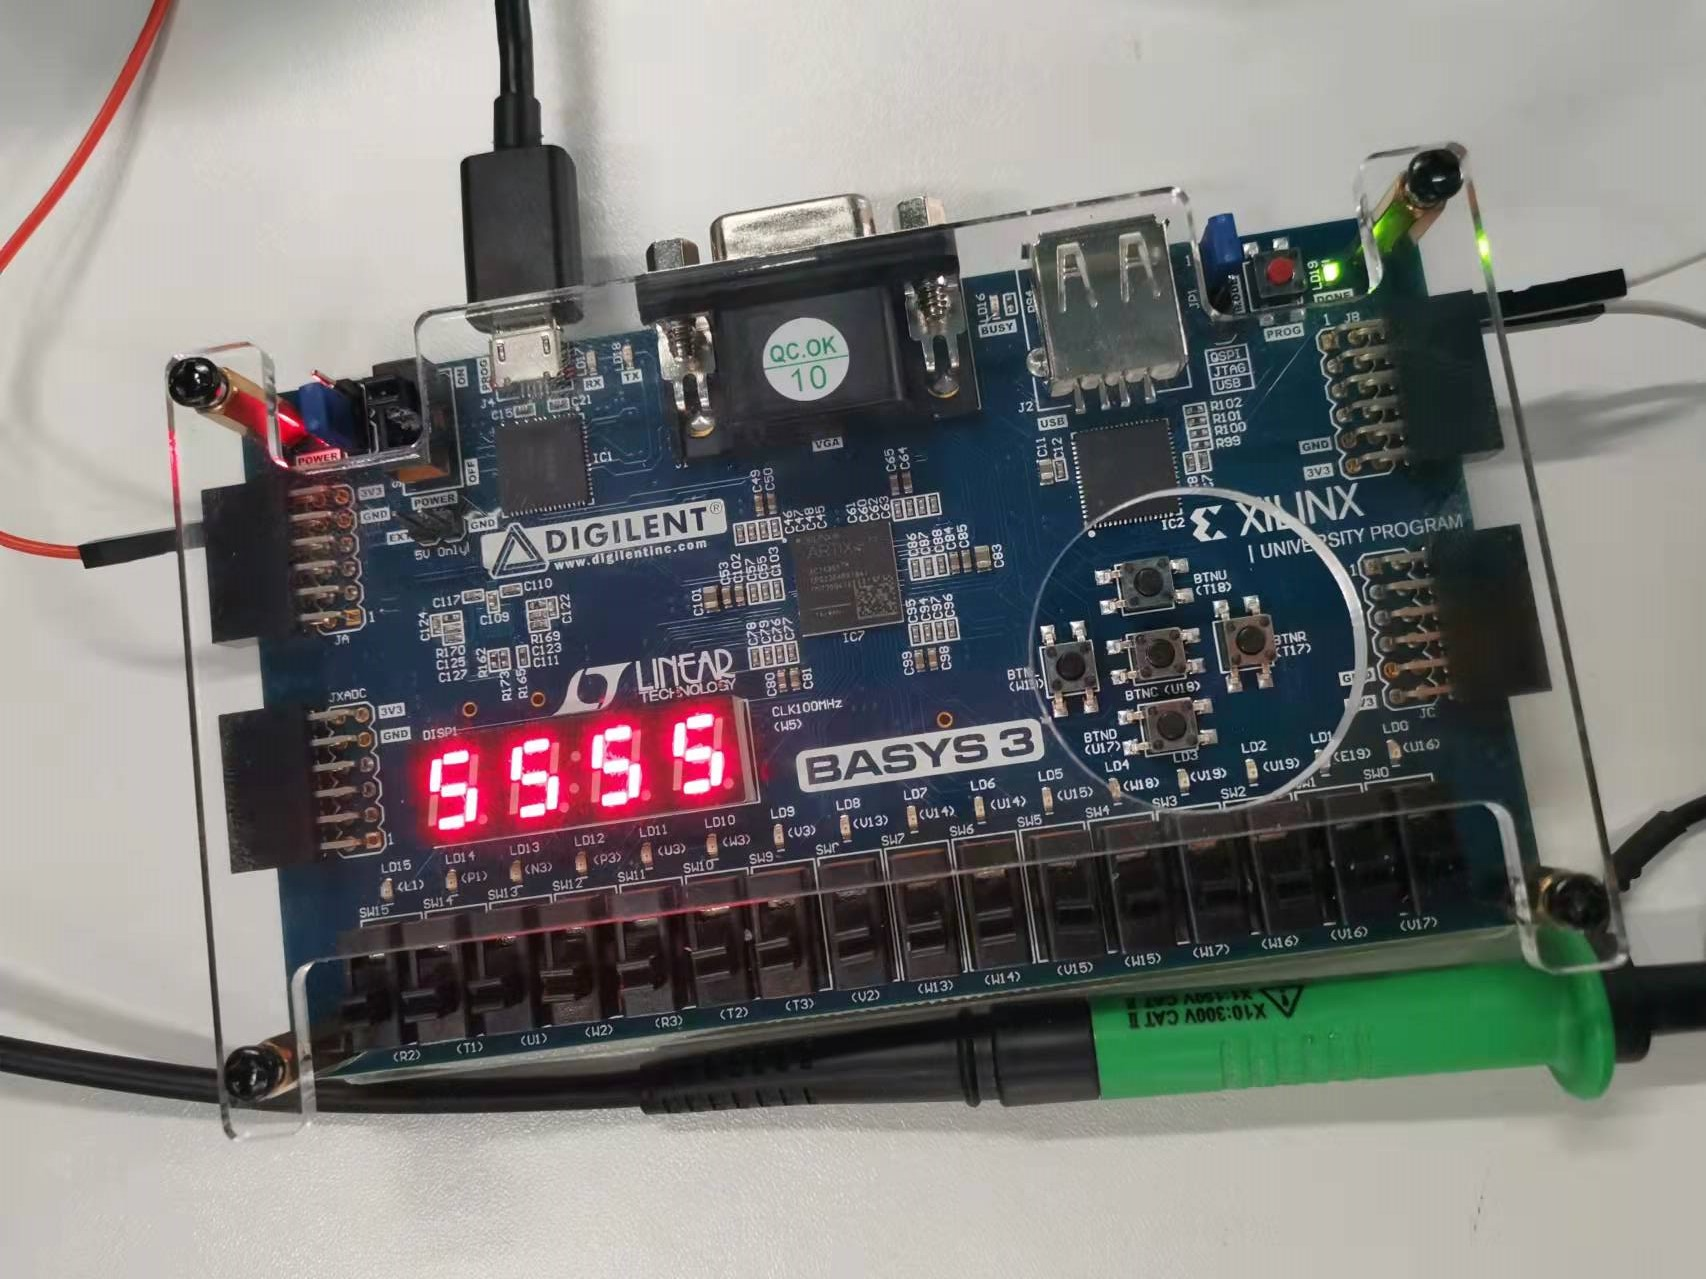
\includegraphics[width=0.3\textwidth]{original pic/5.jpg}}
    \subfigure[6]{
    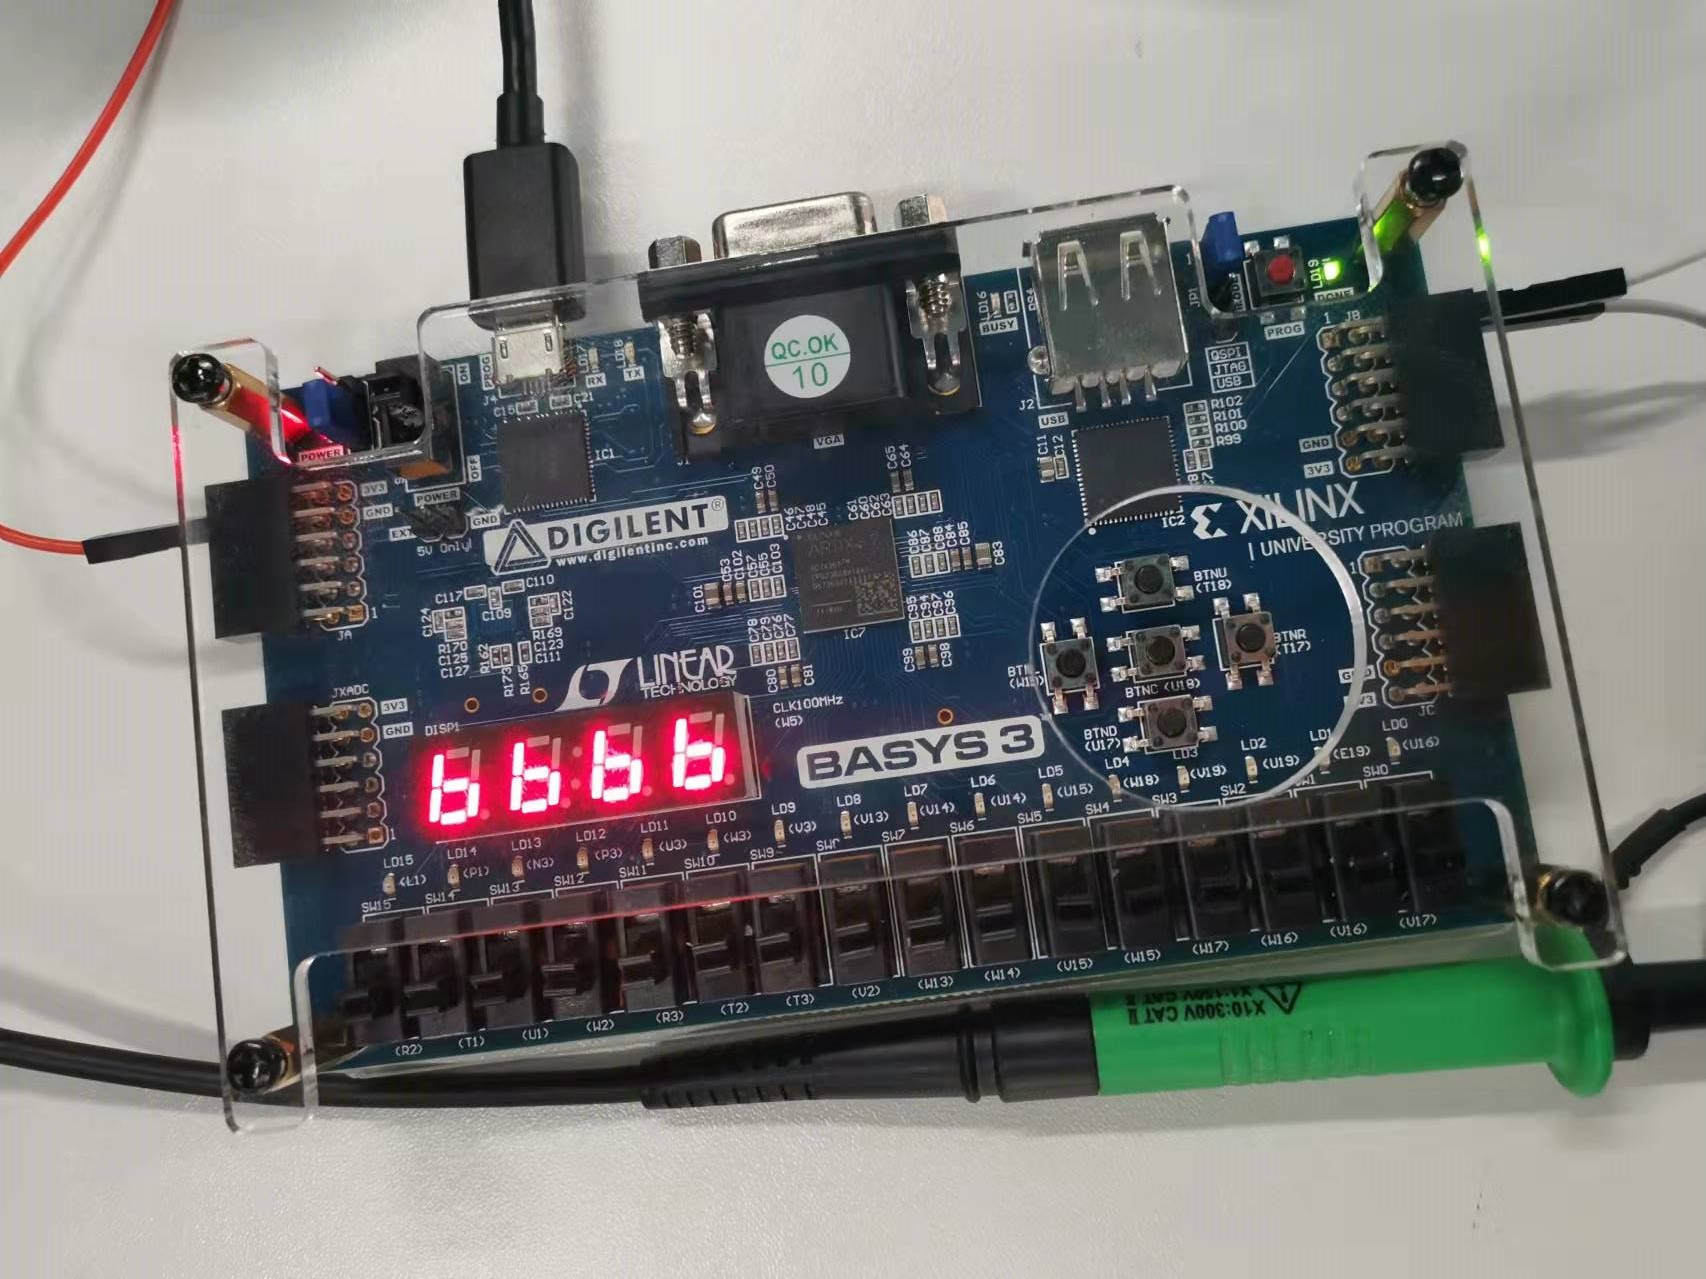
\includegraphics[width=0.3\textwidth]{original pic/6.jpg}}
    \subfigure[7]{
    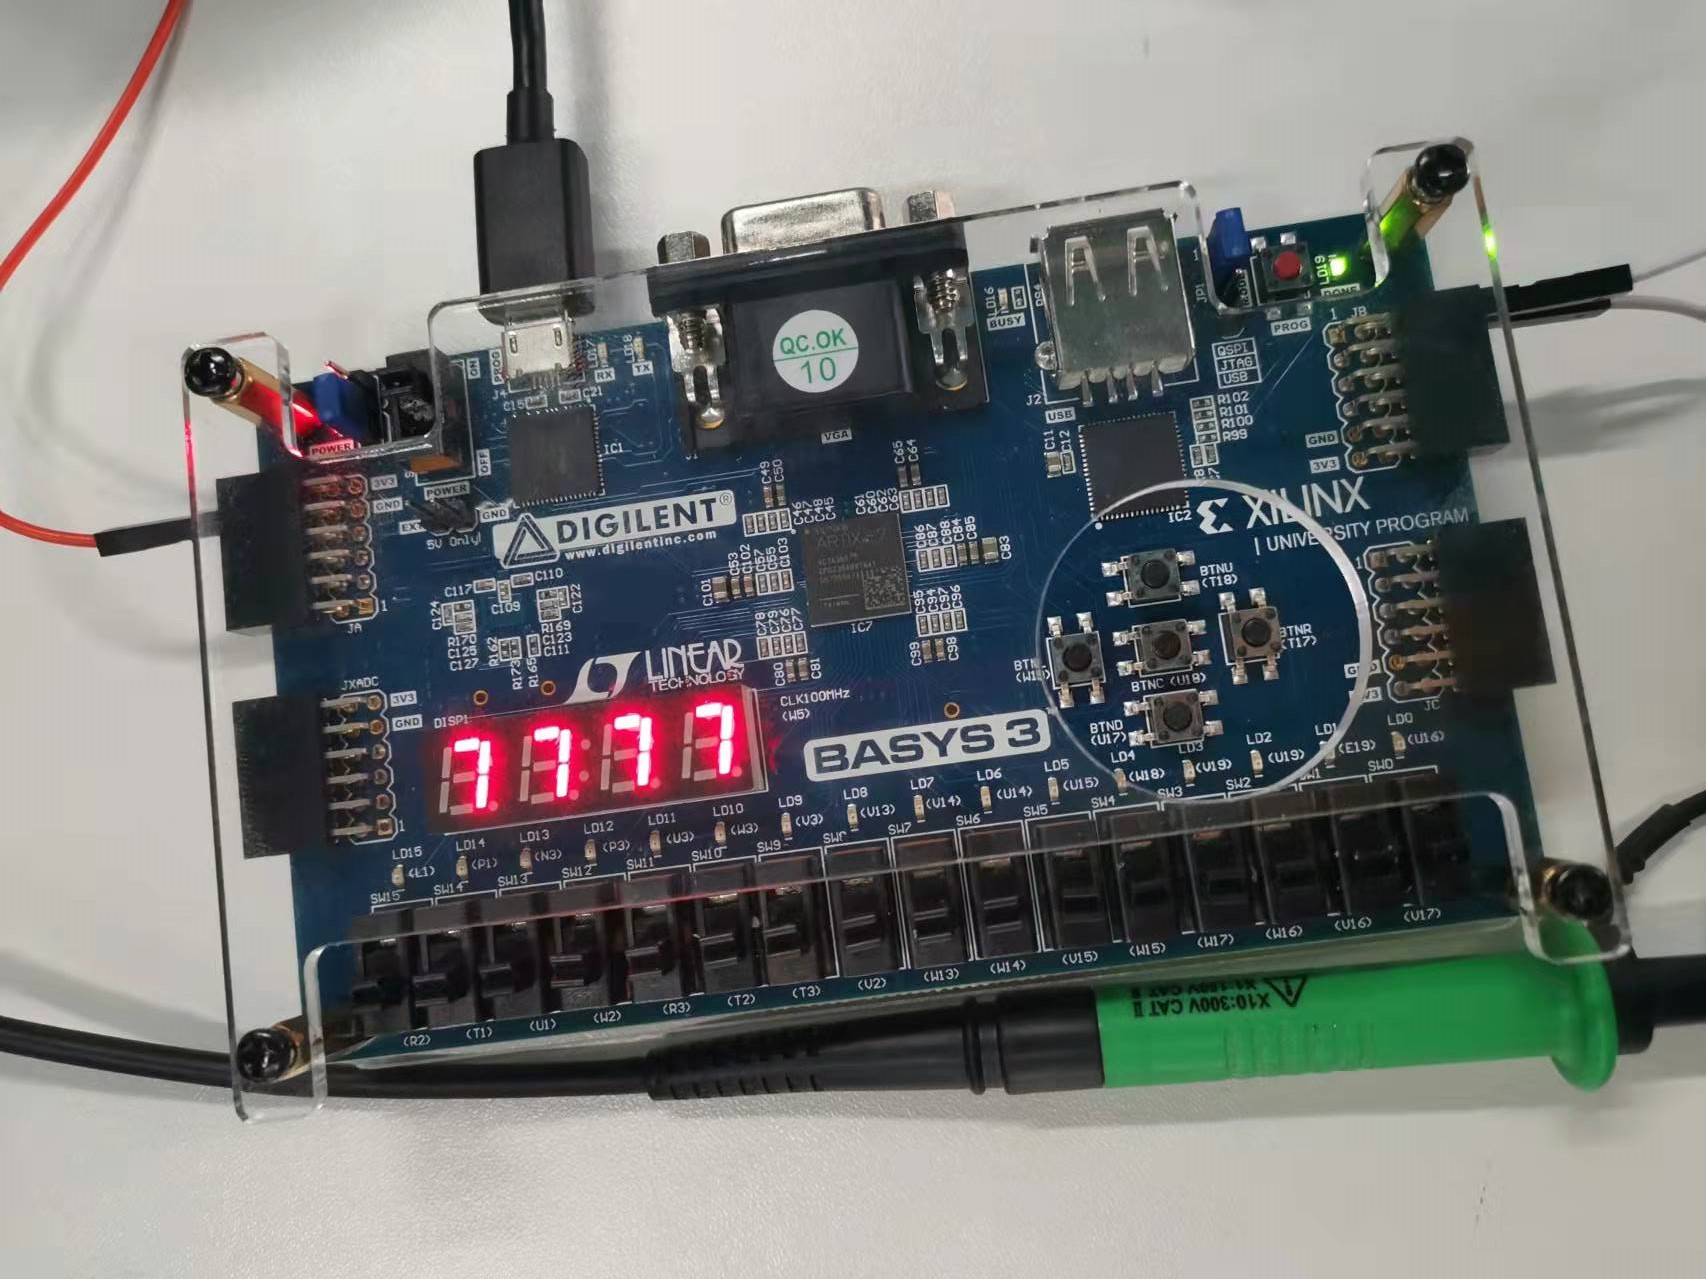
\includegraphics[width=0.3\textwidth]{original pic/7.jpg}}
    \subfigure[8]{
    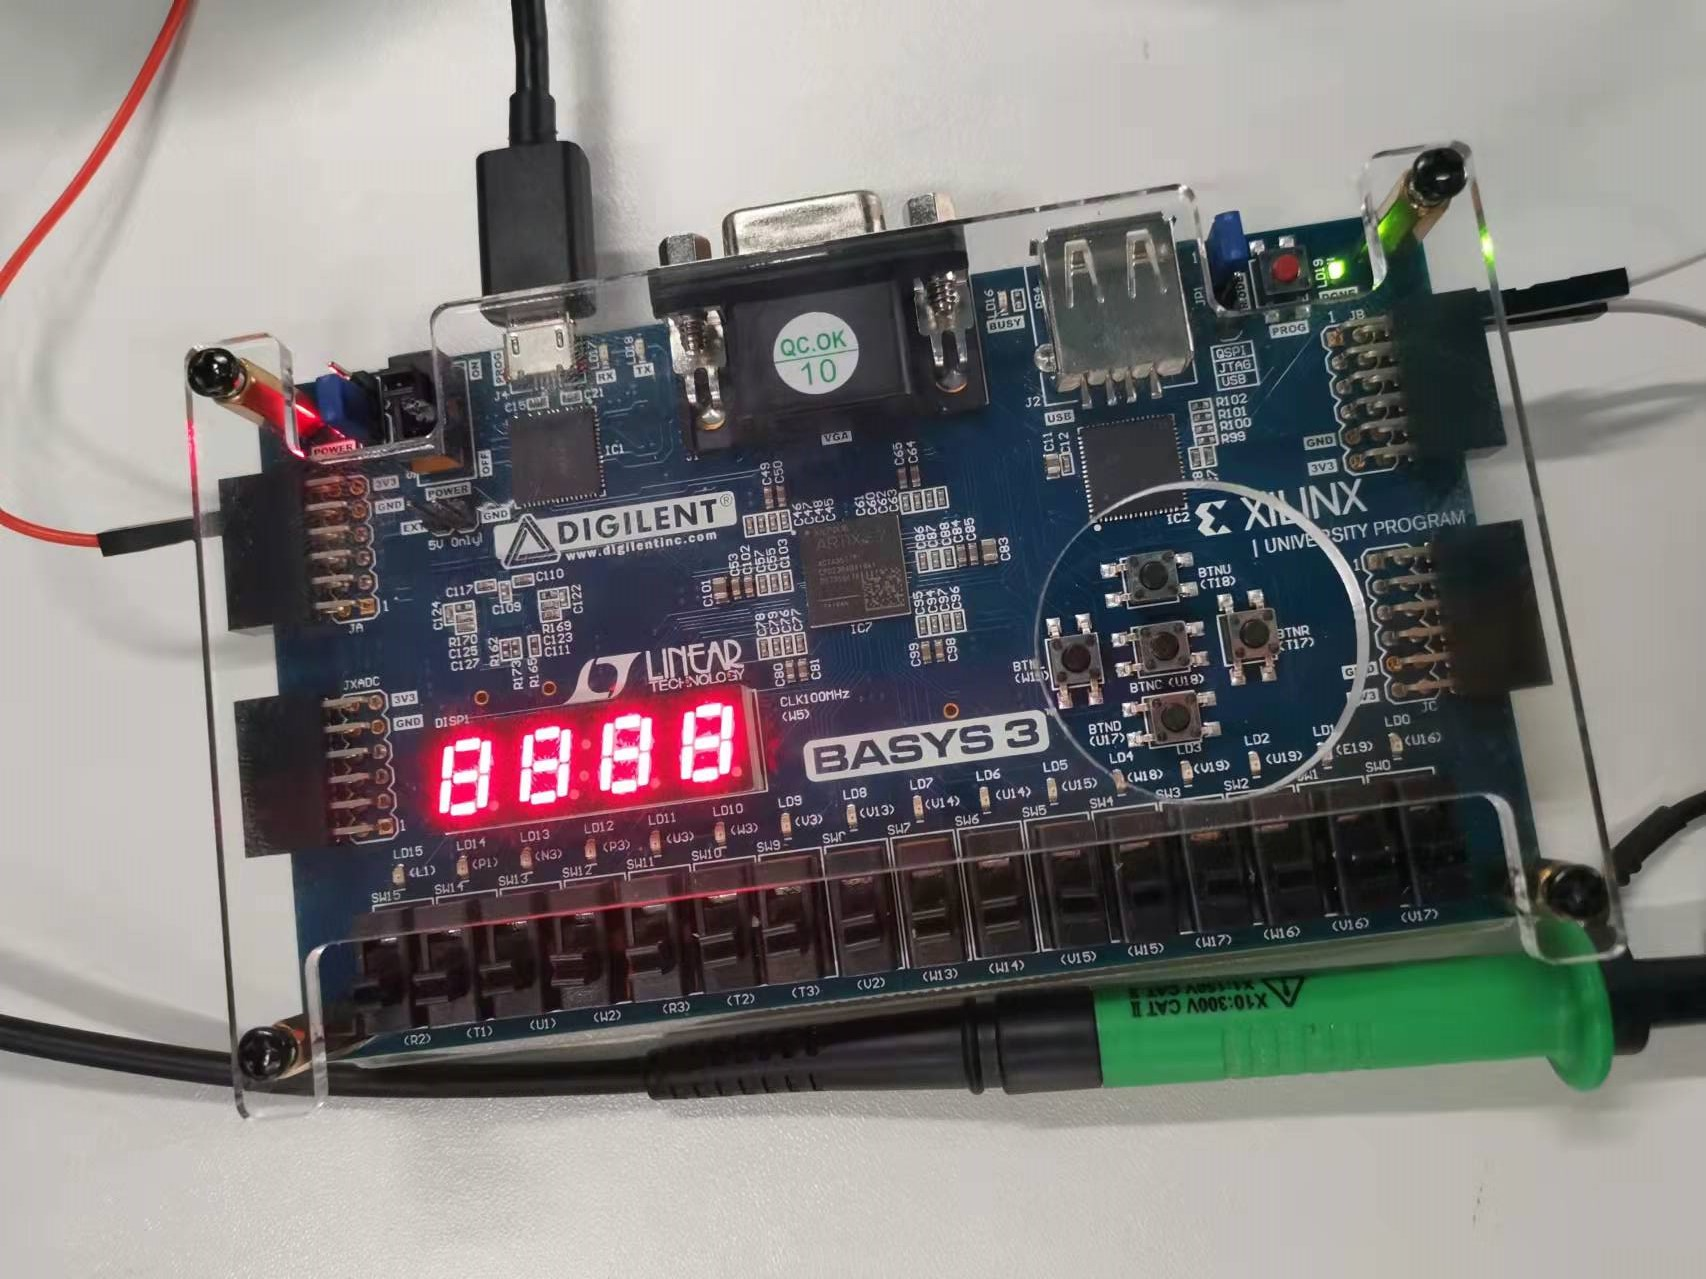
\includegraphics[width=0.3\textwidth]{original pic/8.jpg}}
    \subfigure[9]{
    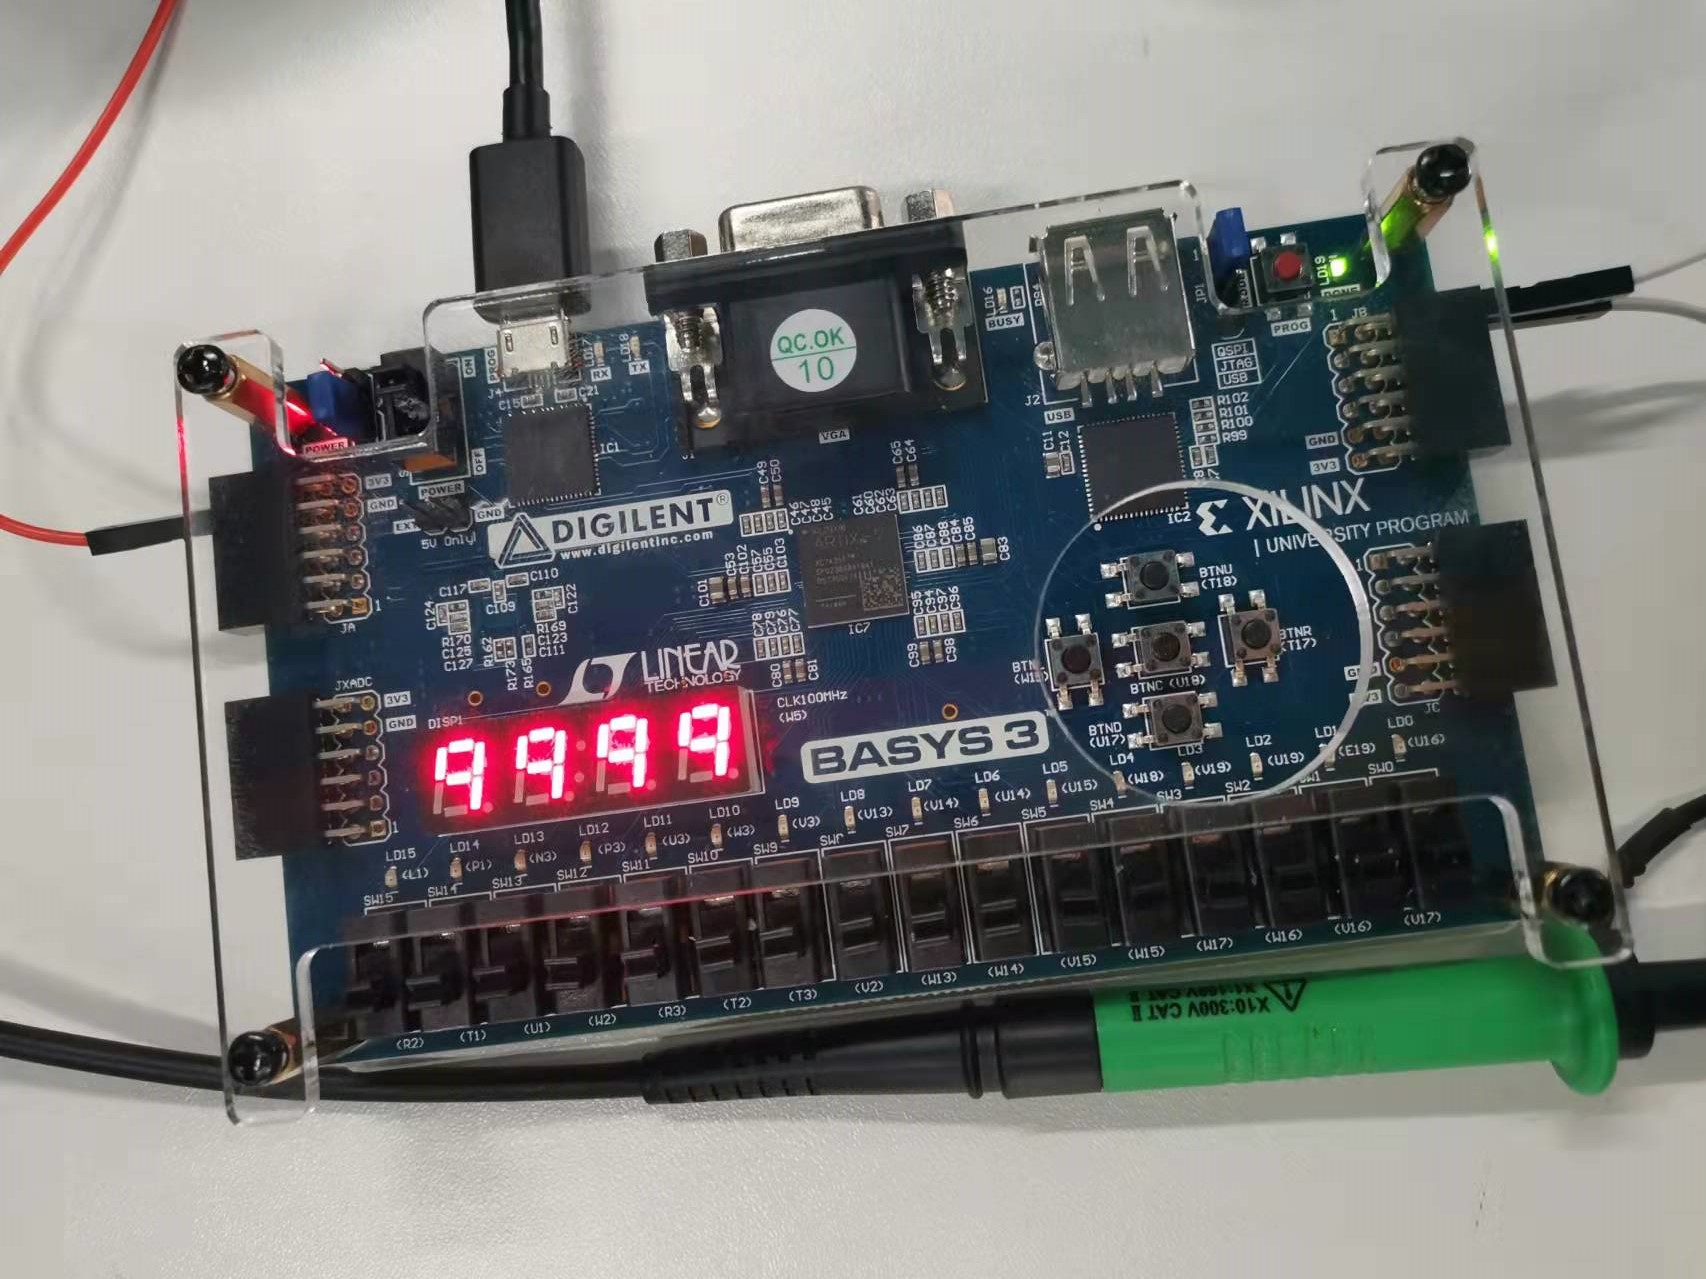
\includegraphics[width=0.3\textwidth]{original pic/9.jpg}}
    
    \caption{十进制计数器数码管显示}
    \label{10counter_slow}
\end{figure}

\(SW_0 =0 ,  SW_1 = 1\)时,时钟周期为\SI{3}{\kHz},数码管由于视觉暂留现象全亮,此时使用示波器观察计数器各输出引脚波形如图\ref{10counter_fast}所示。可以看出,在计数器一个全周期内共经历了10个时钟周期,与十进制计数器要求相符。

\begin{figure}[H]
    \centering
    \subfigure[\(JB_1\)]{
    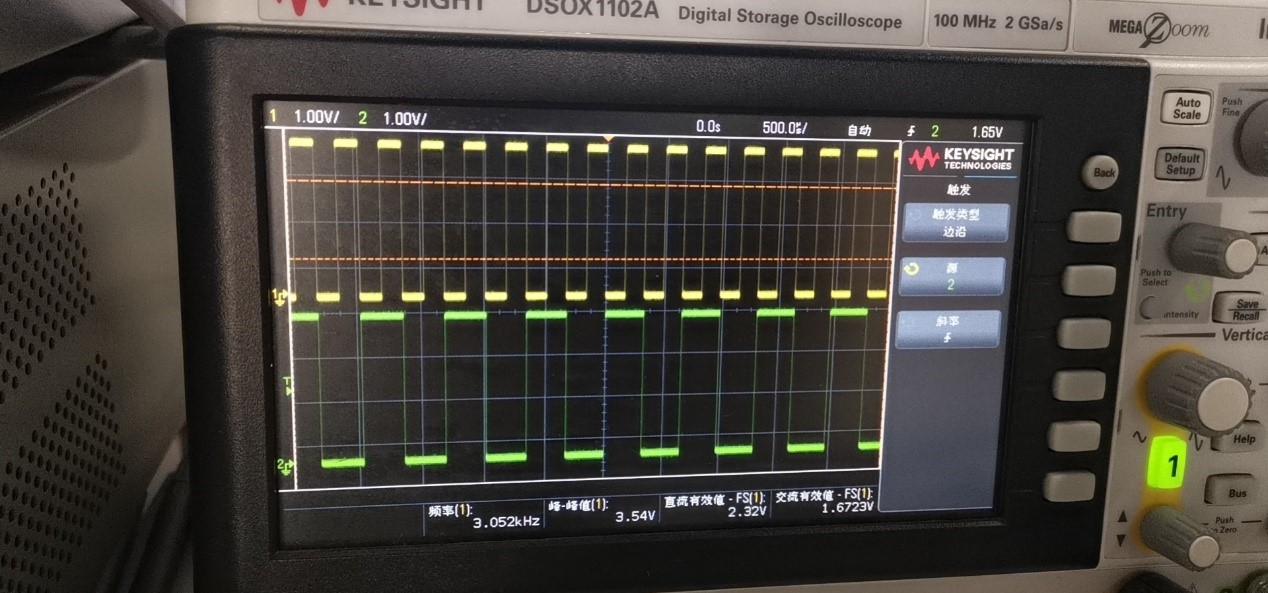
\includegraphics[width=0.45\textwidth]{10/jb1.jpg}}
    \subfigure[\(JB_2\)]{
    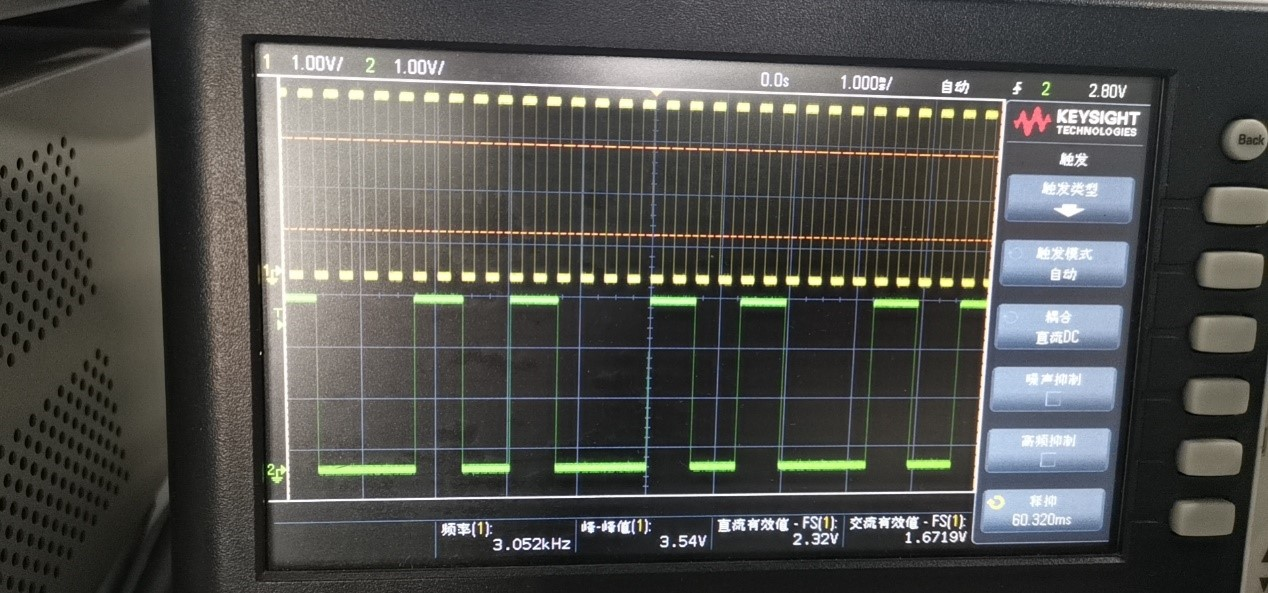
\includegraphics[width=0.45\textwidth]{10/jb2.jpg}}
    \subfigure[\(JB_3\)]{
    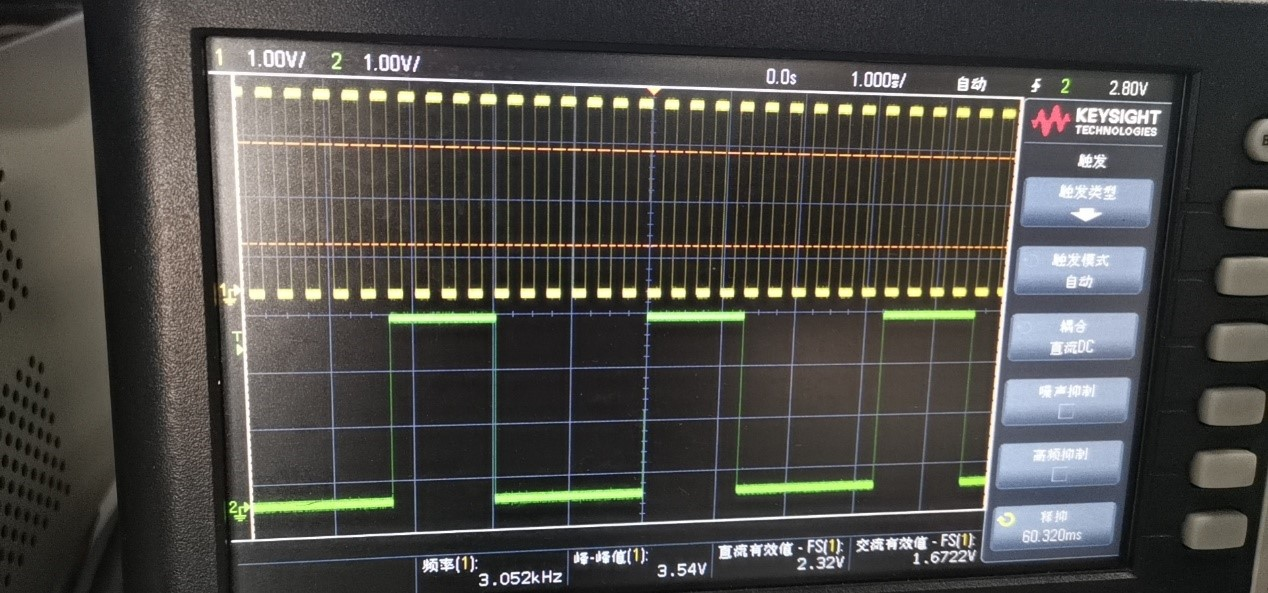
\includegraphics[width=0.45\textwidth]{10/jb3.jpg}}
    \subfigure[\(JB_4\)]{
    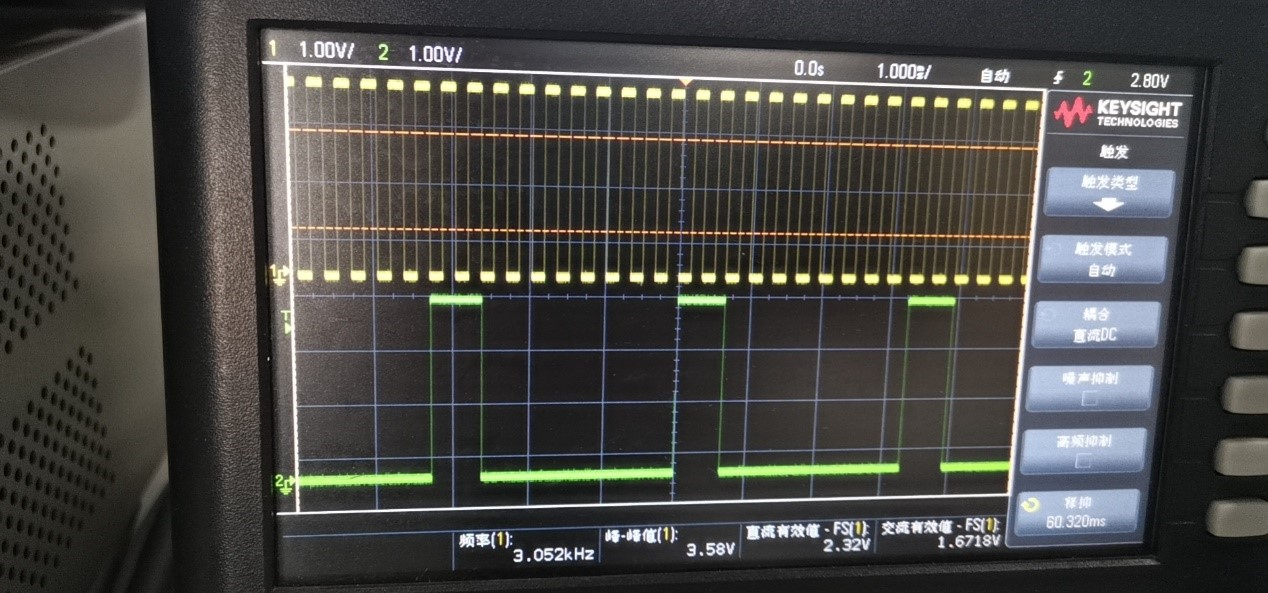
\includegraphics[width=0.45\textwidth]{10/jb4.jpg}}

    
    \caption{十进制计数器引脚输出波形}
    \label{10counter_fast}
\end{figure}

\subsubsection{小结}
\begin{itemize}
    \item 观察了十进制计数器连接数码管可以实现\(0 \sim 9\)数字循环显示的功能。
    \item 测量了十进制计数器的输出波形,符合10个时钟周期1循环的要求。
\end{itemize}

\subsection{16进制加法计数器}
开发板连接至电脑后下载已经编译好的16进制计数器bit流文件。
\par 将\(SW_0\)拨至闭合位置、\(SW_1\)拨至断开位置,观察计数器数字缓慢变化。将\(SW_1\)闭合,使用示波器观察计数器各输出引脚波形。
\subsubsection{实验结果}
\(SW_0 =1, SW_1 = 0\)时,时钟周期为\SI{0.75}{\Hz},计数器数字缓慢变化。观察到十进制计数器共有10个稳态,分别显示数字\(0\sim 9\),以及\(10\sim 15\)所对应输出数码,如图\ref{16counter_slow}所示。

\begin{figure}[H]
    \centering
    \subfigure[0]{
    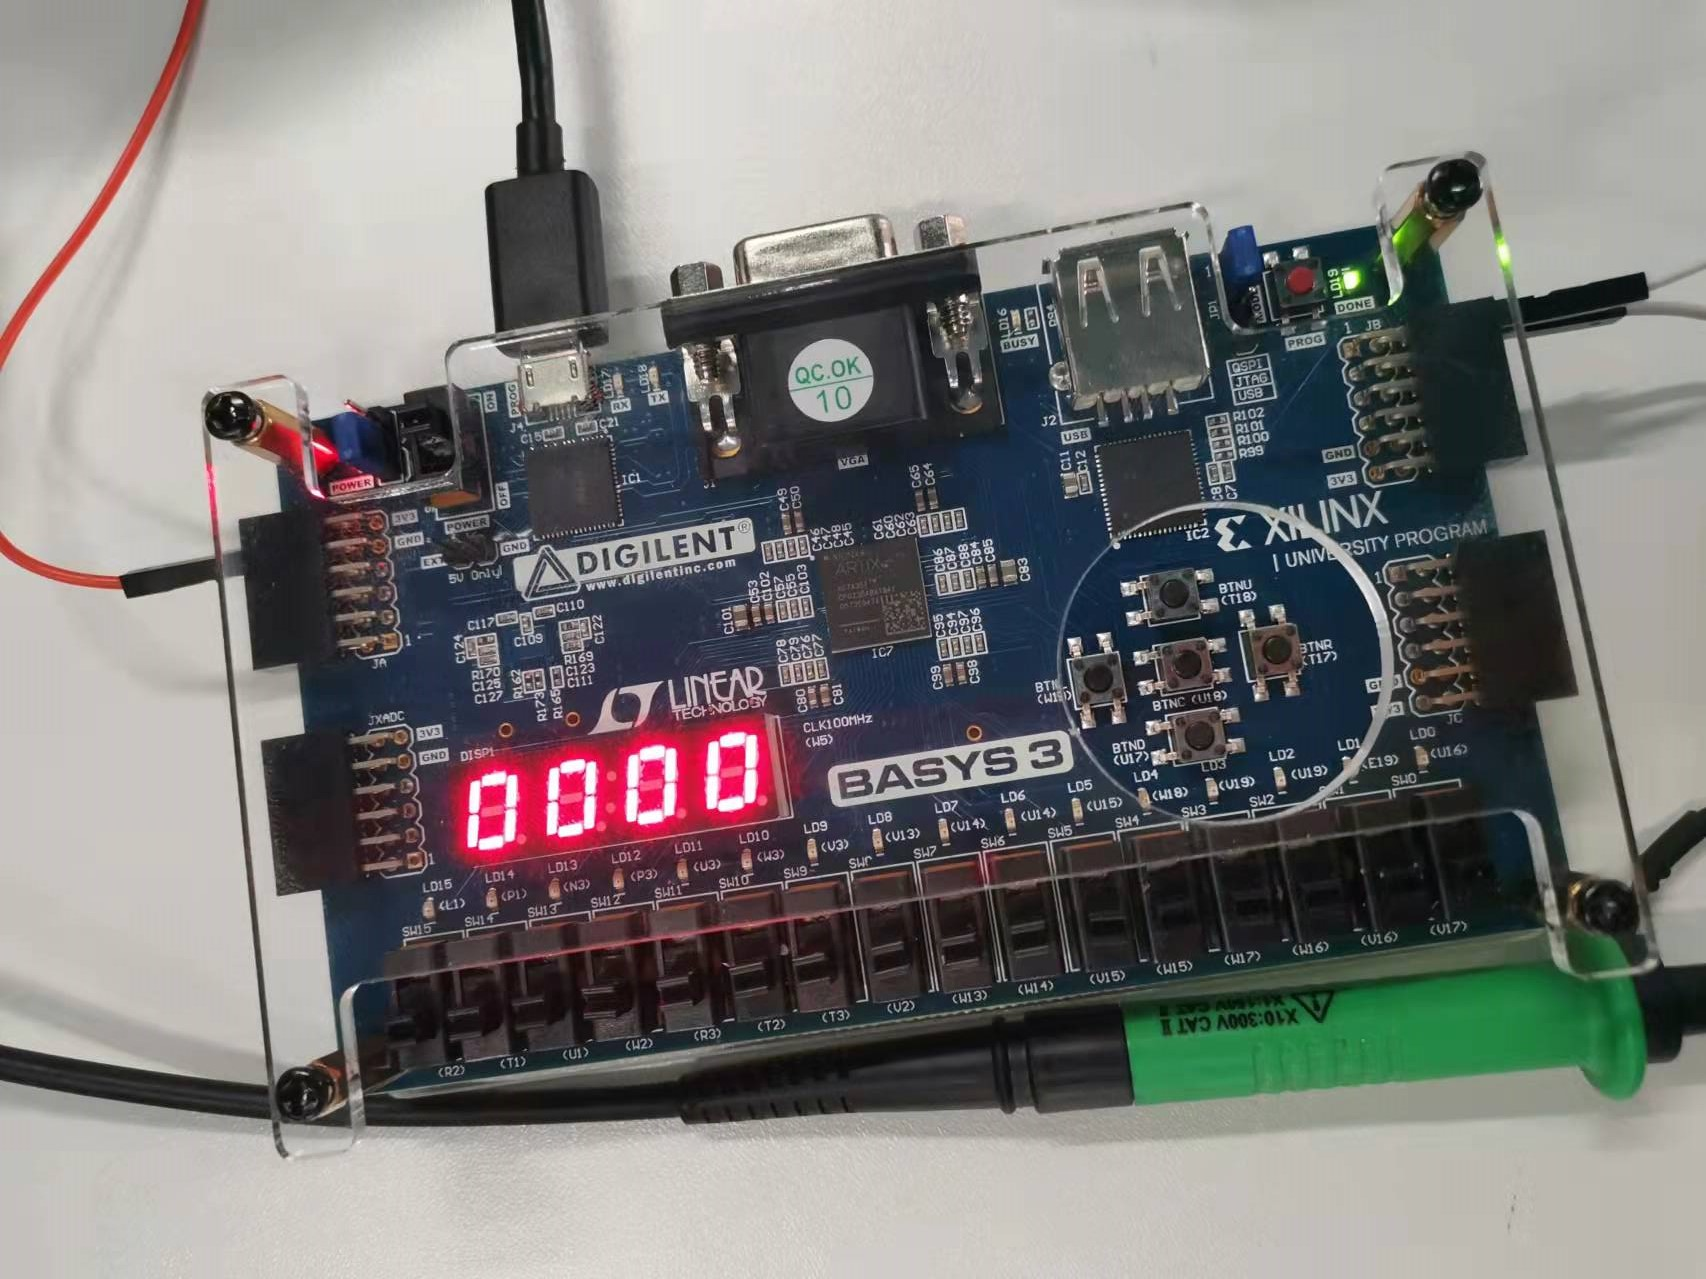
\includegraphics[width=0.22\textwidth]{original pic/0.jpg}}
    \subfigure[1]{
    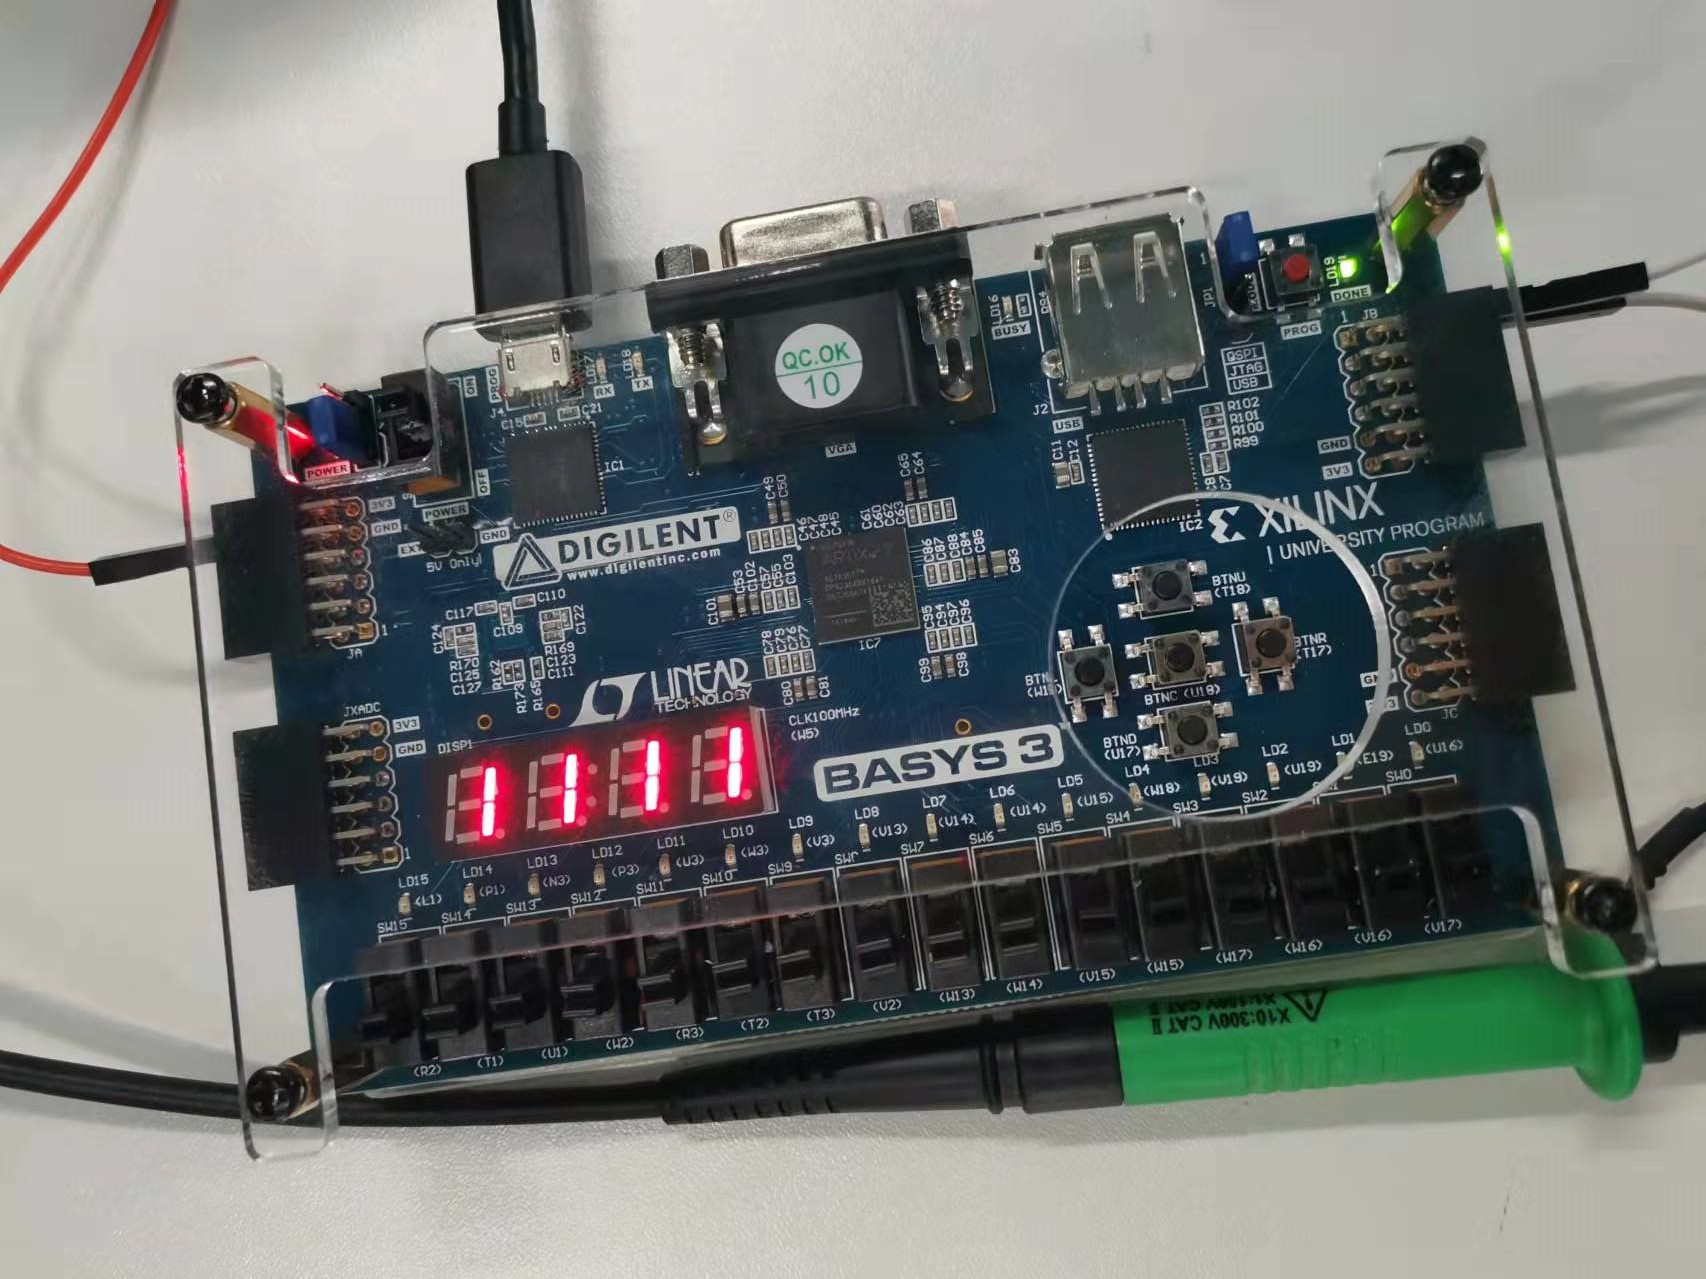
\includegraphics[width=0.22\textwidth]{original pic/1.jpg}}
    \subfigure[2]{
    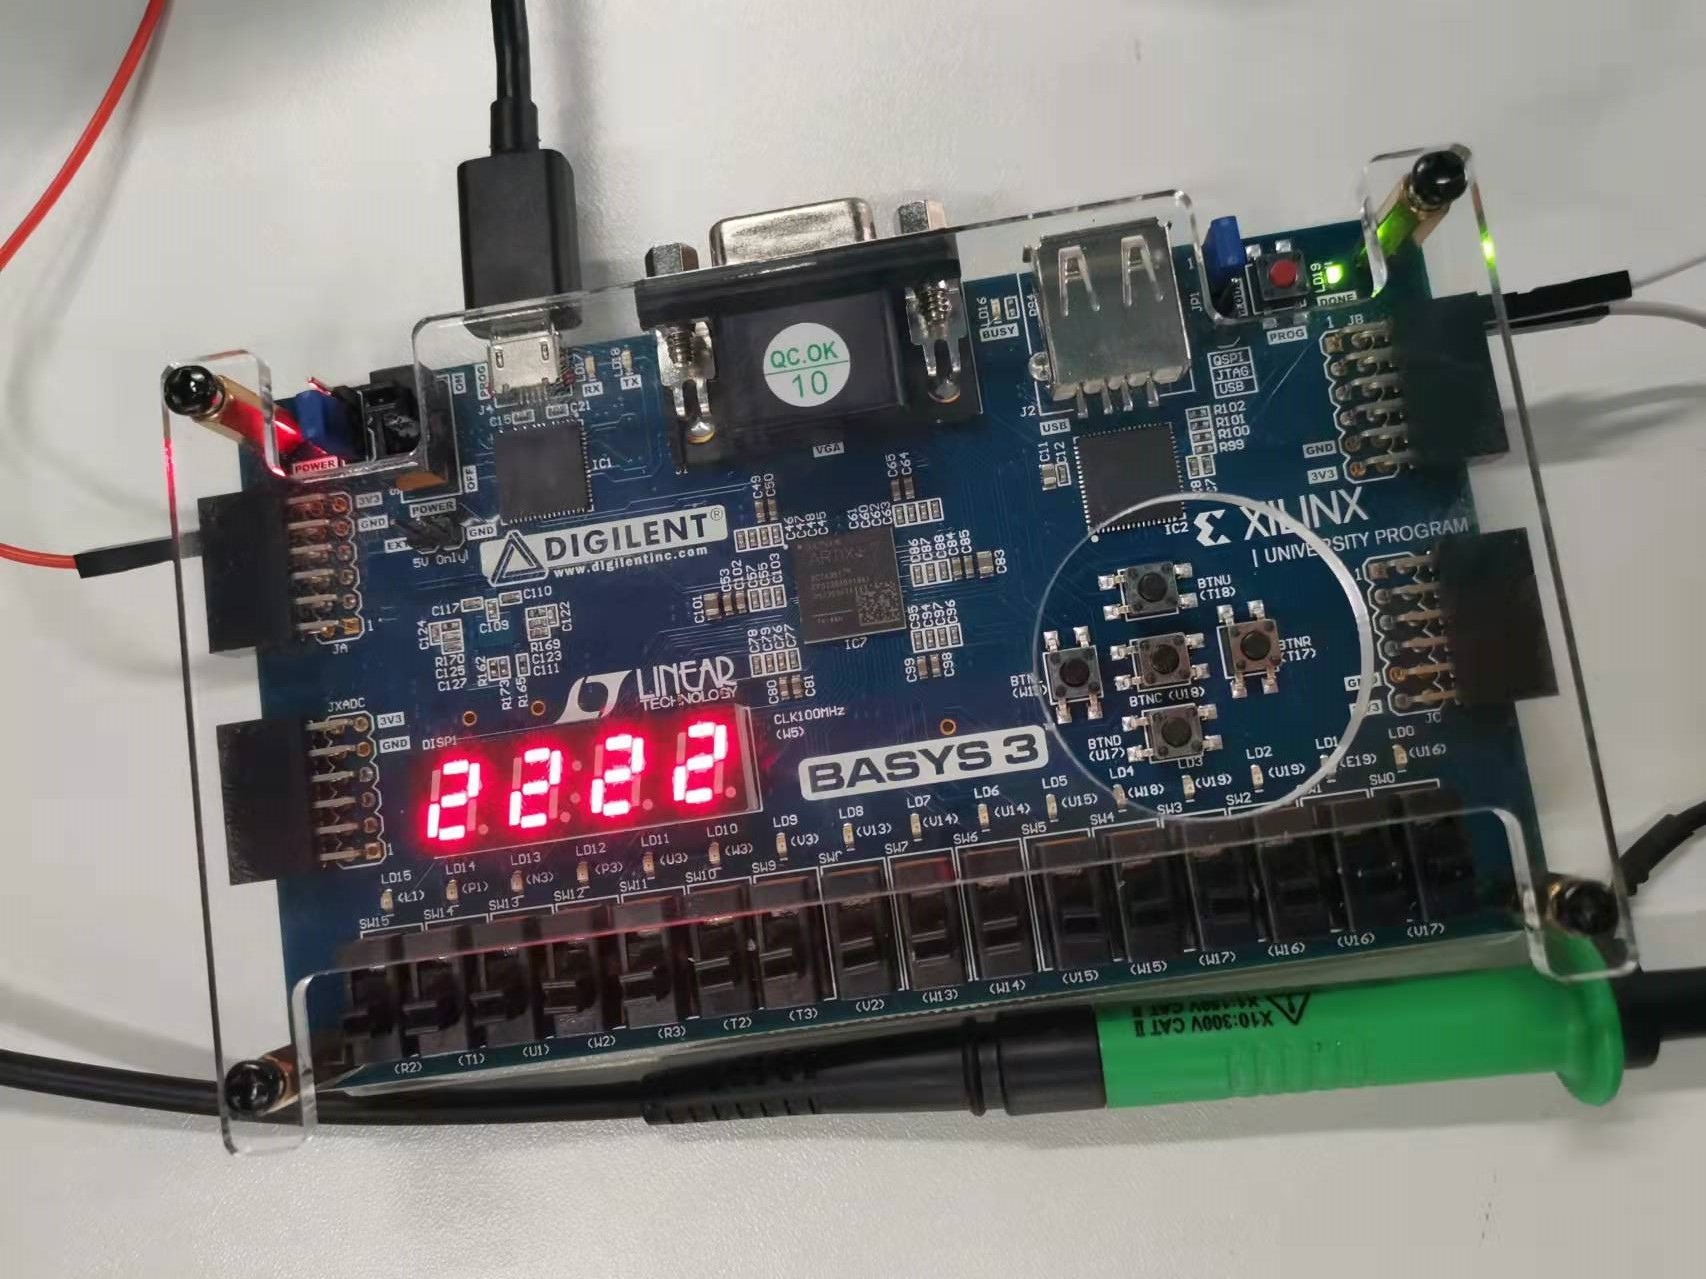
\includegraphics[width=0.22\textwidth]{original pic/2.jpg}}
    \subfigure[3]{
    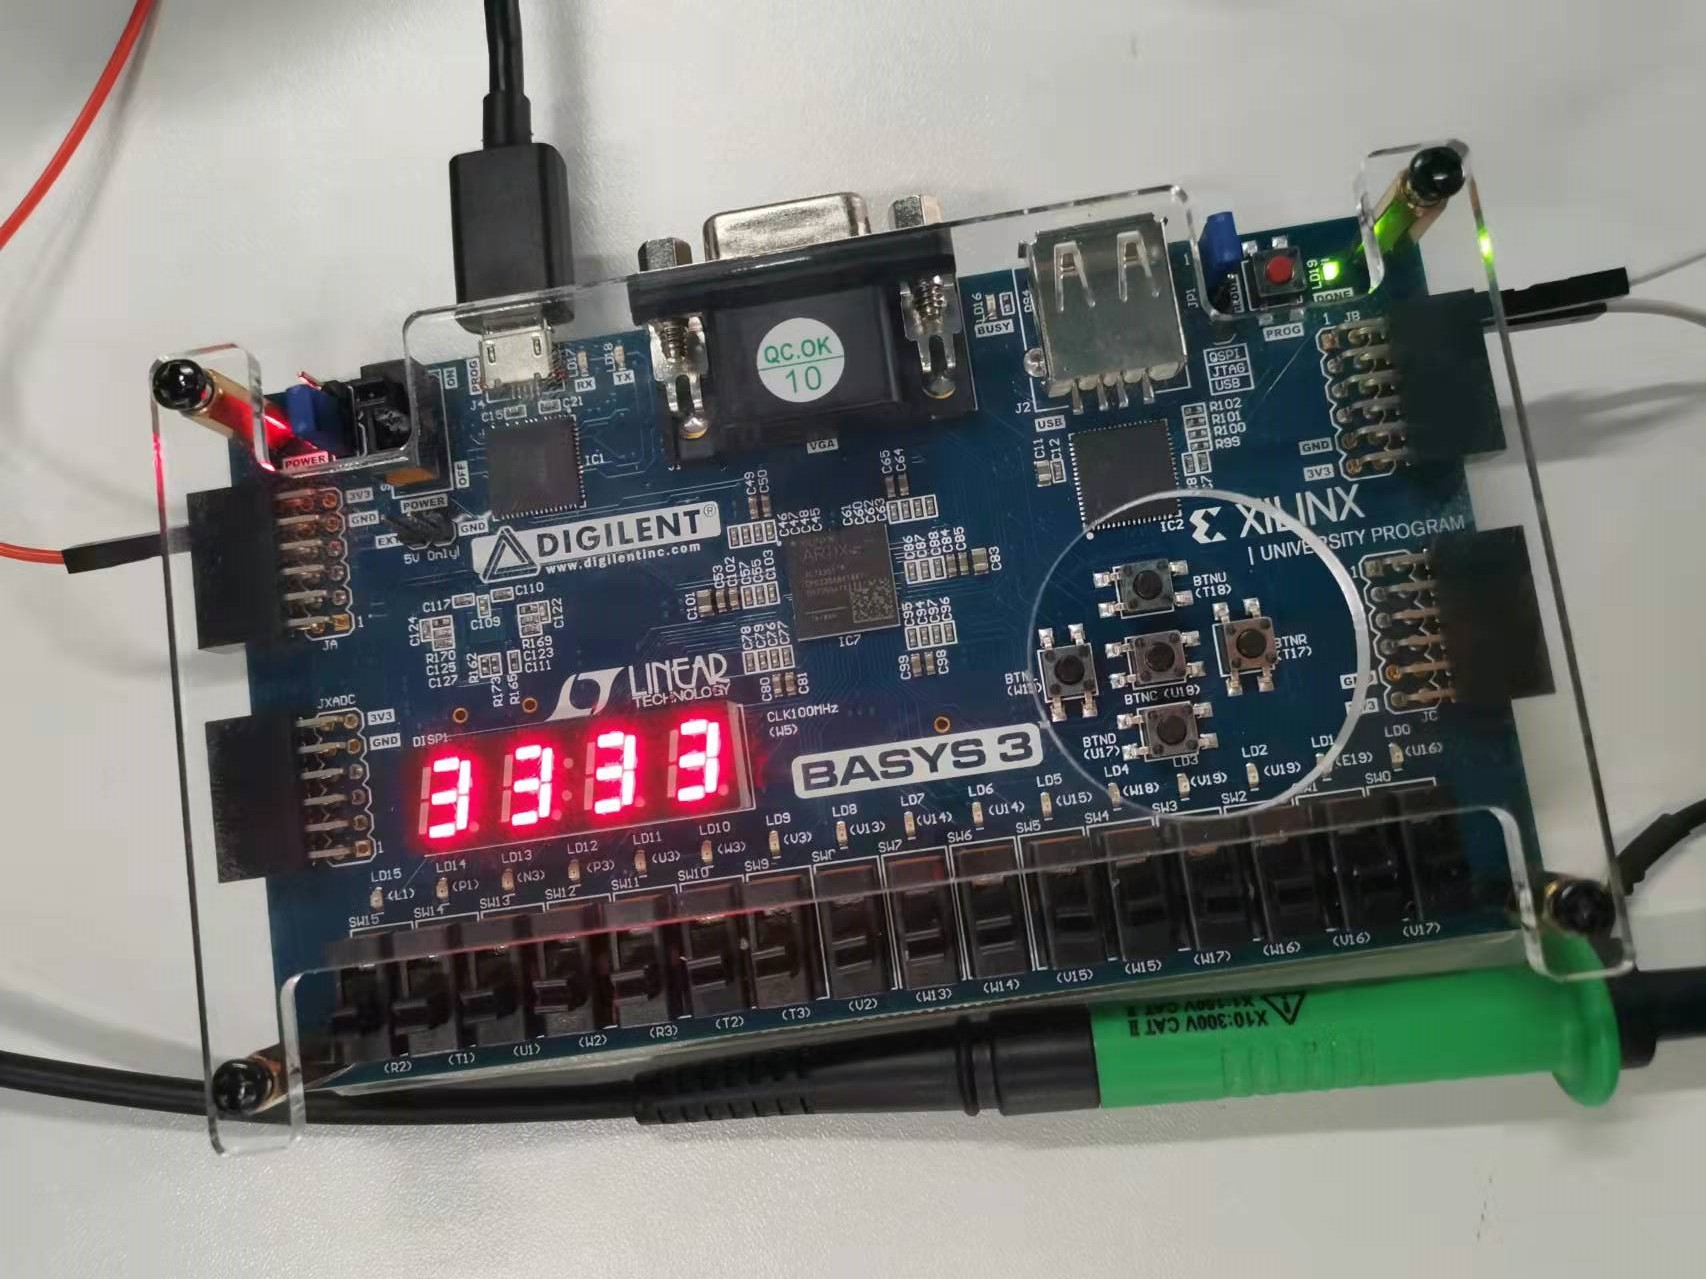
\includegraphics[width=0.22\textwidth]{original pic/3.jpg}}
    \subfigure[4]{
    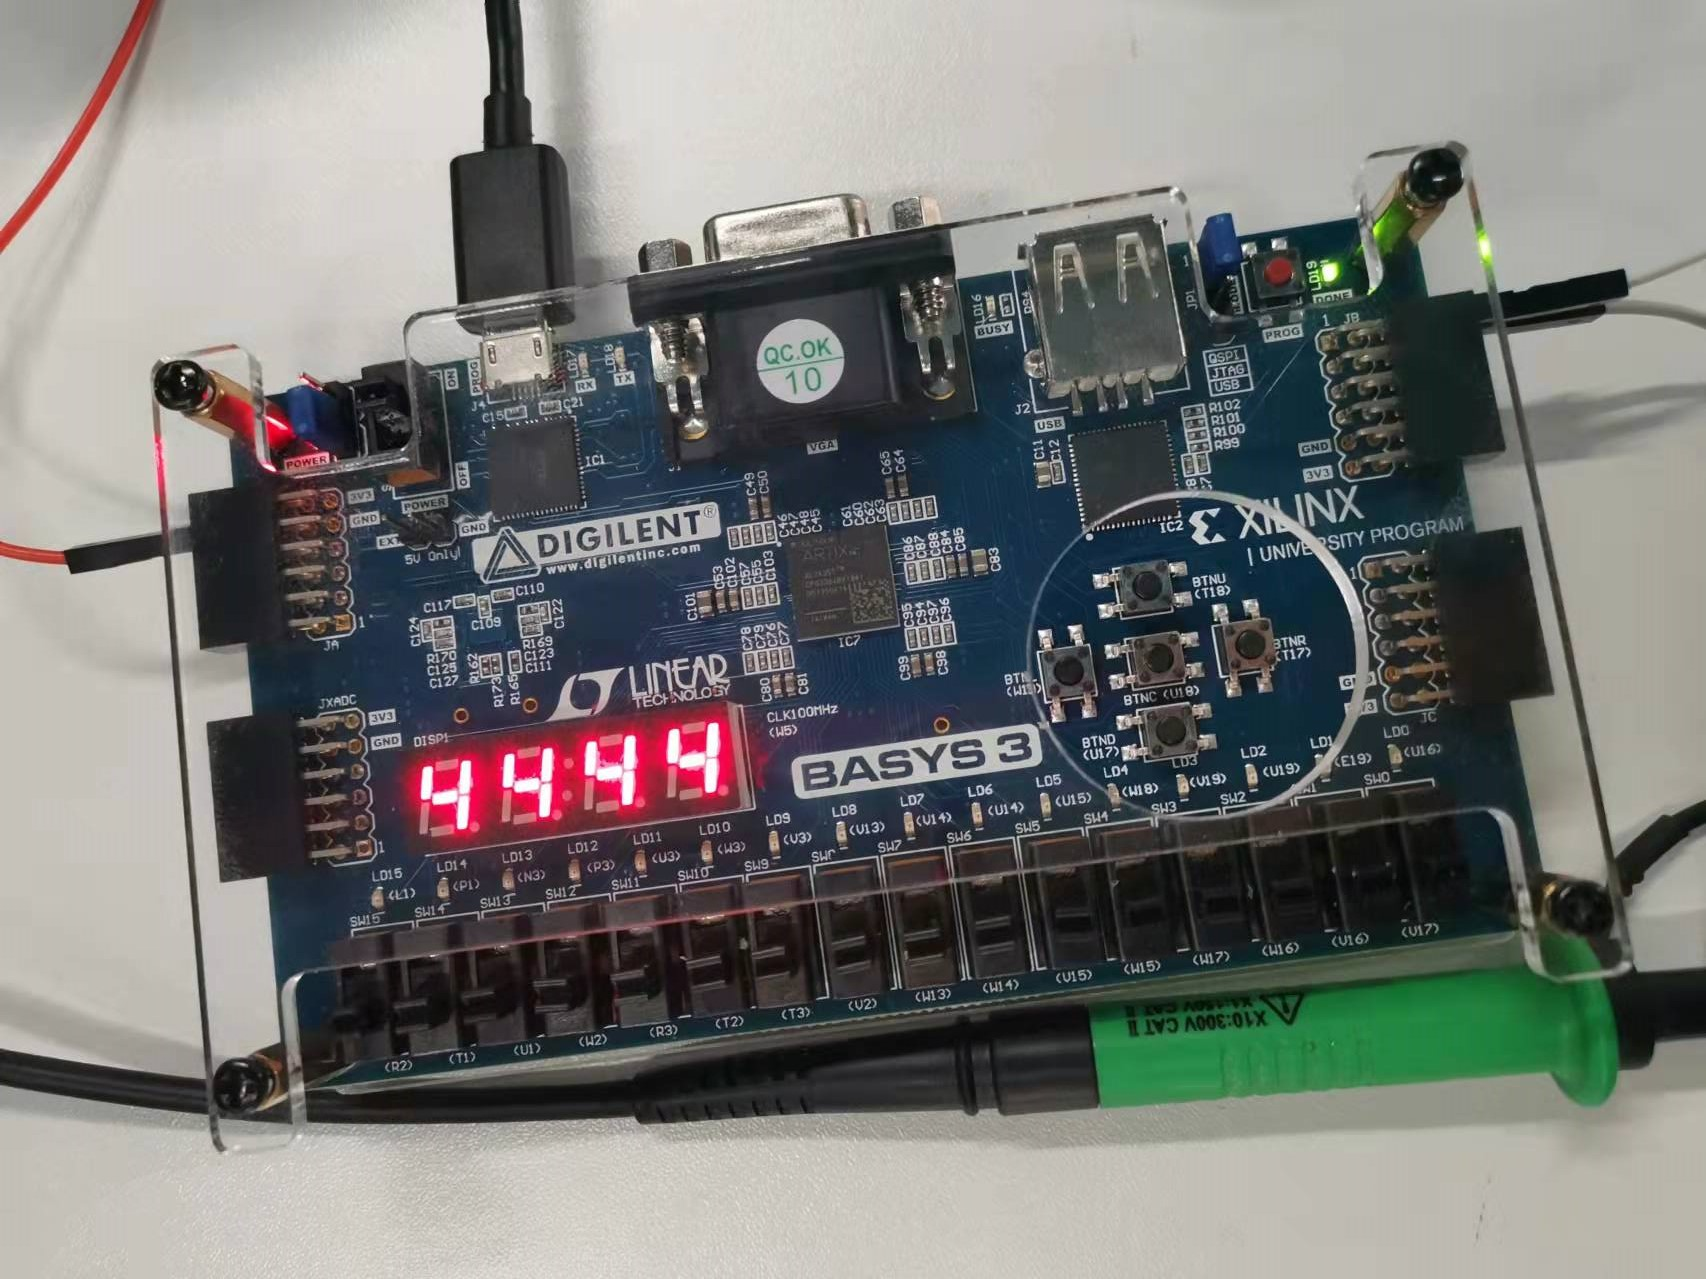
\includegraphics[width=0.22\textwidth]{original pic/4.jpg}}
    \subfigure[5]{
    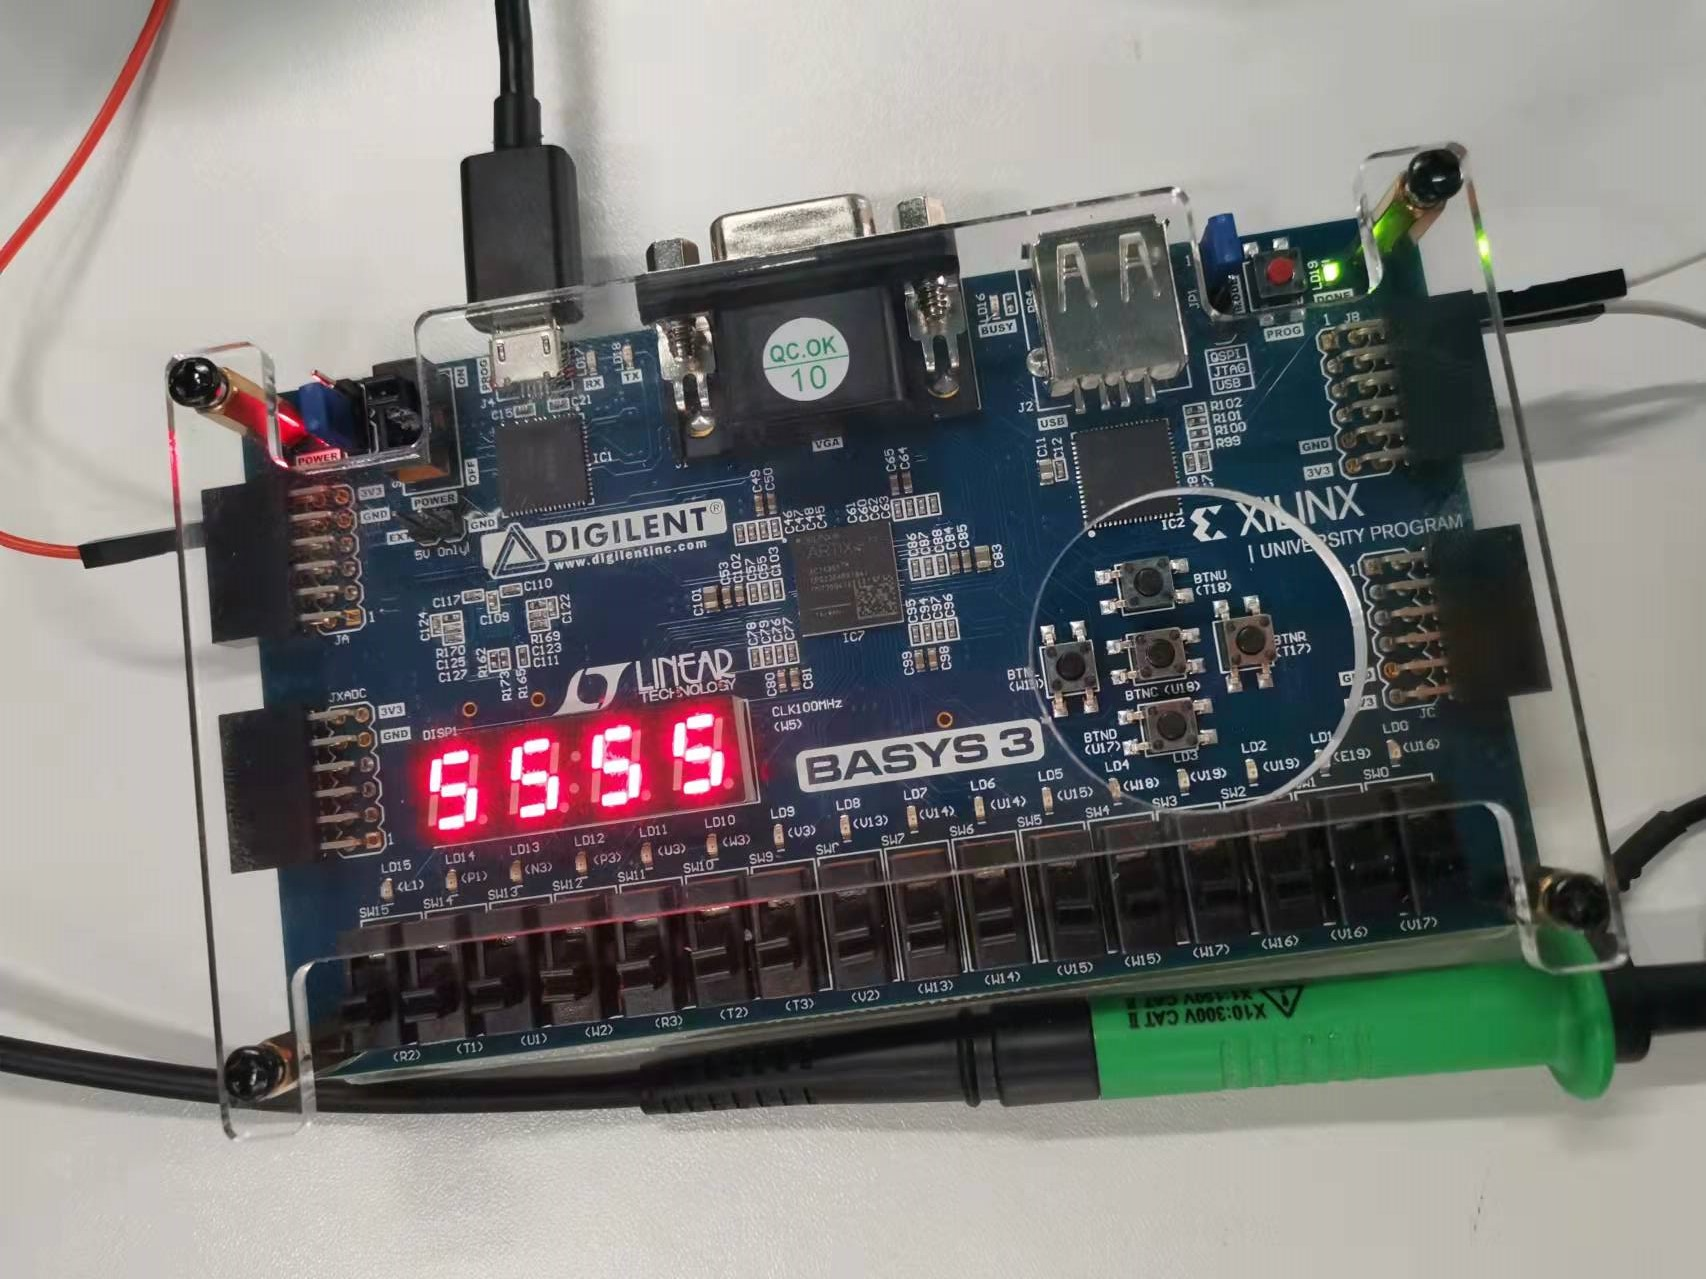
\includegraphics[width=0.22\textwidth]{original pic/5.jpg}}
    \subfigure[6]{
    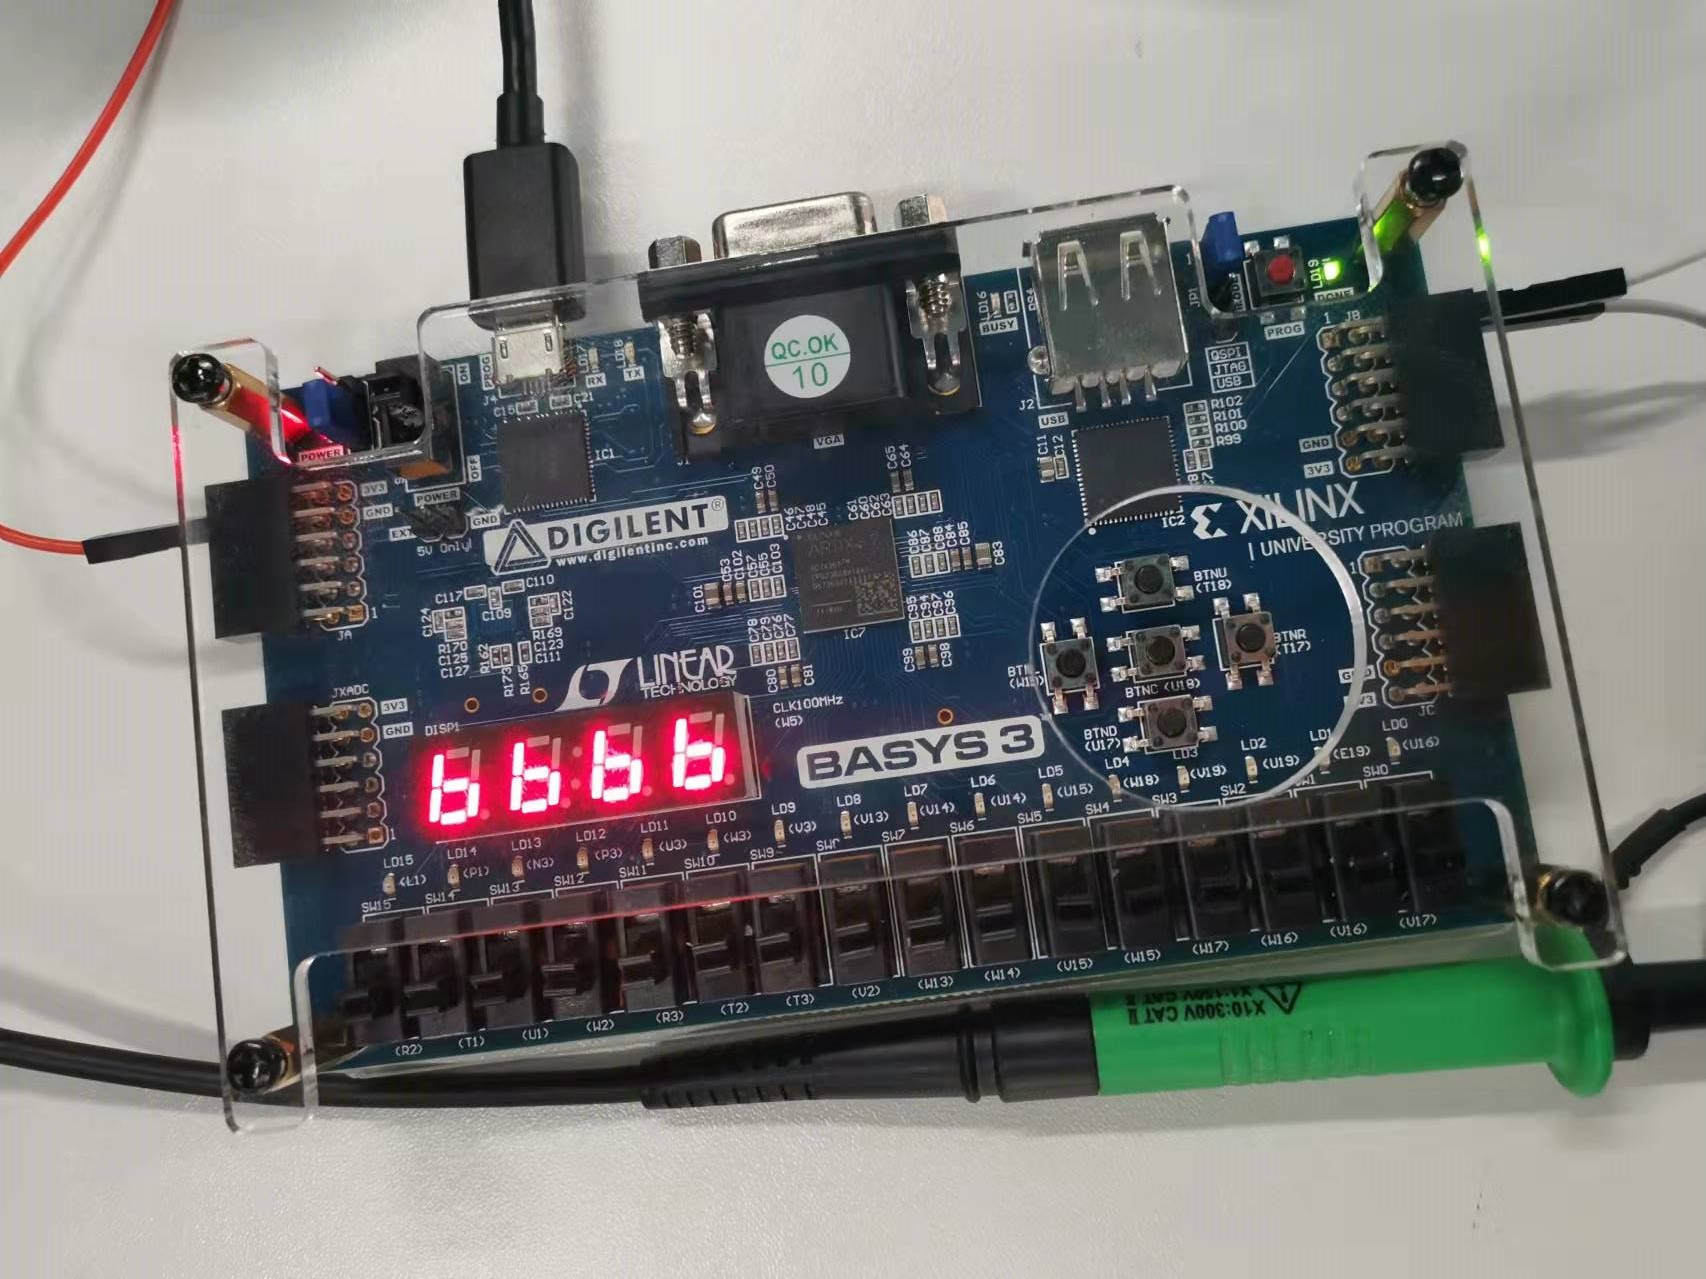
\includegraphics[width=0.22\textwidth]{original pic/6.jpg}}
    \subfigure[7]{
    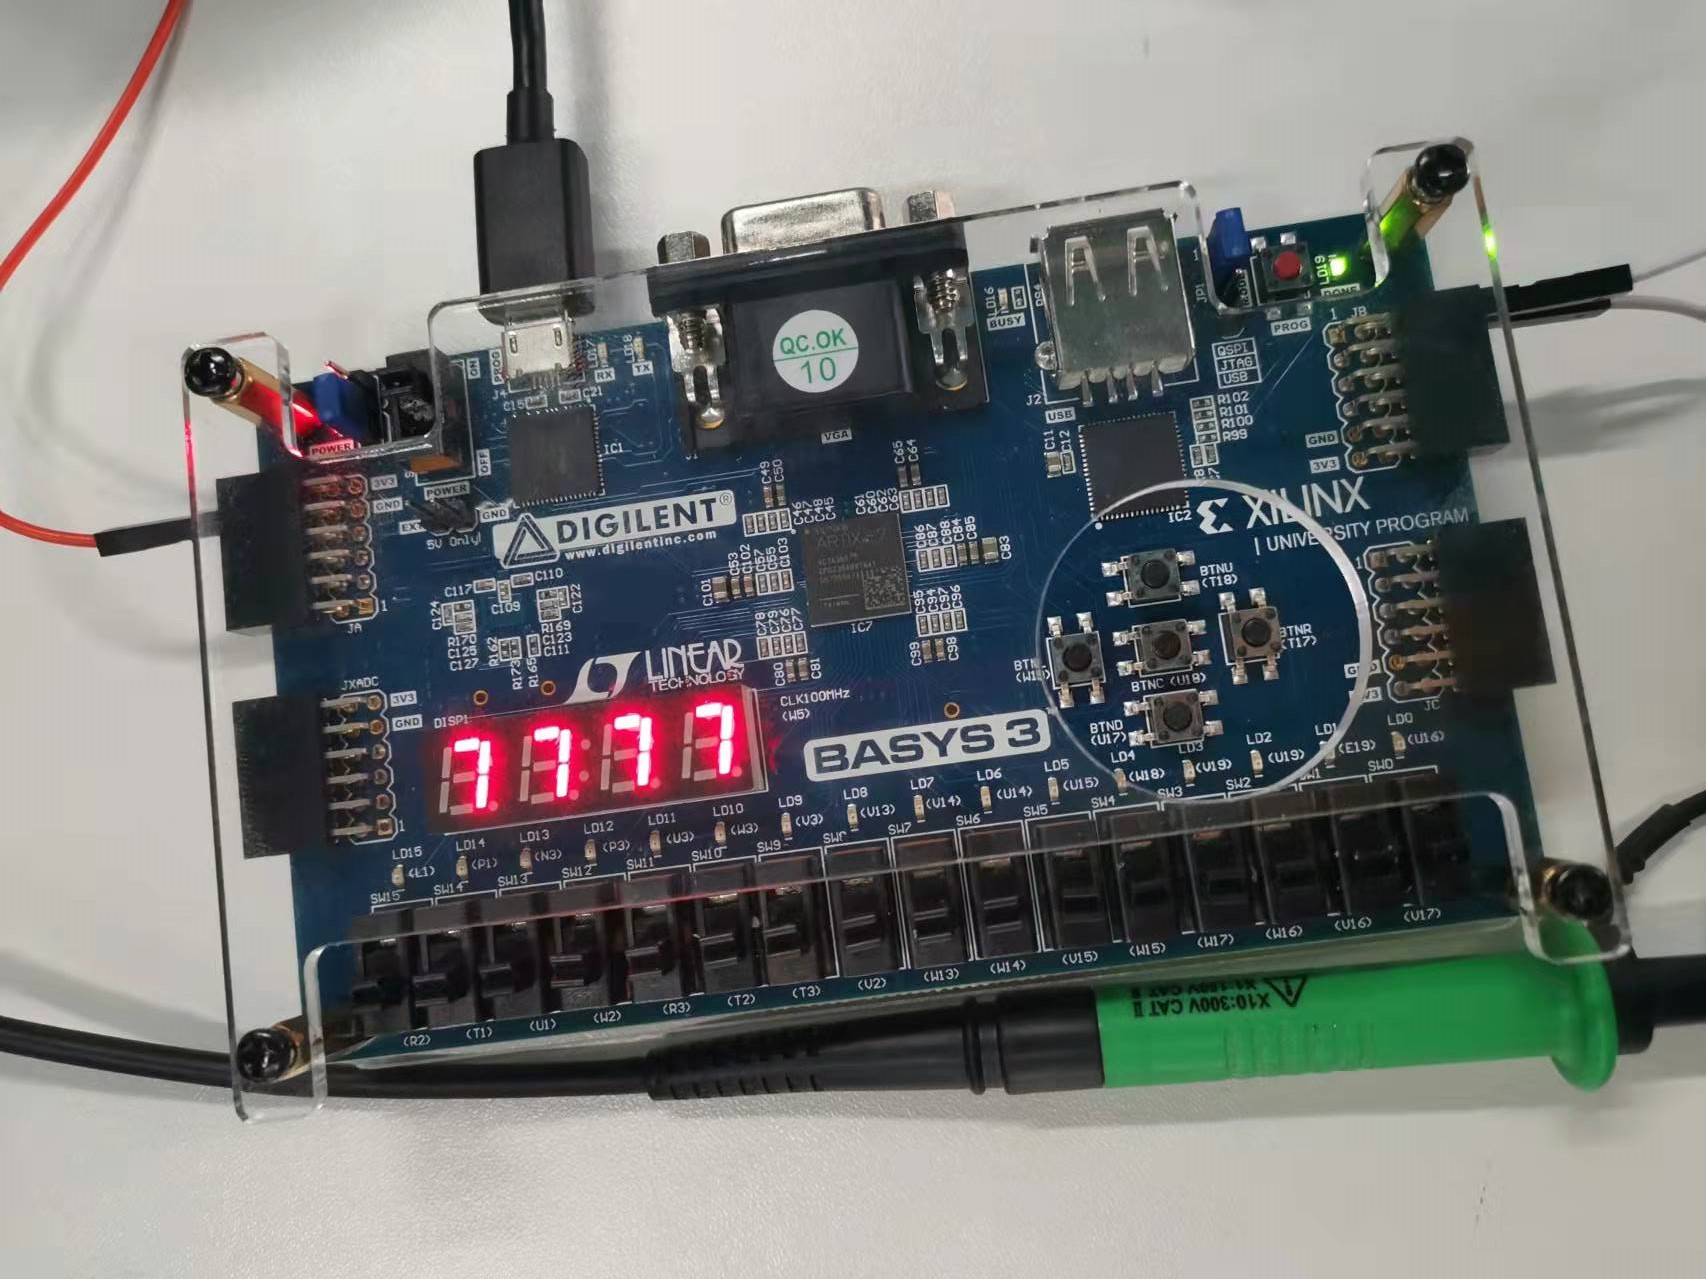
\includegraphics[width=0.22\textwidth]{original pic/7.jpg}}
    \subfigure[8]{
    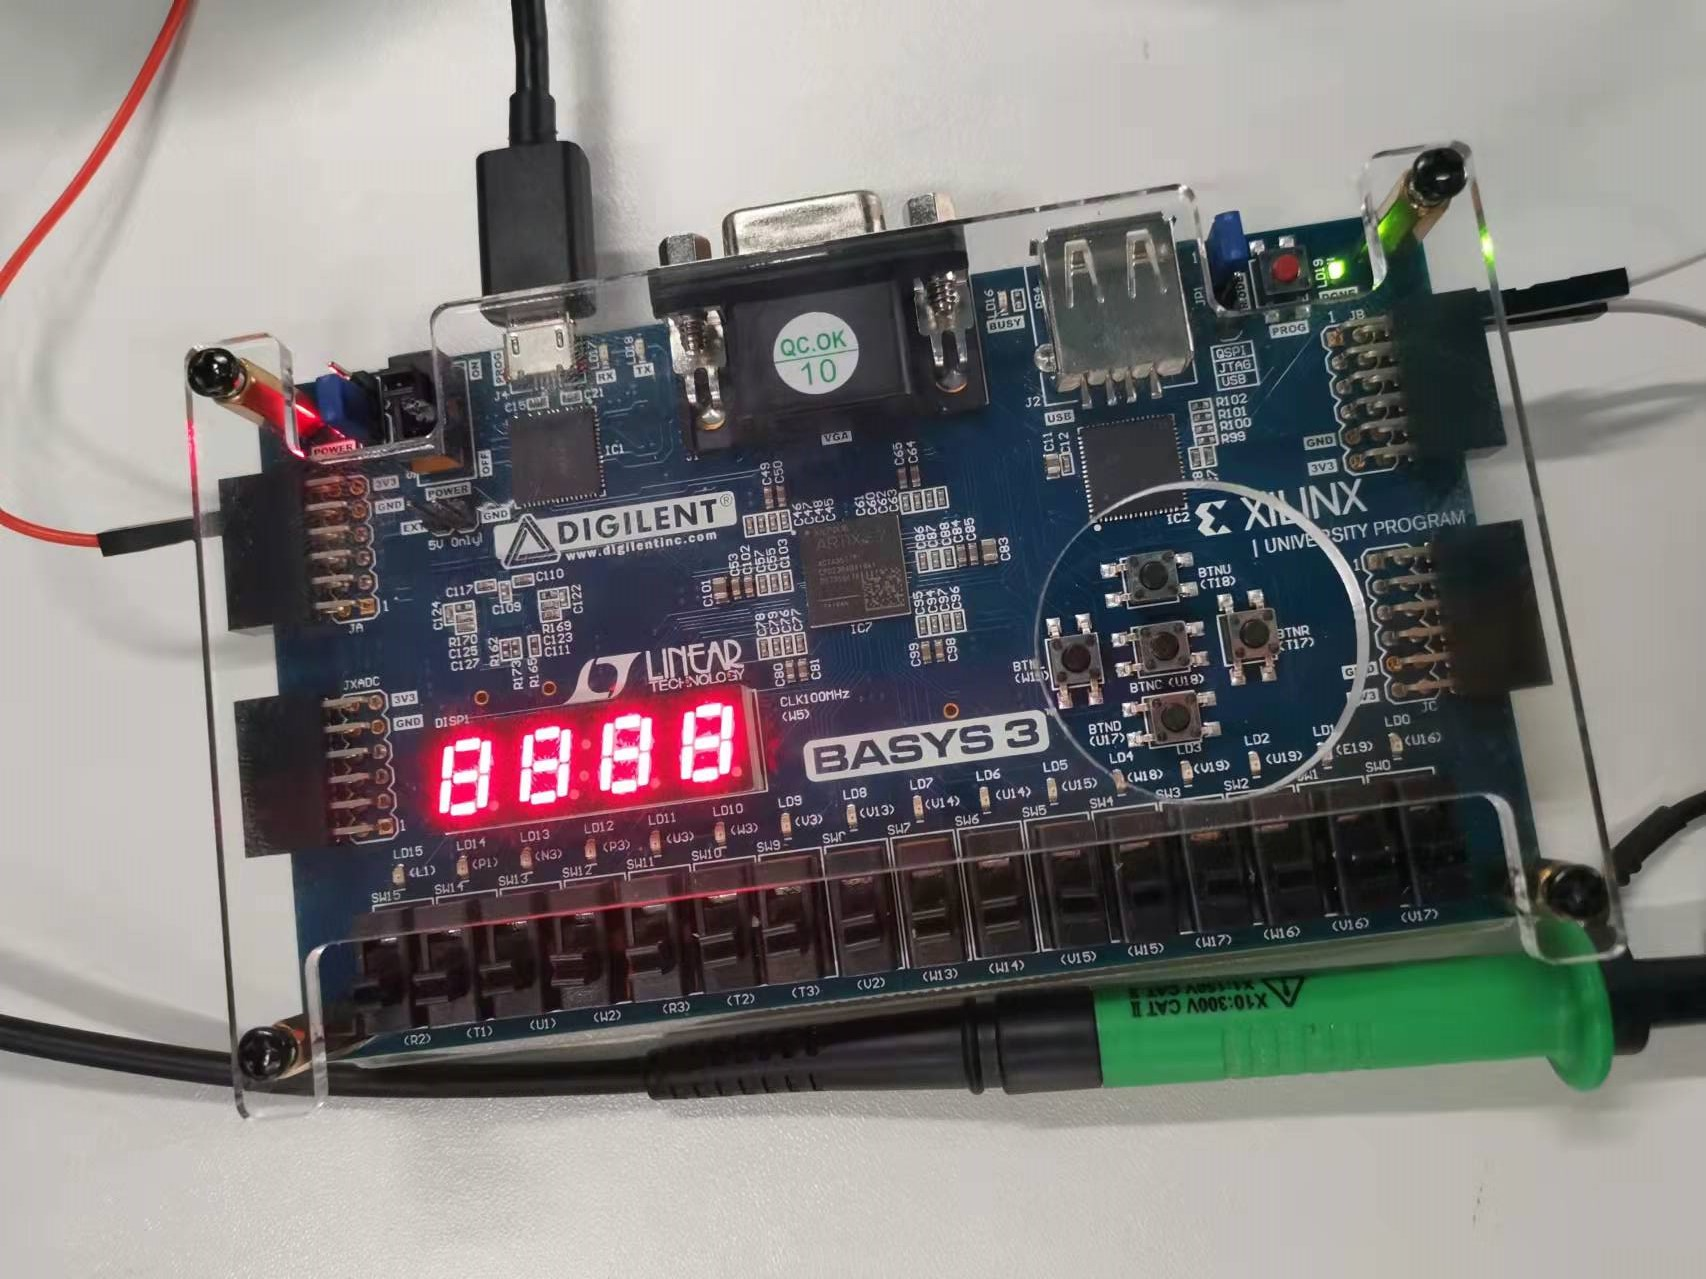
\includegraphics[width=0.22\textwidth]{original pic/8.jpg}}
    \subfigure[9]{
    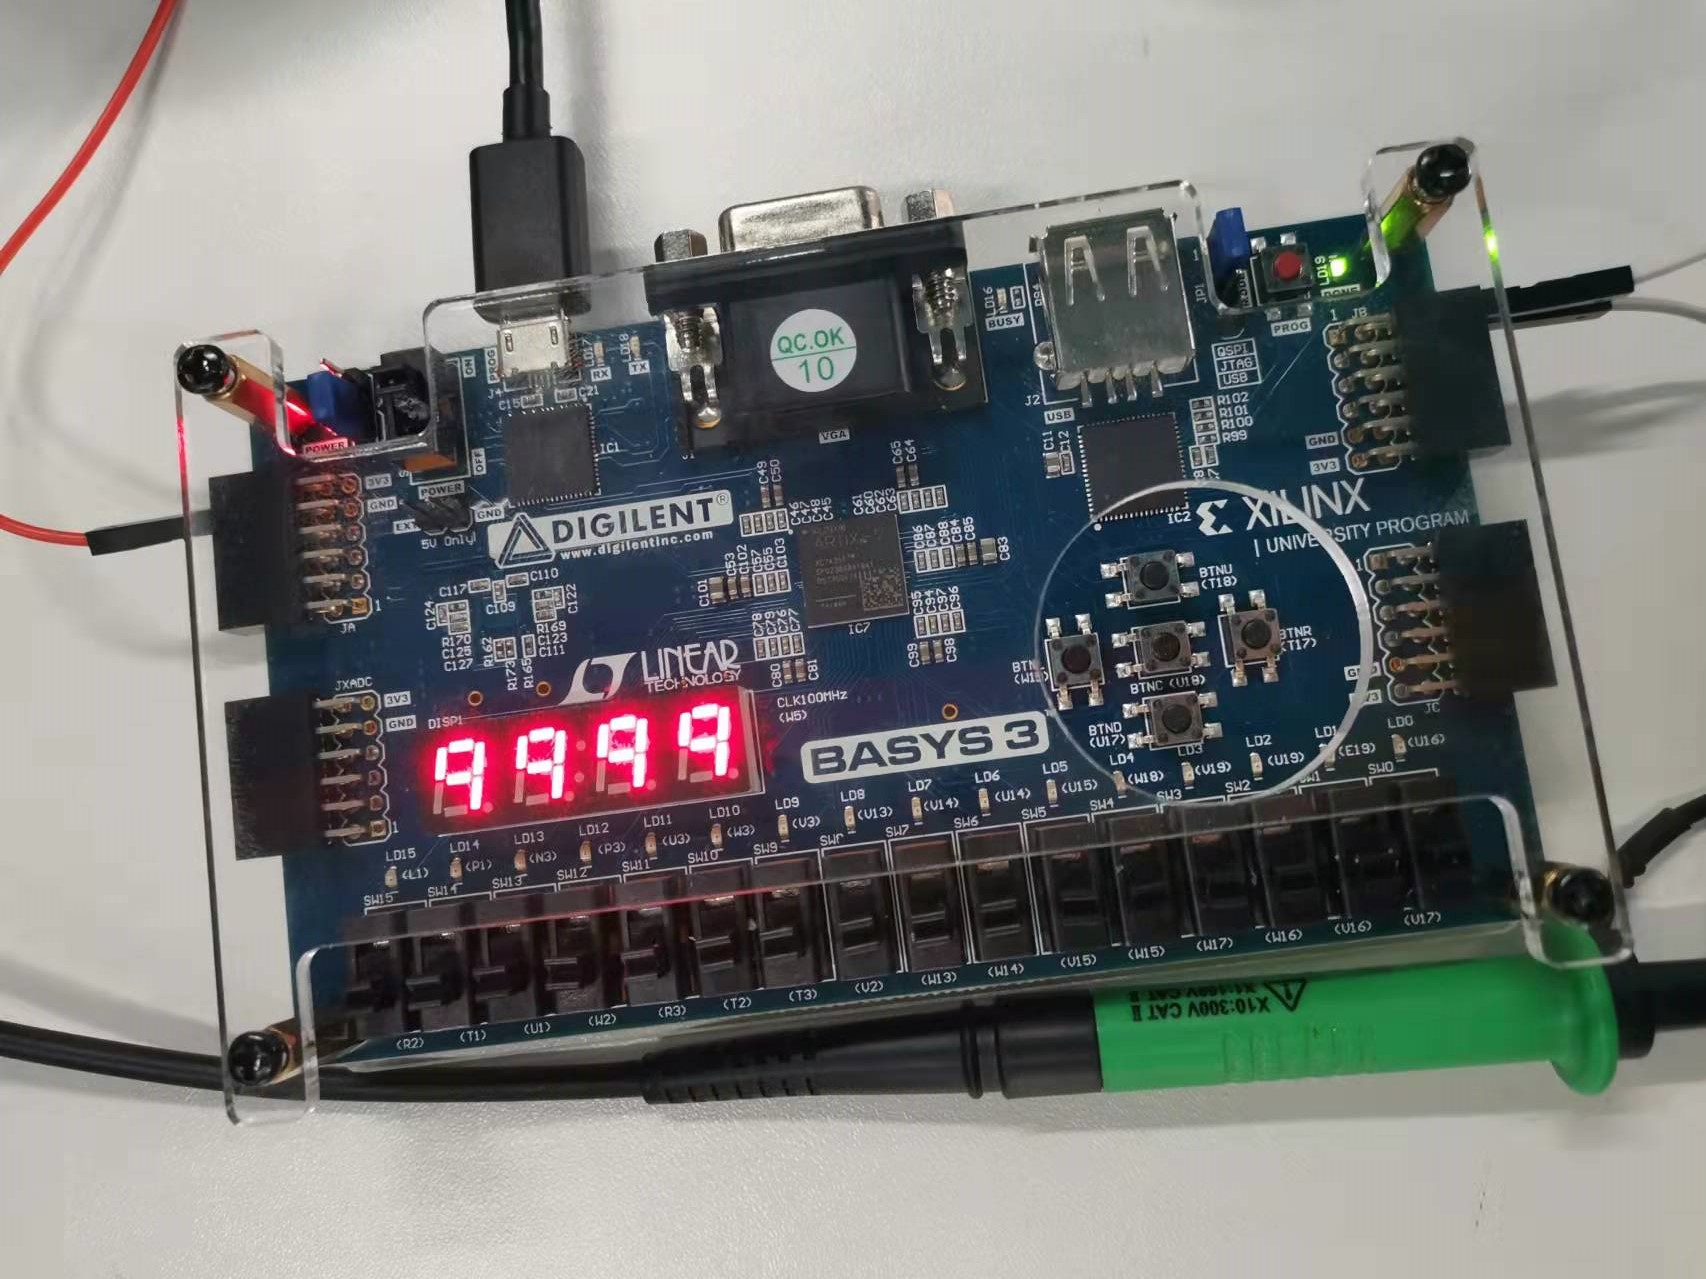
\includegraphics[width=0.22\textwidth]{original pic/9.jpg}}
    \subfigure[10]{
    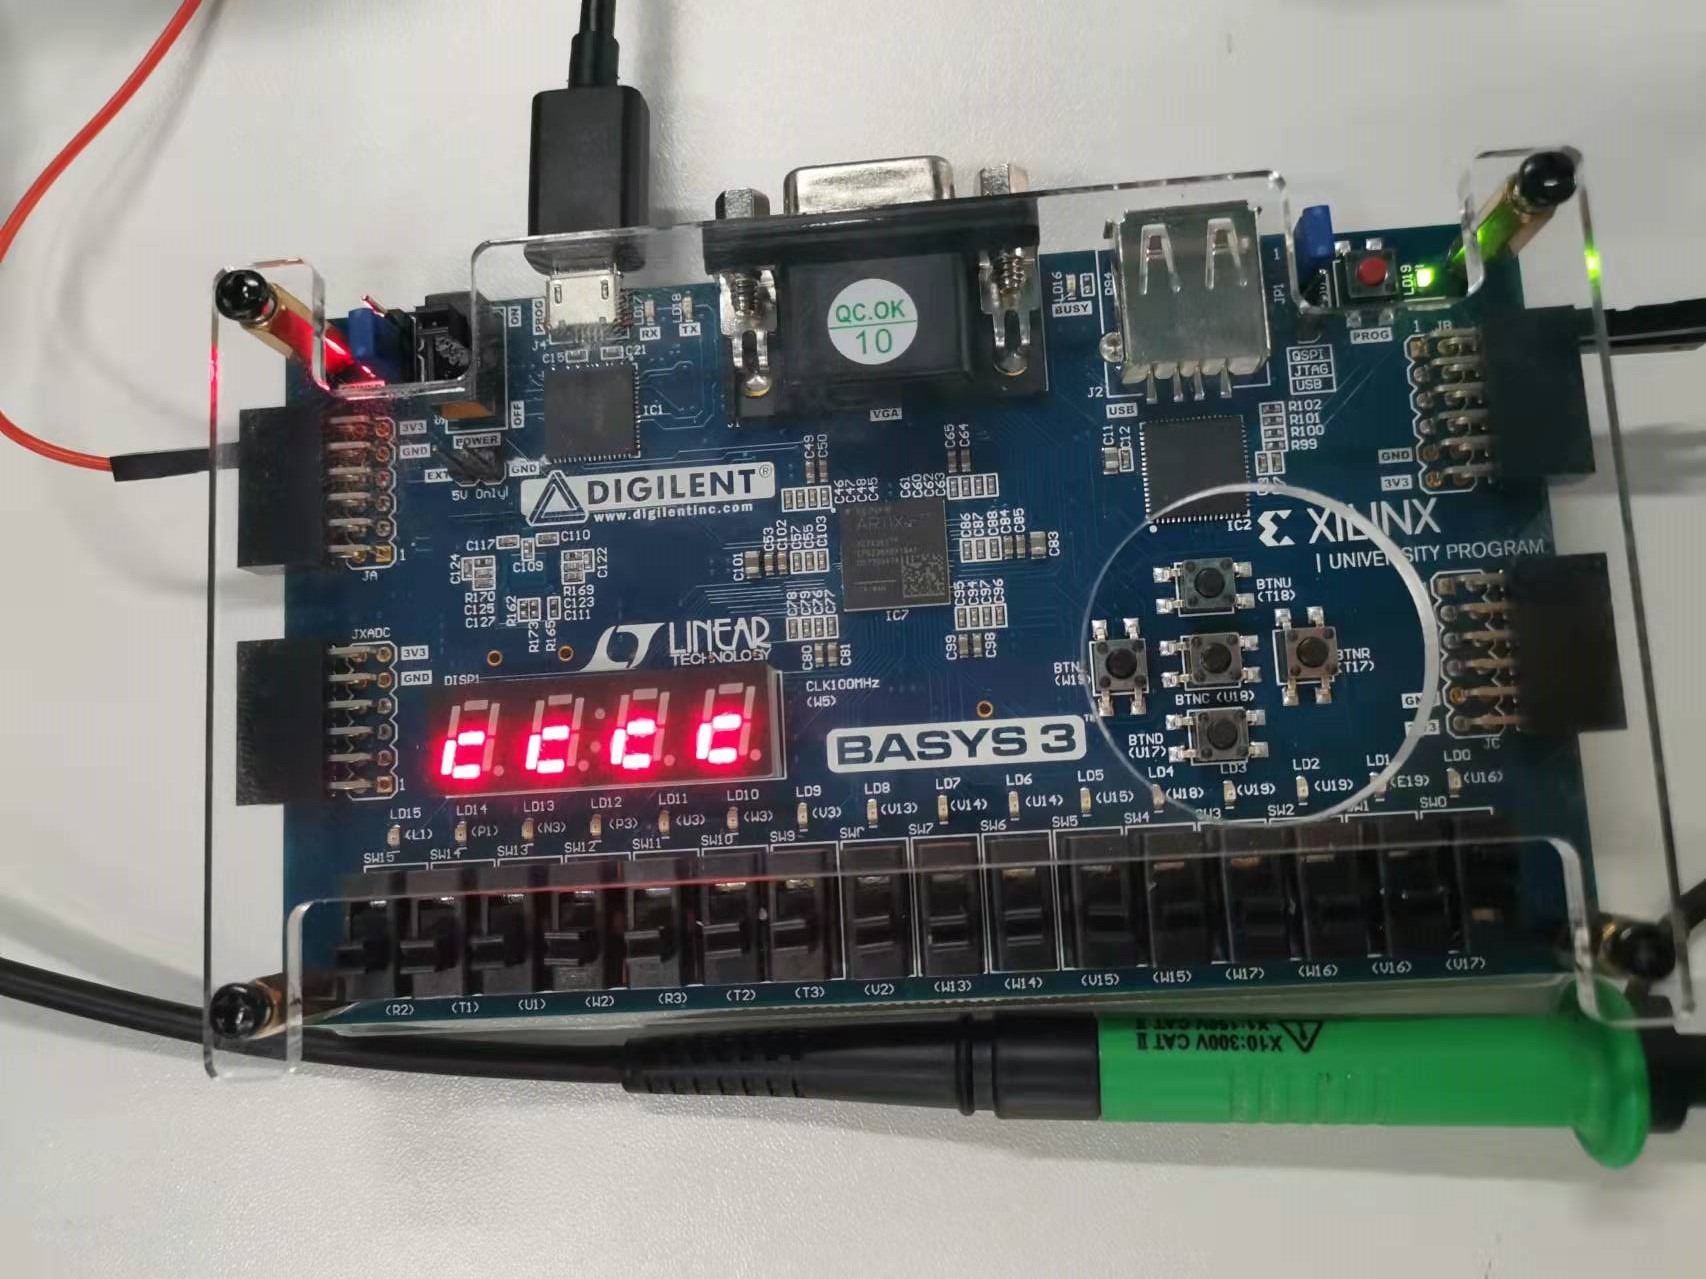
\includegraphics[width=0.22\textwidth]{original pic/10.jpg}}
    \subfigure[11]{
    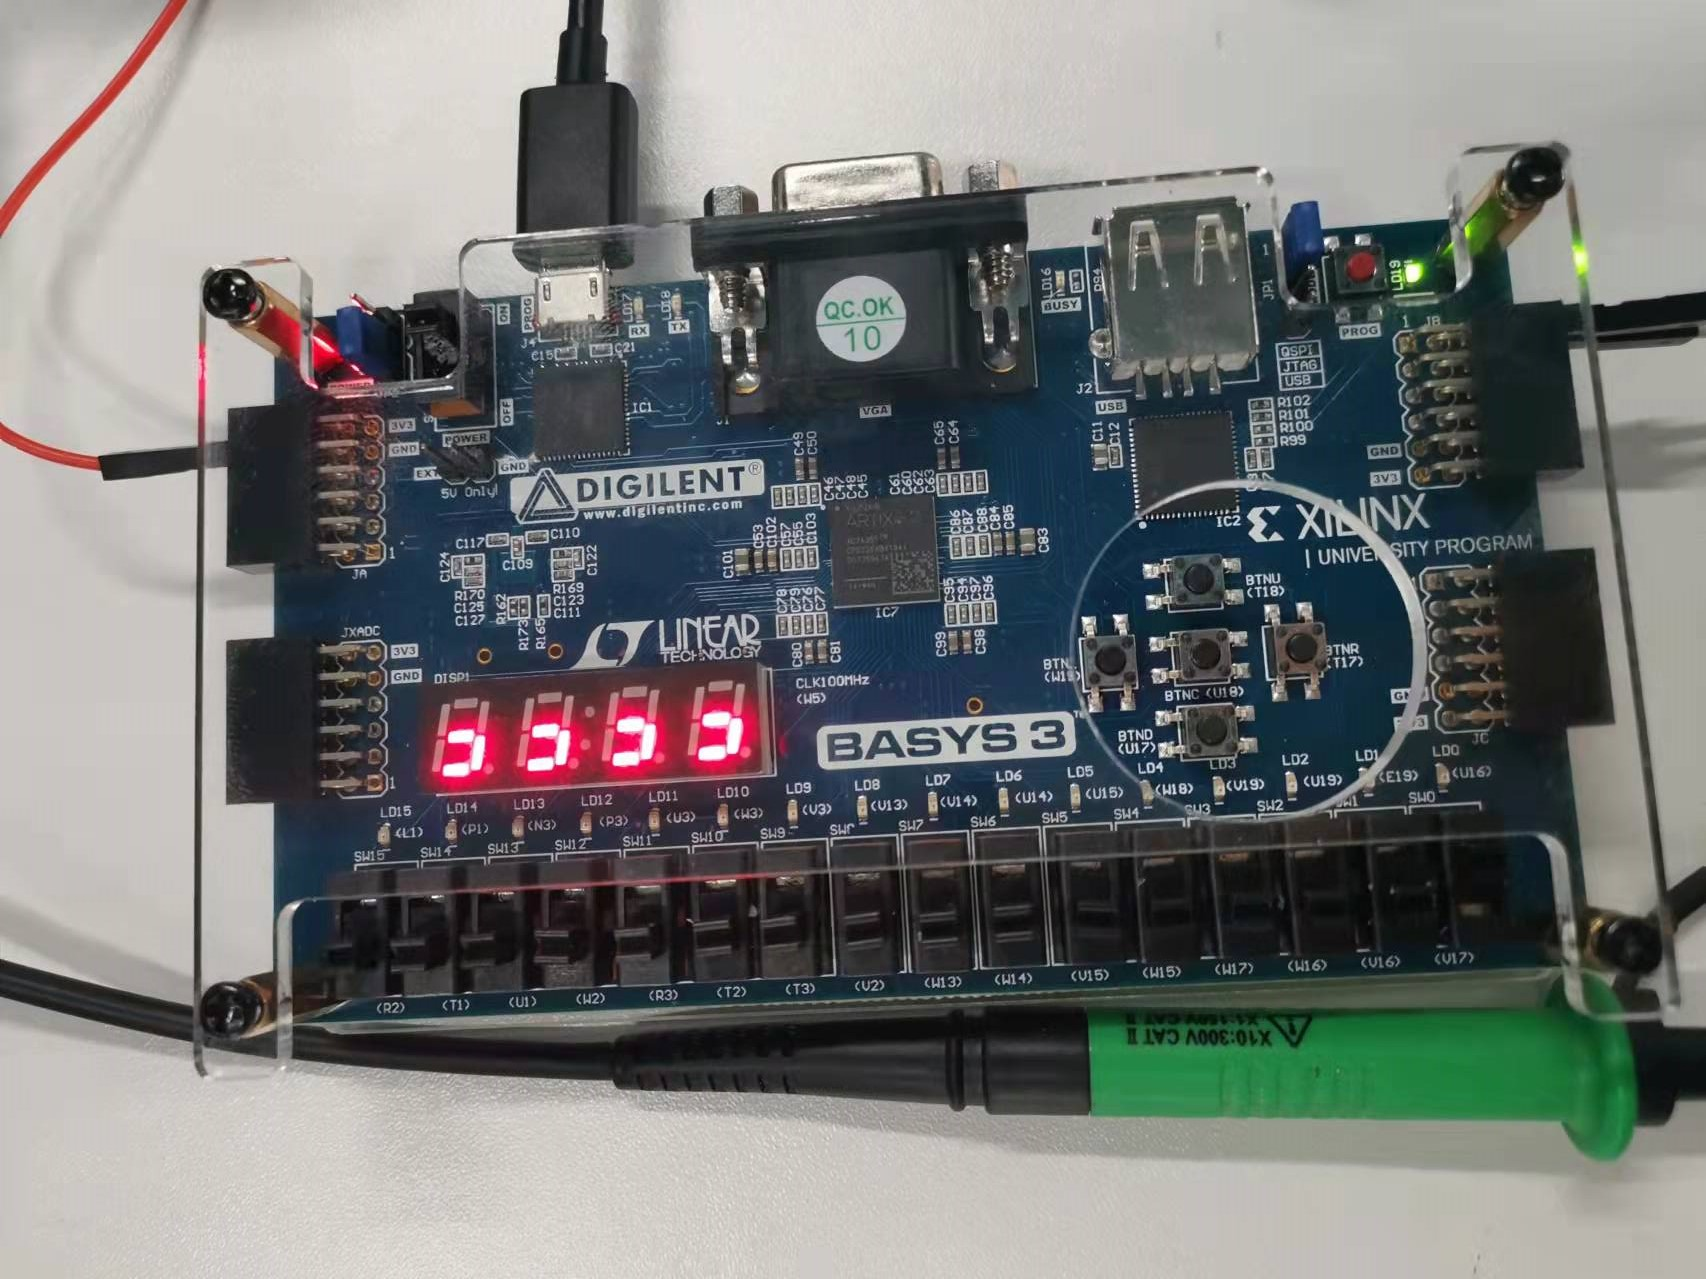
\includegraphics[width=0.22\textwidth]{original pic/11.jpg}}
    \subfigure[12]{
    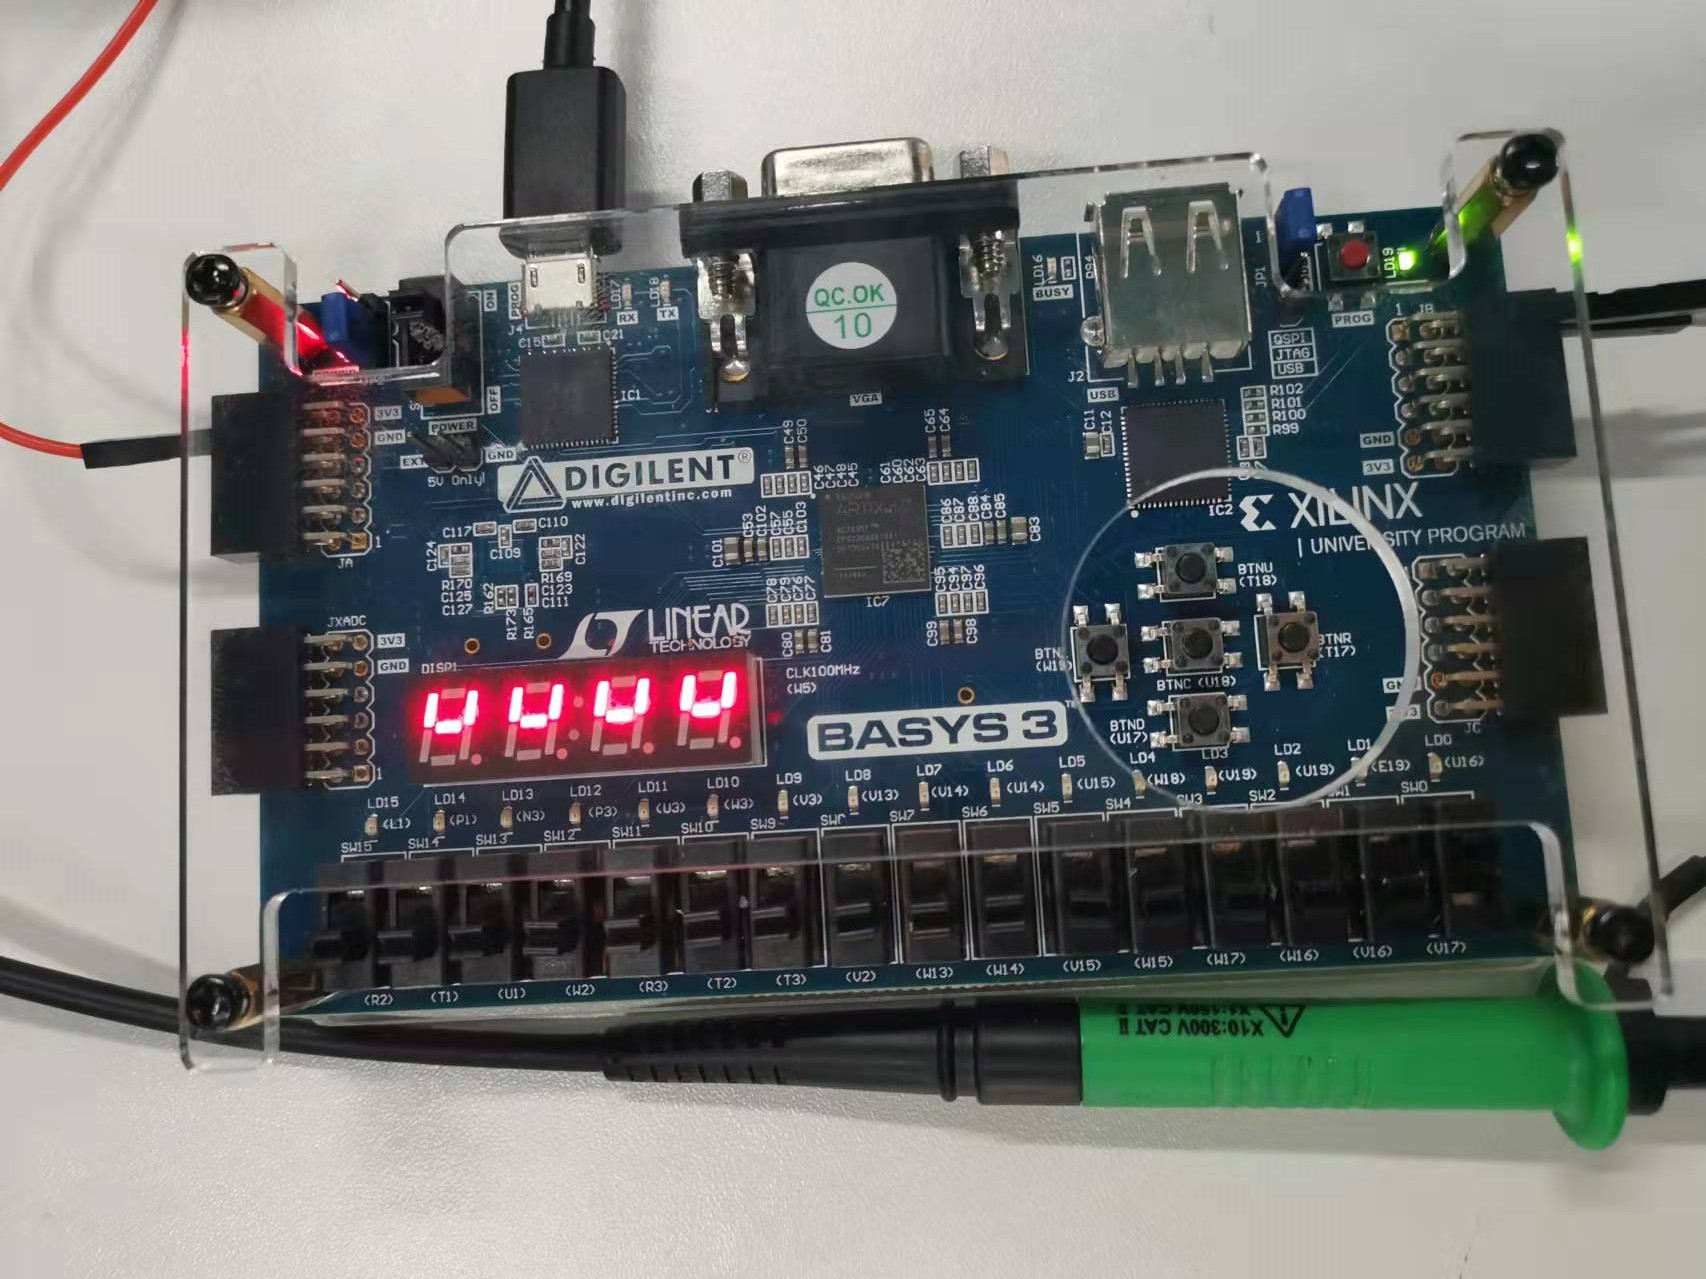
\includegraphics[width=0.22\textwidth]{original pic/12.jpg}}
    \subfigure[13]{
    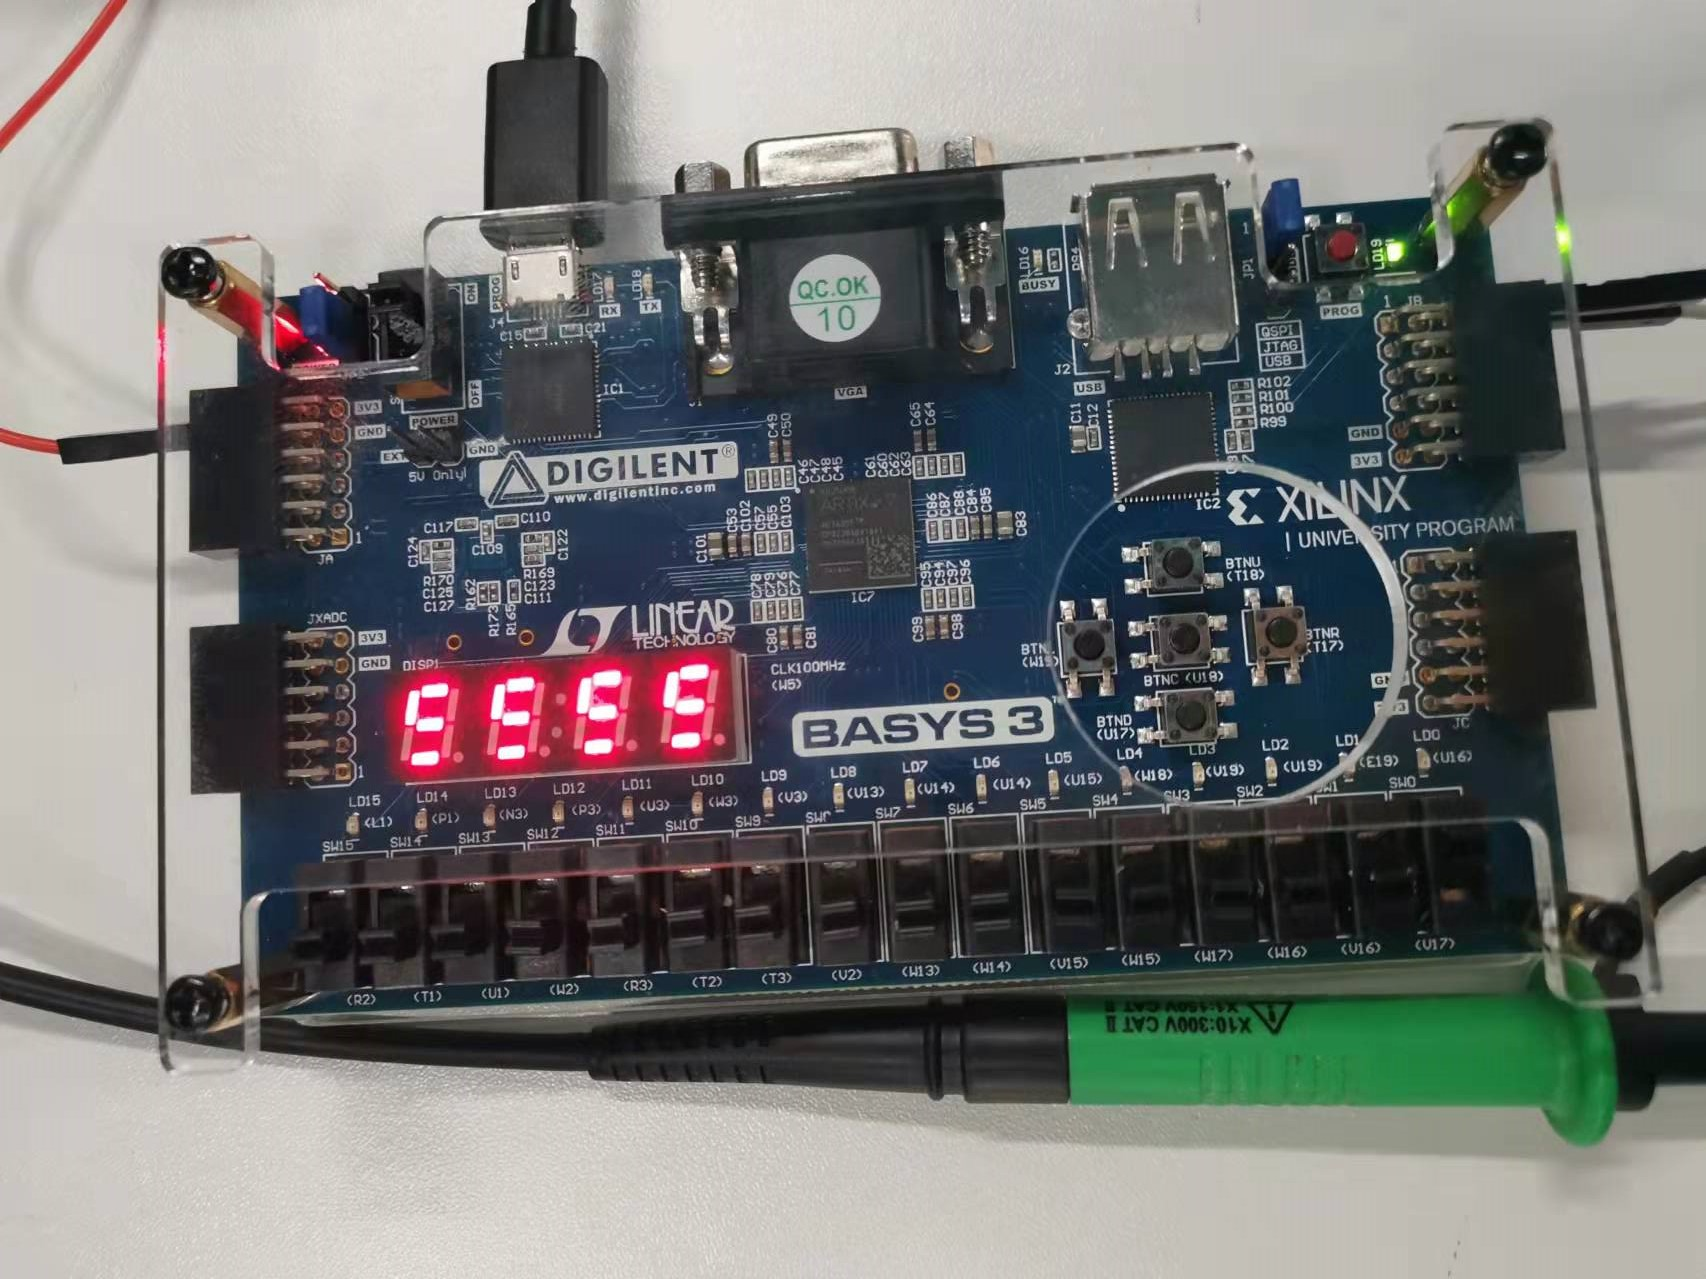
\includegraphics[width=0.22\textwidth]{original pic/13.jpg}}
    \subfigure[14]{
    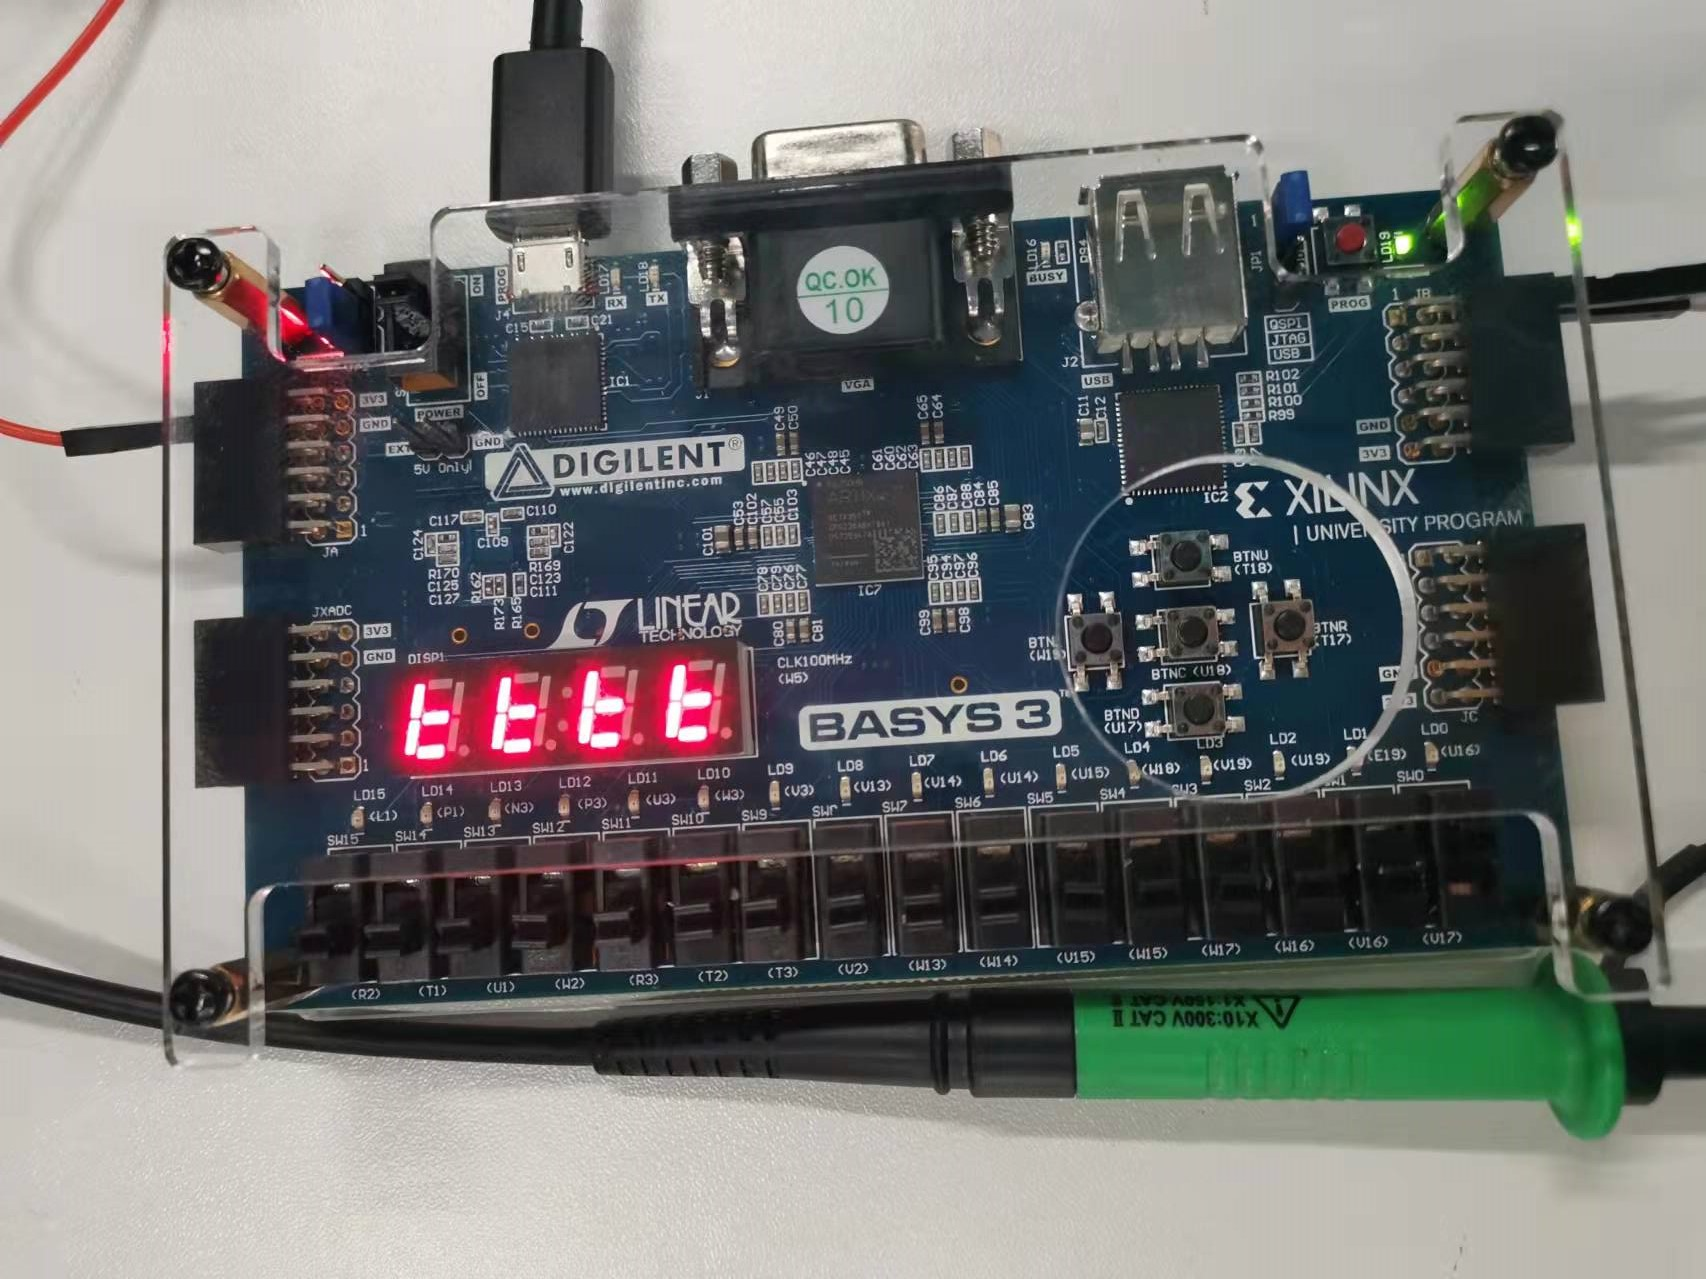
\includegraphics[width=0.22\textwidth]{original pic/14.jpg}}
    \subfigure[15]{
    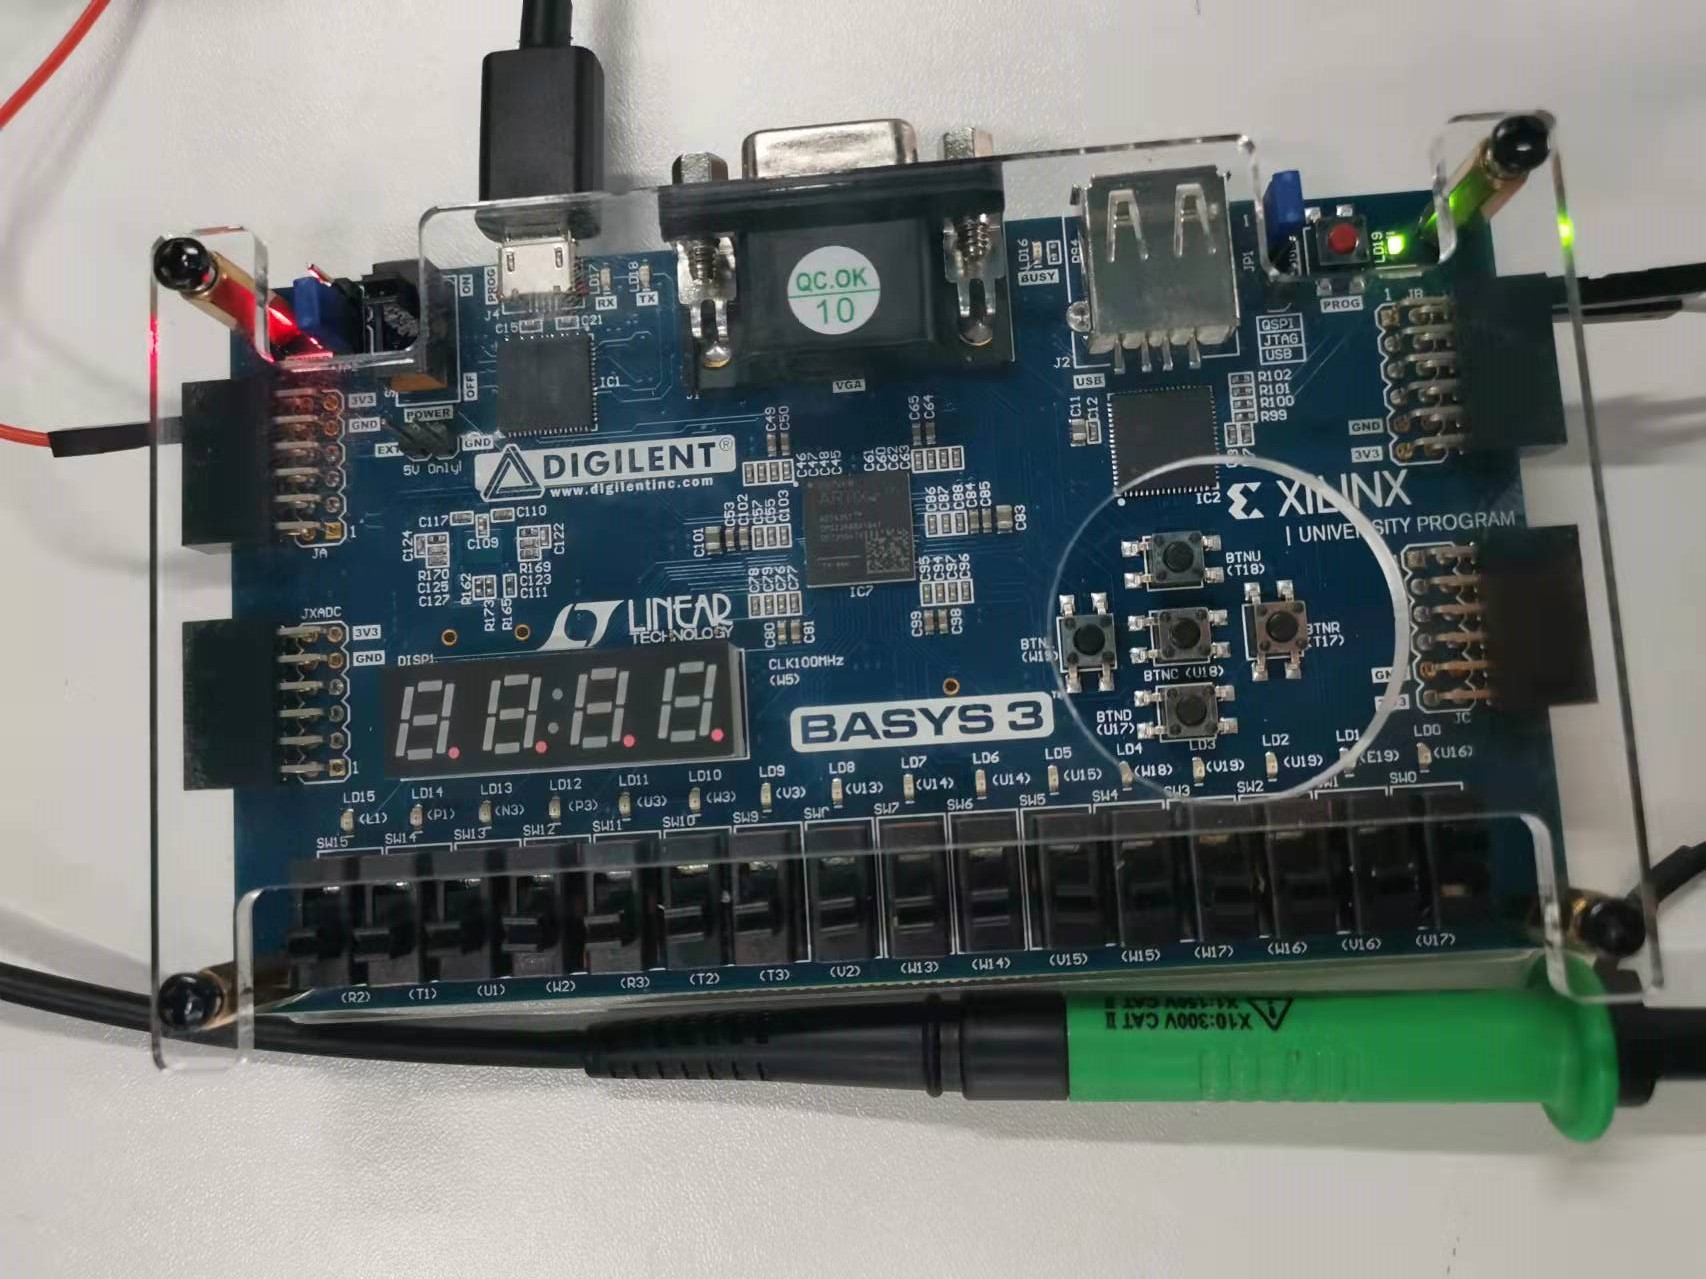
\includegraphics[width=0.22\textwidth]{original pic/15.jpg}}

    
    \caption{16进制计数器数码管显示}
    \label{16counter_slow}
\end{figure}

\(SW_0 =1 ,  SW_1 = 1\)时,时钟周期为\SI{3}{\kHz},数码管由于视觉暂留现象全亮,此时使用示波器观察计数器各输出引脚波形如图\ref{16counter_fast}所示。可以看出,在计数器一个全周期内共经历了16个时钟周期,与16进制计数器要求相符。

\begin{figure}[H]
    \centering
    \subfigure[\(JB_1\)]{
    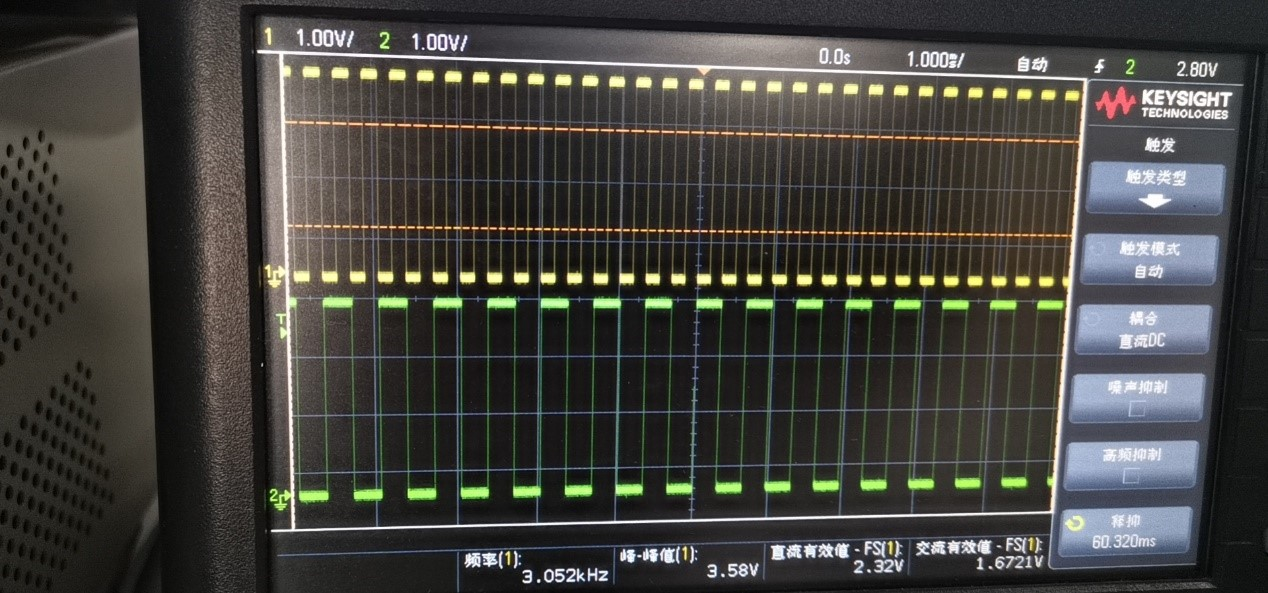
\includegraphics[width=0.45\textwidth]{16/jb1.jpg}}
    \subfigure[\(JB_2\)]{
    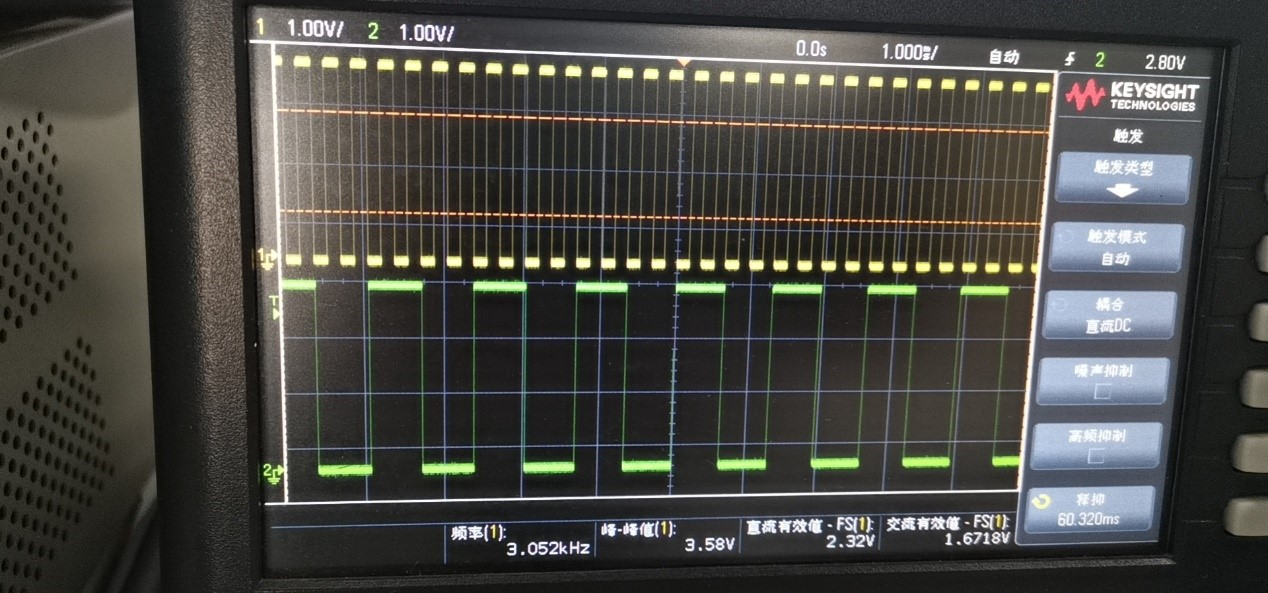
\includegraphics[width=0.45\textwidth]{16/jb2.jpg}}
    \subfigure[\(JB_3\)]{
    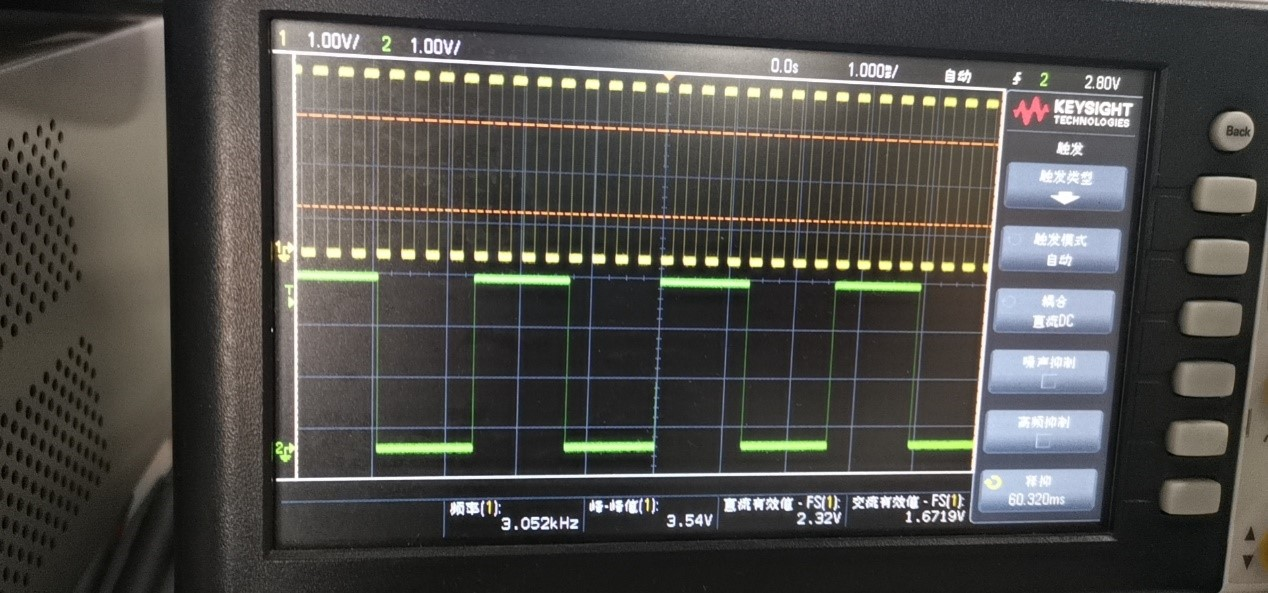
\includegraphics[width=0.45\textwidth]{16/jb3.jpg}}
    \subfigure[\(JB_4\)]{
    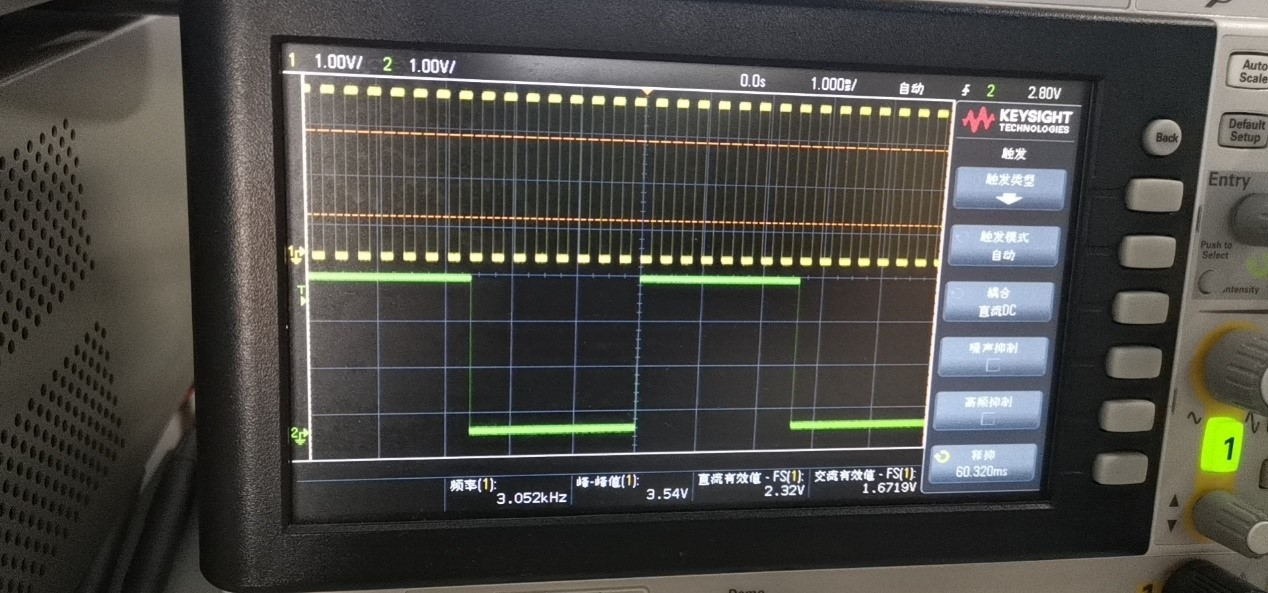
\includegraphics[width=0.45\textwidth]{16/jb4.jpg}}

    
    \caption{16进制计数器引脚输出波形}
    \label{16counter_fast}
\end{figure}

\subsubsection{小结}
\begin{itemize}
    \item 观察了16进制计数器连接数码管可以实现16种数码循环显示的功能。
    \item 测量了16进制计数器的输出波形,符合16个时钟周期1循环的要求。
\end{itemize}

\subsection{六进制计数器(置零法)}

\subsubsection{实验步骤}
\par 利用计数器的置零端,使得计数器输出为二进制6,即“0110”时,计数器置零端全部为高电平,将计数器输出置零,使得计数器仅有数字0到数字5共6个稳态,成为六进制计数器。
\par 改变置零端连接后的电路图如图\ref{6set0 circuit}所示。
\par 生成bit文件,下载到开发板上,观察实验现象。

\begin{figure}[H]
    \begin{center}
        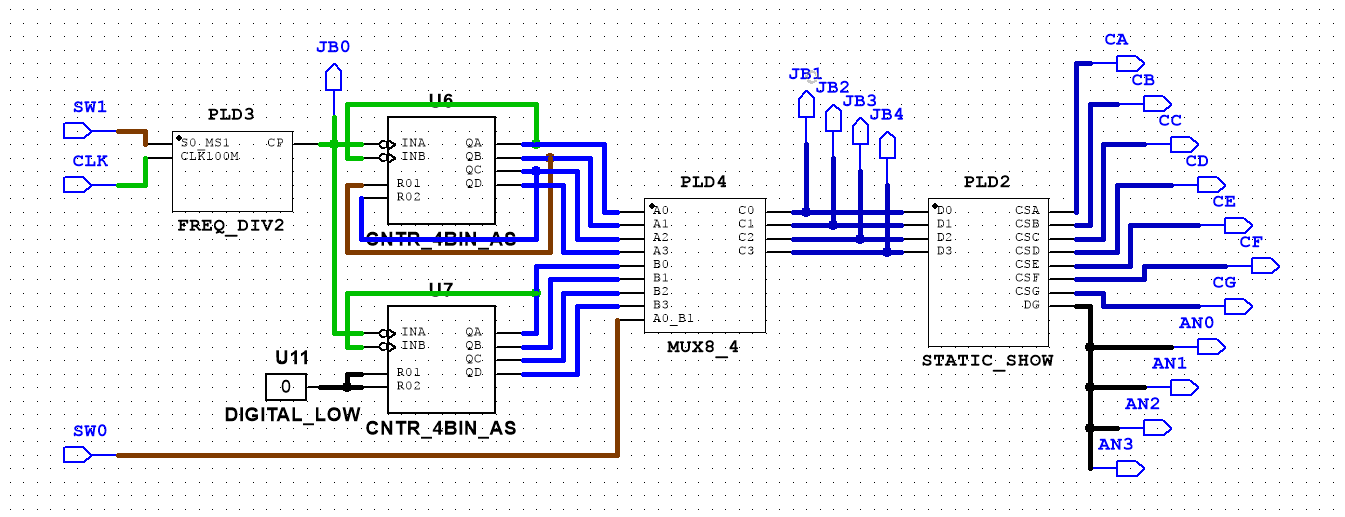
\includegraphics[width=0.8\textwidth]{6set0/ciruit.png}
    \end{center}
    \caption{六进制计数器(置零法)电路图}
    \label{6set0 circuit}
\end{figure}


\subsubsection{实验结果}
\(SW_0 = SW_1 = 0\)时,时钟周期为\SI{0.75}{\Hz},计数器数字缓慢变化。观察到十进制计数器共有6个稳态,分别显示数字\(0\sim5\),实验现象已录制成为视频“6进制计数器(置零法).mp4”,附在邮件中。

\par \(SW_0 =0 ,  SW_1 = 1\)时,时钟周期为\SI{3}{\kHz},数码管由于视觉暂留现象全亮,此时使用示波器观察计数器各输出引脚波形如图\ref{6set0}所示。可以看出,在计数器一个全周期内共经历了6个时钟周期,与六进制计数器要求相符。

\begin{figure}[H]
    \centering
    \subfigure[\(JB_1\)]{
    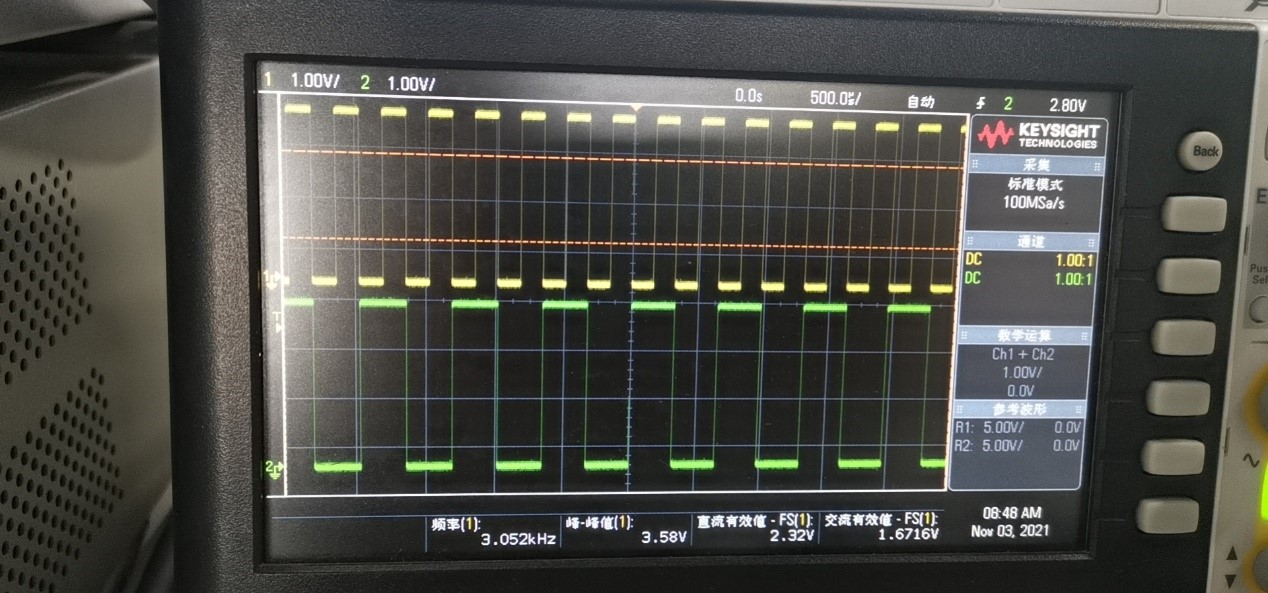
\includegraphics[width=0.45\textwidth]{6set0/jb1.jpg}}
    \subfigure[\(JB_2\)]{
    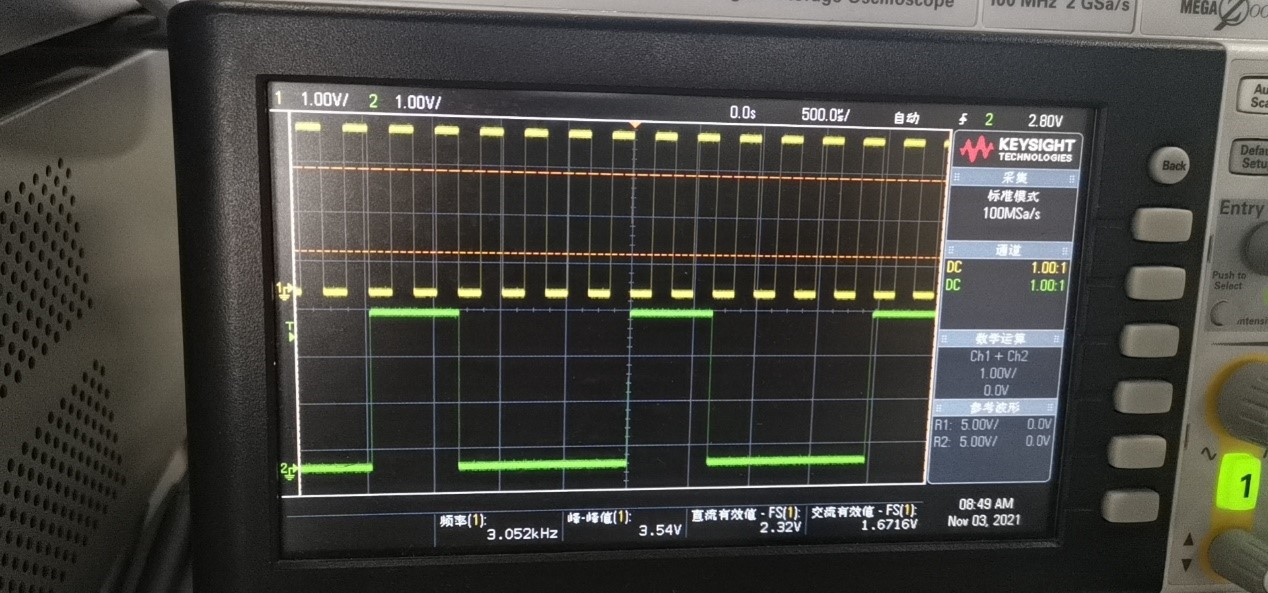
\includegraphics[width=0.45\textwidth]{6set0/jb2.jpg}}
    \subfigure[\(JB_3\)]{
    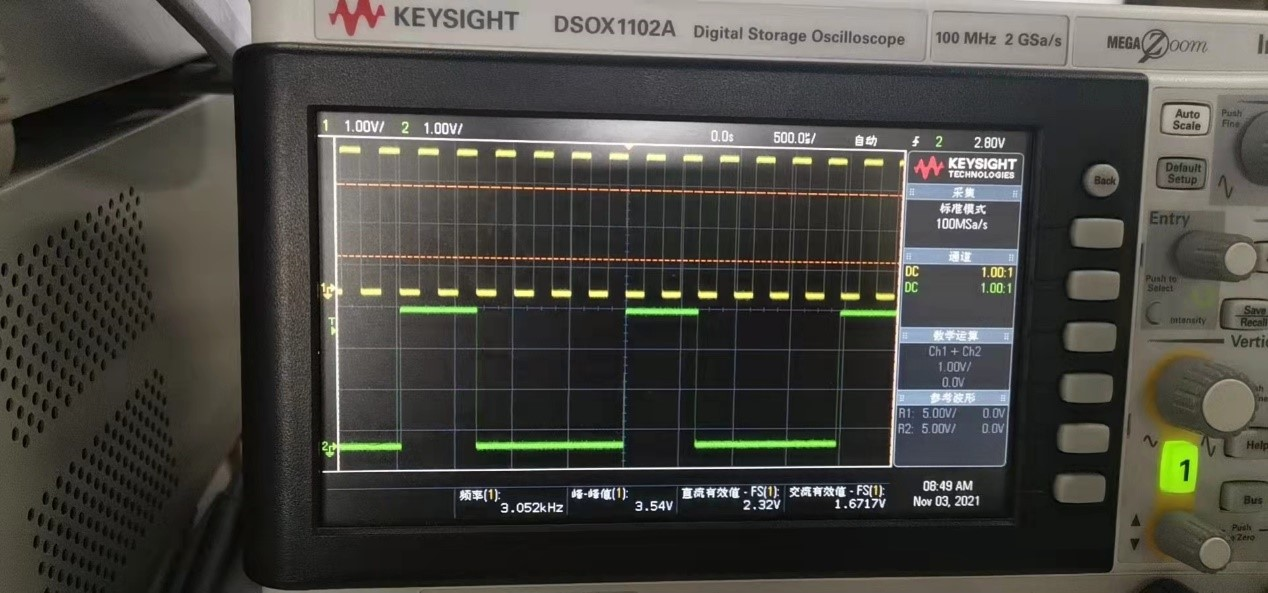
\includegraphics[width=0.45\textwidth]{6set0/jb3.jpg}}
    \subfigure[\(JB_4\)]{
    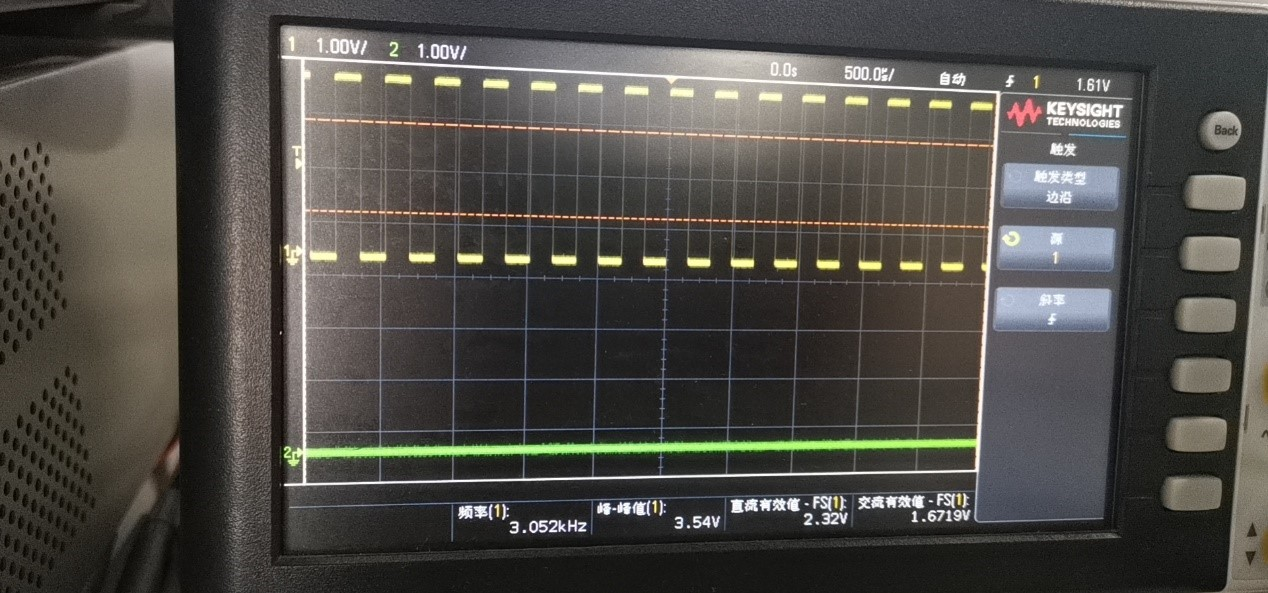
\includegraphics[width=0.45\textwidth]{6set0/jb4.jpg}}

    \caption{六进制计数器引脚输出波形}
    \label{6set0}
\end{figure}

\subsubsection{小结}
\begin{itemize}
    \item 熟悉了计数器置零端的用法,掌握了利用置零端使计数器数字归零,调整进位的方法。
    \item 利用置零法,在输出数字6的时候将数字置零,实现了六进制计数器。
\end{itemize}

\subsection{六进制计数器(置9法)}

\subsubsection{实验步骤}
\par 将原有计数器模块改为带置数端的计数器模块,将二进制数字9,即“1001”连接到计数器置数端。利用与非门,使得当且仅当输出为二进制4时置数使能端(\(\sim\)load)为低电平,当且仅当输出为二进制10时置零端为低电平。将计数器两使能端连接高电平,使计数器始终工作。更改后的电路图如图\ref{6set9 circuit}所示。
\par 生成bit文件,下载到开发板上,观察实验现象。

\begin{figure}[H]
    \begin{center}
        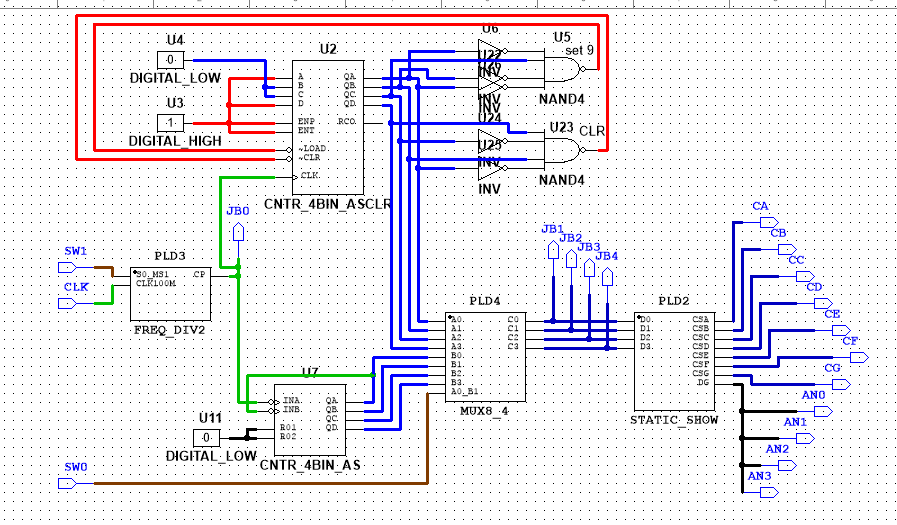
\includegraphics[width=0.8\textwidth]{6set9/circuit.png}
    \end{center}
    \caption{六进制计数器(置零法)电路图}
    \label{6set9 circuit}
\end{figure}


\subsubsection{实验结果}
\(SW_0 = SW_1 = 0\)时,时钟周期为\SI{0.75}{\Hz},计数器数字缓慢变化。观察到十进制计数器共有6个稳态,分别显示数字\(0\sim4\)以及数字9,实验现象已录制成为视频“6进制计数器(置9法).mp4”,附在邮件中。

\par \(SW_0 =0 ,  SW_1 = 1\)时,时钟周期为\SI{3}{\kHz},数码管由于视觉暂留现象全亮,此时使用示波器观察计数器各输出引脚波形如图\ref{6set9}所示。可以看出,在计数器一个全周期内共经历了6个时钟周期,与六进制计数器要求相符。

\begin{figure}[H]
    \centering
    \subfigure[\(JB_1\)]{
    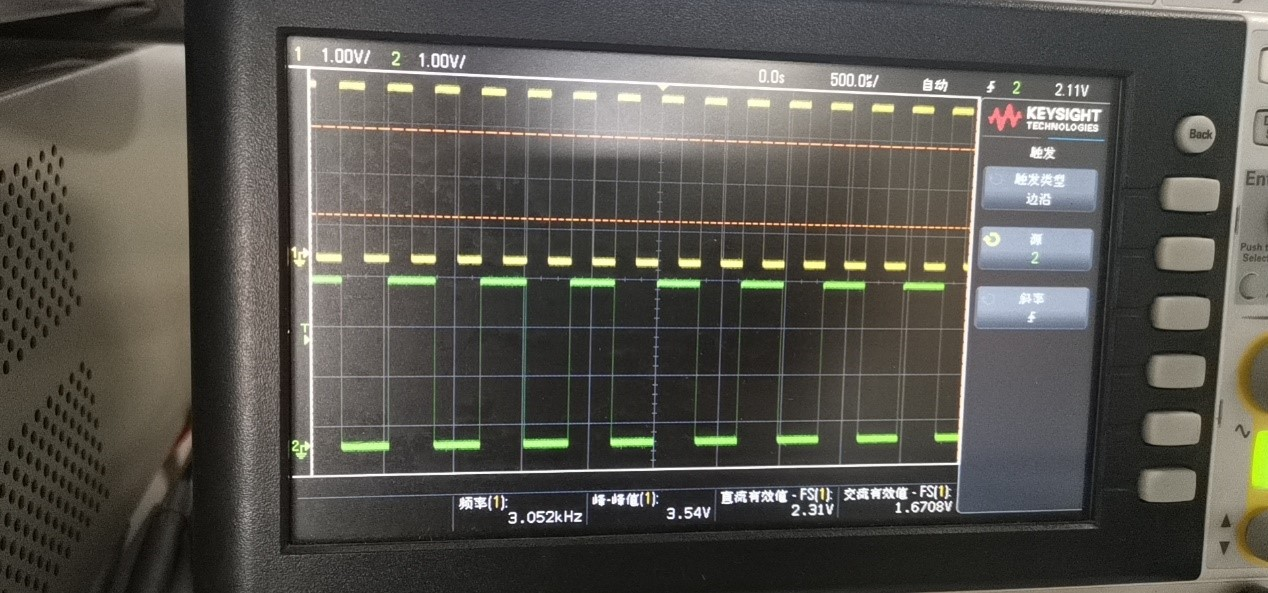
\includegraphics[width=0.45\textwidth]{6set9/jb1.jpg}}
    \subfigure[\(JB_2\)]{
    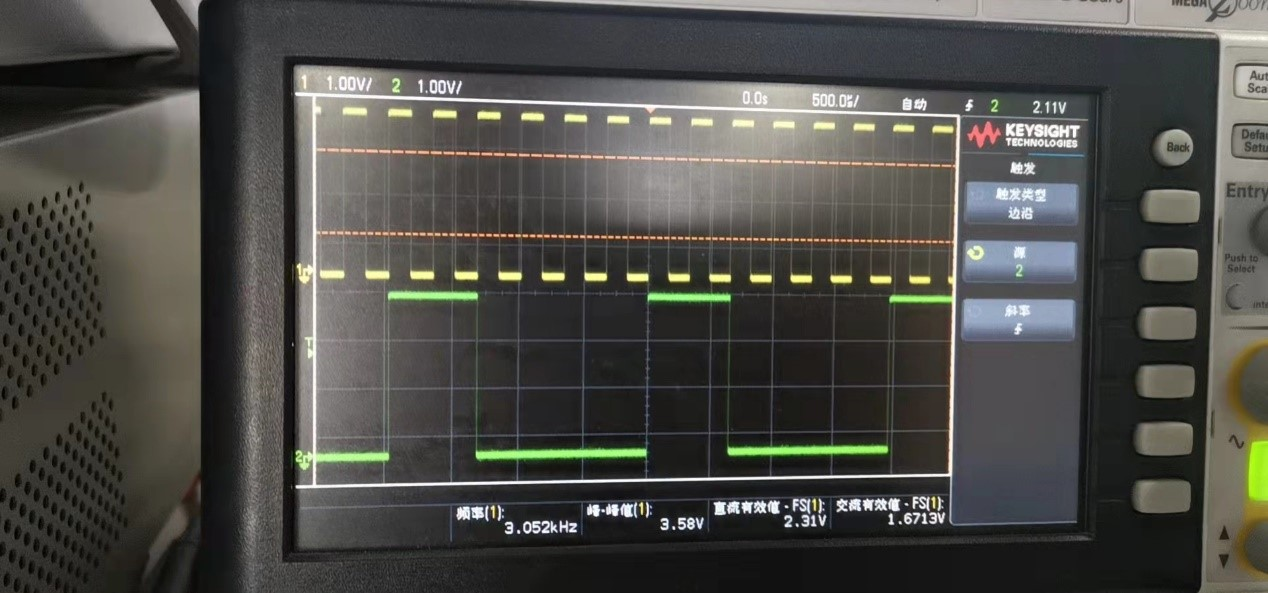
\includegraphics[width=0.45\textwidth]{6set9/jb2.jpg}}
    \subfigure[\(JB_3\)]{
    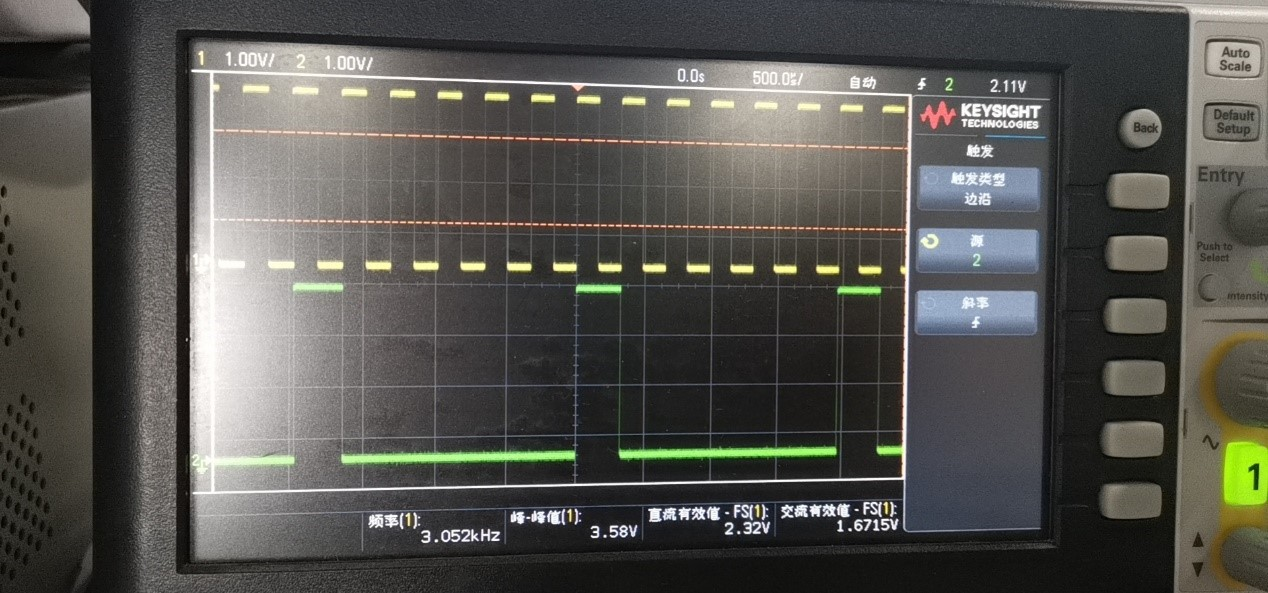
\includegraphics[width=0.45\textwidth]{6set9/jb3.jpg}}
    \subfigure[\(JB_4\)]{
    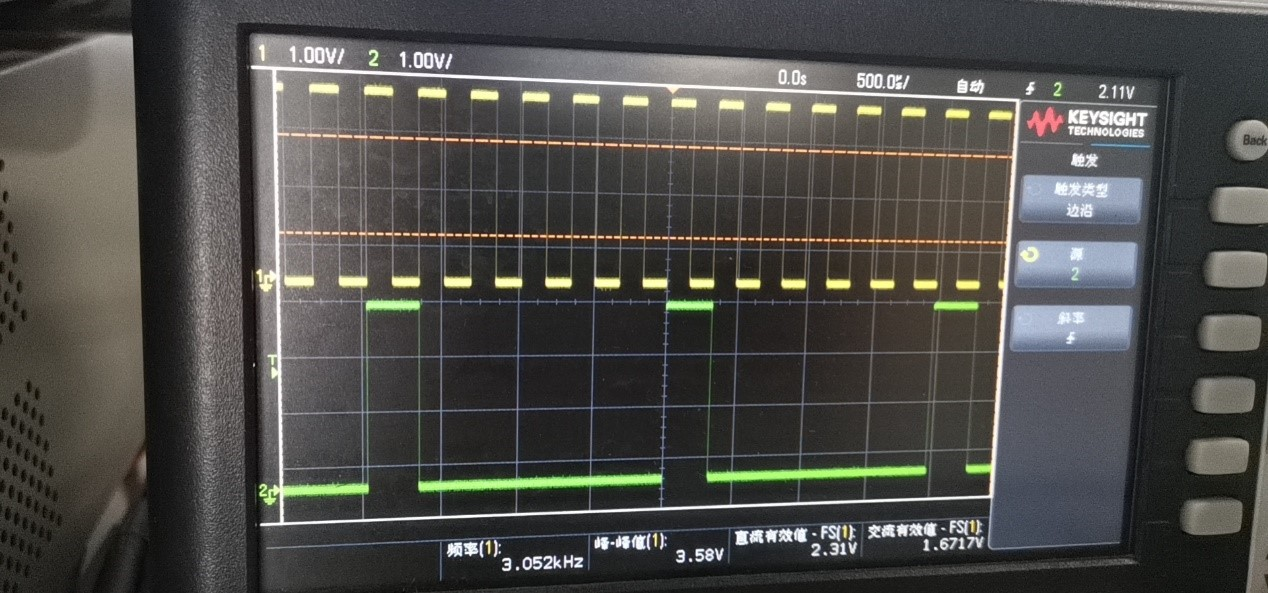
\includegraphics[width=0.45\textwidth]{6set9/jb4.jpg}}

    \caption{六进制计数器引脚输出波形}
    \label{6set9}
\end{figure}

\subsubsection{小结}
\begin{itemize}
    \item 熟悉了计数器置数端的用法,掌握了利用置数端以及置零端使计数器数字归零,调整进位的方法。
    \item 利用置9法,实现了六进制计数器。
\end{itemize}




\section{实验总结}


\section*{原始数据}
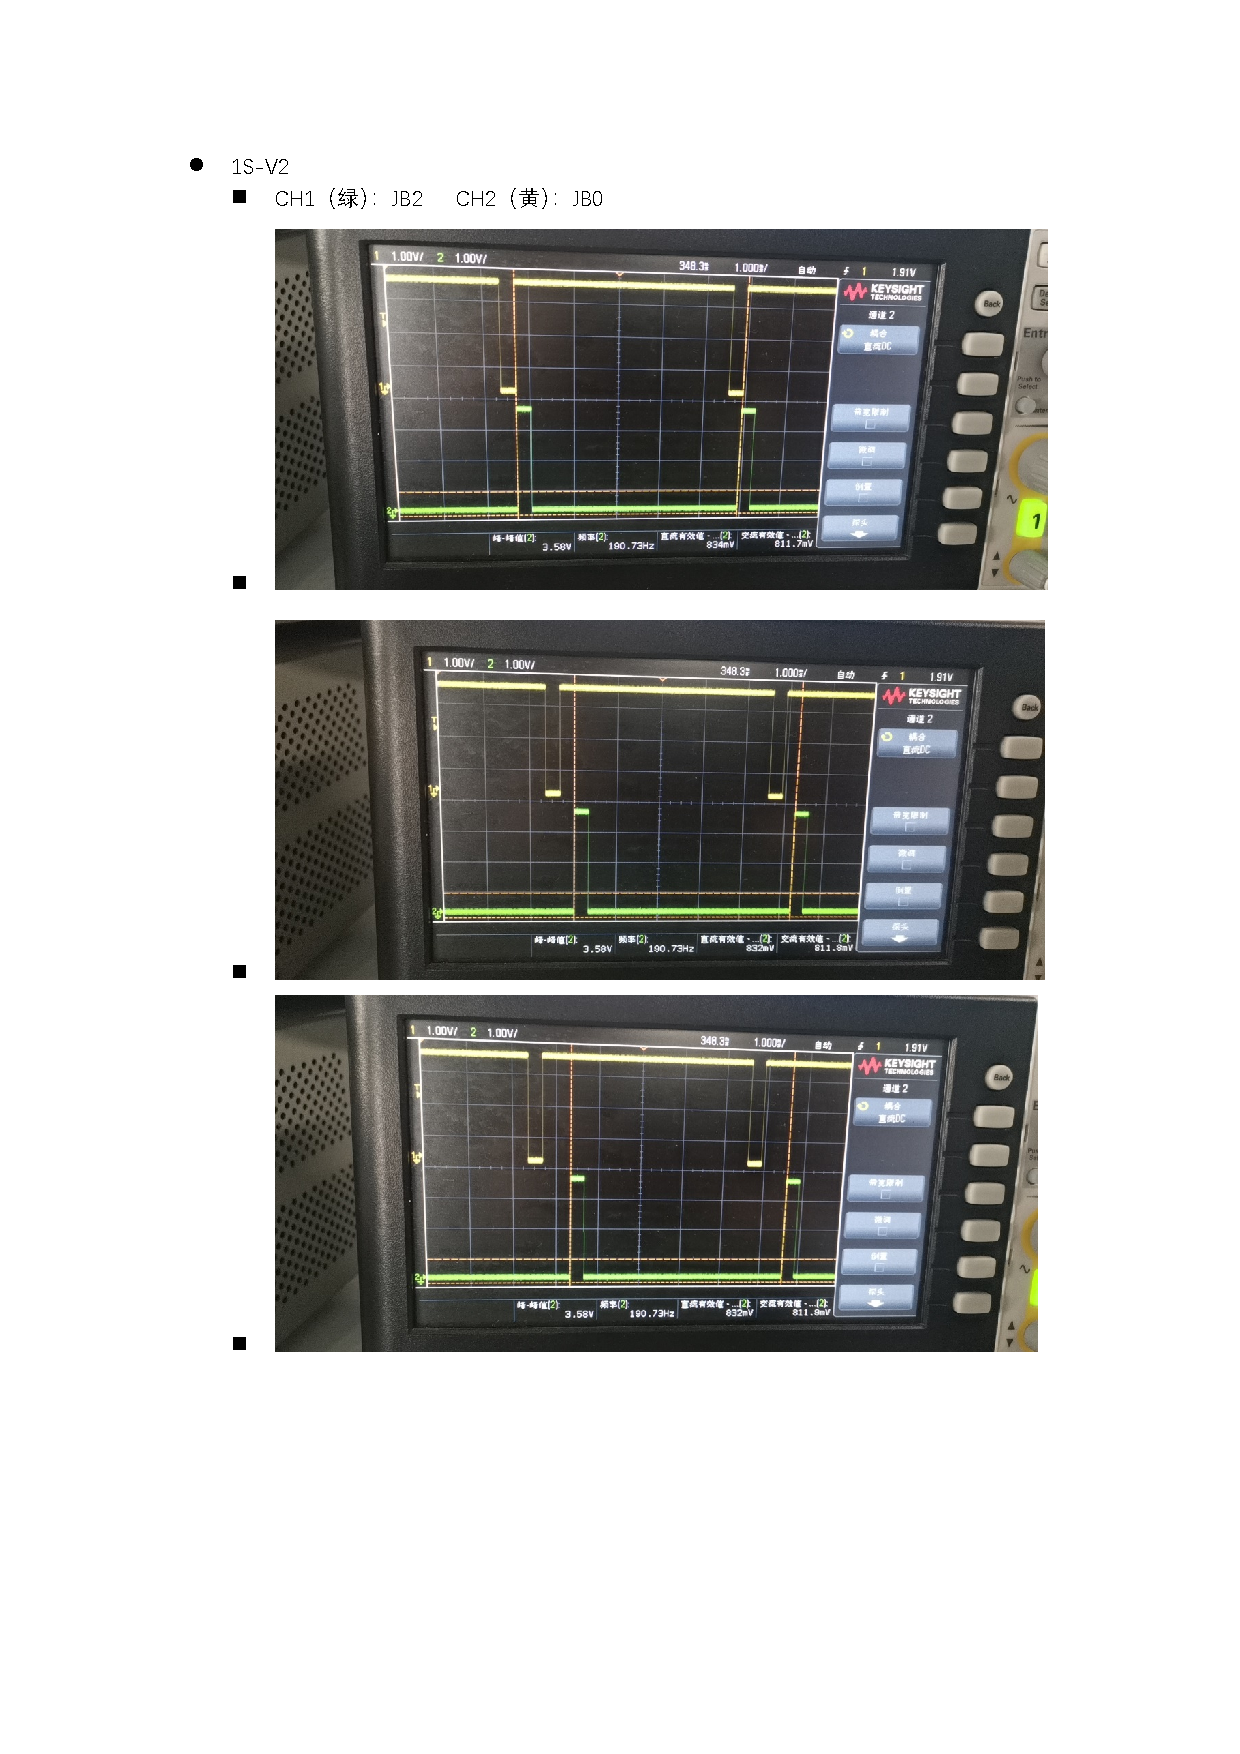
\includepdf[pages=1-7]{exp_data.pdf}

\end{document}